\documentclass[12pt]{book}

% ------------------------------------------------
% Packages for math and formatting
% ------------------------------------------------
\usepackage{amsmath, amssymb}
\usepackage{graphicx}
\usepackage{float}
\usepackage{caption}
\usepackage{subcaption}
\usepackage{tikz}
\usepackage{pgfplots}
\pgfplotsset{compat=1.18}
\usepackage{multicol}
\usepackage{enumitem}
\usepackage{tabularx}
\usepackage{lmodern}
\usepackage[authoryear]{natbib}

% ------------------------------------------------
% Typography and better fonts
% ------------------------------------------------
\usepackage{newtxmath} % or use mathpazo / newtxtext,newtxmath

\usepackage[a4paper, inner=1.2in, outer=1in, top=1in, bottom=1in]{geometry}

% Listings package for beautiful code formatting
\usepackage{listings}
\usepackage{xcolor} % for color customization

% Define custom C++ style
\lstdefinestyle{cppstyle}{
  language=C++,
  backgroundcolor=\color{gray!10},          % Soft gray background
  basicstyle=\ttfamily\footnotesize,        % Monospaced font, slightly smaller
  keywordstyle=\color{blue!70!black}\bfseries,  % Darker blue keywords
  commentstyle=\color{gray!70!black}\itshape,   % Dark gray italic comments
  stringstyle=\color{green!50!black},       % Strings in green
  numberstyle=\tiny\color{gray},            % Line numbers styling
  numbers=left,                             % Line numbers on the left
  numbersep=10pt,                           % Space between numbers and code
  tabsize=4,                                % Tab width
  showstringspaces=false,                   % Don't mark spaces in strings
  breaklines=true,                          % Break lines if too long
  breakatwhitespace=true,                   % Break only at whitespace
  frame=tb,                                 % Top and bottom borders
  captionpos=b,                             % Caption at the bottom
  escapeinside={(*@}{@*)},                  % For LaTeX inside code
  morekeywords={parallel, atomic, shared},  % Add any parallel-specific keywords here
}

% Use this style with:
% \begin{lstlisting}[style=cppstyle, caption={Your caption}, label={lst:yourlabel}]
% Your C++ code
% \end{lstlisting}



% ------------------------------------------------
% Boxed environments (Example, Note, Intuition)
% ------------------------------------------------
\usepackage{tcolorbox}
\tcbuselibrary{skins, breakable}

\newtcolorbox{example}{
  enhanced,
  breakable,
  colback=blue!5!white,
  colframe=blue!75!black,
  fonttitle=\bfseries,
  title=Example,
  sharp corners=south,
  boxrule=0.5pt,
  arc=4pt,
  left=6pt, right=6pt, top=6pt, bottom=6pt,
  before skip=10pt, after skip=10pt
}

\newtcolorbox{intuition}{
  enhanced,
  breakable,
  colback=yellow!10,
  colframe=orange!85!black,
  fonttitle=\bfseries,
  title=Intuition,
  sharp corners=south,
  boxrule=0.5pt,
  arc=4pt,
  left=6pt, right=6pt, top=6pt, bottom=6pt,
  before skip=10pt, after skip=10pt
}

\newenvironment{note}
{
    \begin{center}
    \begin{tikzpicture}
    \node[rectangle, draw=black!50, top color=black!10, bottom color=black!10, rounded corners=0.5cm, inner xsep=0.5cm, inner ysep=0.5cm] 
    \bgroup
    \begin{minipage}{0.9\textwidth}
}
{
    \end{minipage}
    \egroup;
    \end{tikzpicture}
    \end{center}
}

% ------------------------------------------------
% Hyperlinks and metadata
% ------------------------------------------------
\usepackage{hyperref}
\hypersetup{
    colorlinks=true,
    linkcolor=blue,
    filecolor=magenta,
    urlcolor=cyan,
    pdftitle={Notes on Parallel Computing},
    pdfauthor={Nihar Shah},
    pdfkeywords={Parallel Computing, OpenMP, MPI, CUDA, HPC},
}

\newcommand{\weblink}[2]{\href{#1}{\textcolor{blue}{#2}}}

% ------------------------------------------------
% Headers and footers
% ------------------------------------------------
\usepackage{fancyhdr}
\usepackage{lastpage}
\setlength{\headheight}{14.49998pt}
\pagestyle{fancy}
\fancyhf{}
\rhead{Page \thepage\ of \pageref{LastPage}}
\lhead{Parallel Computing}
\renewcommand{\headrulewidth}{1pt}
\renewcommand{\footrulewidth}{1pt}

% ------------------------------------------------
% Chapter and TOC styling (Optional)
% ------------------------------------------------
\usepackage{titlesec}
\titleformat{\chapter}[display]
  {\normalfont\bfseries\Huge}{\chaptername\ \thechapter}{20pt}{\Huge}

\usepackage{tocloft}
\renewcommand{\cftchapfont}{\bfseries}
\renewcommand{\cftchappagefont}{\bfseries}

% Optional: chapters start without blank page
\let\cleardoublepage\clearpage

% ------------------------------------------------
% Start document
% ------------------------------------------------
\begin{document}

\frontmatter
\title{Notes on Parallel Computing}
\author{Nihar Shah}
\date{\today}
\maketitle

\tableofcontents
\mainmatter

\chapter{Computer Architecture} \label{chap:computer-architecture}

\begin{note}
    Here, it is assumed that the reader has a basic beginner-level understanding of the C programming language.
\end{note}
For a gentler introduction refer to first four YouTube lectures by Prof. Mathew Jacob on High Performance Computing (HPC)~\cite{nptel-hpc-intro}.

\section{How is Data Represented?} \label{sec:data-represented}

In a digital computer, data is represented in binary form. This means everything—from numbers to text—is stored using only two symbols: 0 and 1.

The smallest unit of data is called a \textbf{bit}. A bit can take only two values: 0 or 1.

Some commonly used units of data are:
\begin{itemize}
    \item \textbf{bit (b)} — smallest unit of data
    \item \textbf{Byte (B)} — 1 Byte = 8 bits
    \item \textbf{Kilobyte (KB)} — $1\ \text{KB} = 2^{10}$ Bytes = 1024 Bytes
    \item \textbf{Megabyte (MB)} — $1\ \text{MB} = 2^{20}$ Bytes
    \item \textbf{Gigabyte (GB)} — $1\ \text{GB} = 2^{30}$ Bytes
\end{itemize}

These units are based on powers of two because binary is the foundation of all digital computation.

\medskip

For example, character data is often represented using an 8-bit code. In many systems, a 7-bit code is used to encode the character itself, and 1 extra bit is added as a \textbf{parity bit}.

The purpose of the parity bit is to help check whether the character data is correct or not. It acts as a basic form of error detection—if a bit gets flipped accidentally during storage or transmission, the system can sometimes catch the mistake using this bit.

\subsection{Integer Data Representation} \label{subsec:integer-data}

Integer data can be of two types:
\begin{itemize}
    \item \textbf{Signed Integer} — This type of integer can represent both positive and negative values. The most significant bit (MSB) is used to indicate the sign of the number:
    \begin{itemize}
        \item $0$ for positive numbers
        \item $1$ for negative numbers
    \end{itemize}
    
    Suppose $x_{n-1}x_{n-2}\ldots x_0$ is an $n$-bit signed integer. Then its value can be calculated using:
    \begin{equation} \label{eq:signed-magnitude}
        x_{n-1}x_{n-2}\ldots x_0 = (-1)^{x_{n-1}} + \sum_{i=0}^{n-2} x_i 2^i
    \end{equation}
    Here, $x_0$ is the least significant bit (LSB) and $x_{n-1}$ is the most significant bit (MSB), which represents the sign.

    \medskip
    \textbf{Two's Complement}\\
    Another way to represent signed integers is using \textbf{Two's Complement}. In this method, negative numbers are represented by inverting all bits of their positive counterpart and then adding 1 to the result.

    The value of a signed integer in two's complement form is computed as:
    \begin{equation} \label{eq:twos-complement}
        x_{n-1}x_{n-2}\ldots x_0 = -x_{n-1} \cdot 2^{n-1} + \sum_{i=0}^{n-2} x_i 2^i
    \end{equation}
    This representation allows the same hardware to perform both signed and unsigned arithmetic, which makes it widely used.

    \begin{example}
        \textbf{Steps to convert a negative decimal number to its two's complement representation:}
        \begin{enumerate}
            \item Convert the absolute value of the number to binary.
            \item Add a 0 (or 0s) in front if needed to reach the desired number of bits.
            \item Flip all 0s to 1s and 1s to 0s.
            \item Add 1 to the result.
        \end{enumerate}

        Let's take $-14$ as an example.

        \begin{itemize}
            \item The binary of $14$ is $1110$.
            \item To convert this to 5-bit representation, we pad a 0 in front: $01110$.
            \item Now, flip the bits: $10001$.
            \item Add 1: $10001 + 1 = 10010$.
        \end{itemize}

        So, the two's complement representation of $-14$ in 5 bits is $10010$.

        \medskip
        Similarly, to represent $-14$ in 32 bits:
        \begin{itemize}
            \item Binary of $14$: $1110$.
            \item Pad with zeros: $000\ldots0001110$ (total 32 bits).
            \item Flip all bits: $111\ldots1110001$.
            \item Add 1: $111\ldots1110010$.
        \end{itemize}

        Thus, $111\ldots1110010$ is the two's complement representation of $-14$ in 32 bits.
        Thus, the decimal number $-14_{10}$ using two's complement:
        \begin{itemize}
            \item In 5 bits: $10010$ (i.e., $-16 + 2$)
            \item In 6 bits: $110010$ (i.e., $-32 + 16 + 2$)
            \item In 32 bits: $111\ldots1110010$
        \end{itemize}
    \end{example}

    \begin{note}
    Note that in Two's complement representation, positive numbers are represented identically to their standard binary form. For example, to represent the number $65$ as a $32$-bit signed integer using Two's complement, we simply write its binary form padded with leading zeros:

    \[
    65 = 00000000\ 00000000\ 00000010\ 00000001
    \]

    Here, the most significant bit (MSB) is $0$, indicating a non-negative number. Since $65$ is positive, no bit inversion or addition is needed — the representation remains the same as the unsigned binary version.
\end{note}


    \item \textbf{Unsigned Integer} — This type of integer can only represent non-negative values. It does not use any sign bit, so all bits contribute to the magnitude of the number.

    If $x_{n-1}x_{n-2}\ldots x_0$ is an $n$-bit unsigned integer, then its value is computed using:
    \begin{equation} \label{eq:unsigned}
        x_{n-1}x_{n-2}\ldots x_0 = \sum_{i=0}^{n-1} x_i 2^i
    \end{equation}

\item \textbf{Hexadecimal} — This is a base-16 number system. It uses the following 16 symbols to represent values: \texttt{0, 1, 2, 3, 4, 5, 6, 7, 8, 9, A, B, C, D, E, F}.

Each hexadecimal digit corresponds to a unique 4-bit binary sequence. That is why we need at least 4 bits to represent a single hexadecimal digit. For example:
\[
A_{16} = 1010_2
\]

Let us take another example. The decimal number $14$ in 32-bit binary representation is:
\[
0000\ldots00001110
\]
In two's complement form (to represent $-14$), it becomes:
\[
1111\ldots11110010
\]
This binary sequence corresponds to the hexadecimal value \texttt{FFFFFFF2}. In C programming, we often prefix hexadecimal constants with \texttt{0x}, so this would be written as \texttt{0xFFFFFFF2}.

\medskip
The table below shows how each hexadecimal digit maps to its binary equivalent:

\begin{center}
\begin{tabular}{|c|c|}
\hline
\textbf{Hexadecimal} & \textbf{Binary} \\
\hline
0 & 0000 \\
1 & 0001 \\
2 & 0010 \\
3 & 0011 \\
4 & 0100 \\
5 & 0101 \\
6 & 0110 \\
7 & 0111 \\
8 & 1000 \\
9 & 1001 \\
A & 1010 \\
B & 1011 \\
C & 1100 \\
D & 1101 \\
E & 1110 \\
F & 1111 \\
\hline
\end{tabular}
\end{center}

\item \textbf{Real Data} — Real numbers are usually represented using floating point notation. This means the decimal point can ``float" to any position, allowing us to represent both very small and very large numbers efficiently.

In contrast, \textbf{fixed point} representation reserves a fixed number of bits for the integer and fractional parts, and the decimal point is fixed in one place. For example, suppose we allocate (1 bit for sign, 8 bits for integer part and 7 bits for fractional part):

\[
\underbrace{0}_{\text{sign bit}} \underbrace{00001101}_{\text{integer part}} \cdot \underbrace{0110000}_{\text{fractional part}}
\]
This represents $13.25$ because $00001101_2 = 13$ and $0110000_2 = 0.25$.

\medskip
\textbf{IEEE 754 Floating Point Standard:} Real numbers in modern computers are represented using the IEEE 754 standard. For a 32-bit float, the layout is as follows:
\begin{itemize}
    \item \textbf{Sign Bit (1 bit):} It is the most significant bit. It is $0$ for positive numbers and $1$ for negative numbers.
    \item \textbf{Exponent (8 bits):} These next 8 bits store the exponent. The value stored here is in \textit{Excess-127} or \textit{Bias-127} format, which means the actual exponent is: 
    \[
    \text{Exponent}_{\text{actual}} = \text{Exponent}_{\text{stored}} - 127
    \]
    \item \textbf{Fraction (23 bits):} These represent the fractional part of the number. The full number is stored in normalized form as $1.f$, where $f$ is the binary fractional part.
\end{itemize}

The floating point number represented is:
\[
(-1)^s \times 1.f \times 2^{e - 127}
\]

\medskip
\textbf{Steps to convert a real number to IEEE 754 format:}
\begin{enumerate}
    \item Convert the number to binary.
    \item Normalize it to the form $1.f \times 2^e$.
    \item Add $127$ to the exponent value.
    \item Determine the sign bit ($0$ for positive, $1$ for negative).
    \item Write the exponent in 8-bit binary.
    \item Write the fraction after the decimal point in 23-bit binary.
\end{enumerate}

\begin{example}
Let’s convert $-23.5_{10}$ to IEEE 754 format:

\begin{itemize}
    \item Binary: $-10111.1_2$
    \item Normalized: $-1.01111 \times 2^4$
    \item Exponent: $4 + 127 = 131_{10} = 10000011_2$
    \item Fraction: $01111000000000000000000$ (pad 0s to make 23 bits)
    \item Sign bit: $1$
\end{itemize}

So the 32-bit IEEE 754 representation is:
\[
\boxed{1~10000011~01111000000000000000000}
\]
and is \texttt{0xC1BC0000} in hexadecimal.
\end{example}

\medskip
\textbf{Steps to convert IEEE 754 to decimal:}
\begin{enumerate}
    \item Interpret the sign bit.
    \item Convert the exponent bits to decimal and subtract 127.
    \item Convert the fraction to decimal by treating it as $1.f$.
    \item Multiply the result by $(-1)^s$ and $2^{e - 127}$.
\end{enumerate}

\begin{example}
Let us convert the IEEE 754 number:
\[
1~10000001~01100000000000000000000
\]
\begin{itemize}
    \item Sign bit: $1$ (so the number is negative)
    \item Exponent: $129$ $\Rightarrow$ $129 - 127 = 2$
    \item Fraction: $1.011$
\end{itemize}
So the final number is:
\[
-1 \times 1.011 \times 2^2 = -101.1_2 = -5.5_{10}
\]
\end{example}

\medskip
\textbf{Advantages and Limitations:} Floating point allows us to represent a very large range of values. It avoids the limitation of fixed decimal positions. However, it can suffer from rounding errors and loss of precision over many operations.

\medskip
\textbf{Special Cases (B\&O 2.4.2):}
\begin{itemize}
    \item \textbf{Zero:} All exponent and fraction bits are 0.
    \begin{itemize}
        \item $+0$: Sign bit $0$
        \item $-0$: Sign bit $1$
    \end{itemize}
    \item \textbf{Infinity:} Exponent bits are all $1$, fraction bits are all $0$.
    \begin{itemize}
        \item $+\infty$: Sign bit $0$
        \item $-\infty$: Sign bit $1$
    \end{itemize}
\end{itemize}
Such special cases are summarised in the following tables~\ref{tab:ieee754-special} and ~\ref{tab:ieee754-operations}. For more details on this topics refer~\cite{rajaraman2016ieee}.
\begin{table}[H]
\centering
\renewcommand{\arraystretch}{1.4}
\begin{tabularx}{\textwidth}{|X|c|c|X|}
\hline
\textbf{Value} & \textbf{Sign} & \textbf{Exponent (8 bits)} & \textbf{Significand (23 bits)} \\
\hline
$+0$ & 0 & 00000000 & 00…00 (all 23 bits 0) \\
\hline
$-0$ & 1 & 00000000 & 00…00 (all 23 bits 0) \\
\hline
$+1.f \times 2^{(e-b)}$ & 0 & 00000001 to 11111110 & $a\,a\,\ldots\,a$ (where $a=0$ or $1$) \\
\hline
$-1.f \times 2^{(e-b)}$ & 1 & 00000001 to 11111110 & $a\,a\,\ldots\,a$ (where $a=0$ or $1$) \\
\hline
$+\infty$ & 0 & 11111111 & 00…00 (all 23 bits 0) \\
\hline
$-\infty$ & 1 & 11111111 & 00…00 (all 23 bits 0) \\
\hline
SNaN (Signaling NaN) & 0 or 1 & 11111111 & 000…01 to 011…11 (leading bit 0, at least one 1) \\
\hline
QNaN (Quiet NaN) & 0 or 1 & 11111111 & 1000…10 (leading bit 1) \\
\hline
Positive subnormal $0.f \times 2^{x+1-b}$ & 0 & 00000000 & 000…01 to 111…11 (at least one 1) \\
\hline
\end{tabularx}
\caption{IEEE 754 Representation for Special Floating-Point Values (32-bit)}
\label{tab:ieee754-special}
\end{table}

\begin{table}[H]
\centering
\renewcommand{\arraystretch}{1.4}
\begin{tabularx}{\textwidth}{|>{\centering\arraybackslash}X|>{\centering\arraybackslash}X|
                                >{\centering\arraybackslash}X|>{\centering\arraybackslash}X|}
\hline
\textbf{Operation} & \textbf{Result} \\
\hline
$n / \pm \infty$ & $0$ \\
\hline
$\pm 0 / \pm 0$ & NaN\\
\hline
$\pm \infty / \pm \infty$ & $\pm \infty$ \\
\hline
$\infty - \infty$ & NaN\\
\hline
$\pm n / 0$ & $\pm \infty$ \\
\hline
$\pm \infty / \pm \infty$ & NaN\\
\hline
$\infty + \infty$ & $\infty$ \\
\hline
$\pm \infty \times 0$ & NaN \\
\hline
\end{tabularx}
\caption{Results of Floating Point Operations Involving Infinity and Zero}
\label{tab:ieee754-operations}
\end{table}

\begin{note}
    Note that table~\ref{tab:ieee754-special} can be similarly extended for 64-bit representations. Here's a fun question to think about: What is the largest number that can be represented in 32-bit IEEE 754 format (excluding special values like $+\infty$)?

    A natural answer might be: all $1$s in the exponent bits and all $1$s in the significand (fraction) bits. However, this combination represents a NaN (Not a Number), since according to the IEEE 754 standard, an exponent of all $1$s and a non-zero significand encodes a NaN.

    Therefore, the largest representable finite number in 32-bit IEEE 754 format corresponds to an exponent of $11111110$ (i.e., $254$ in decimal), and a significand of all $1$s (i.e., the largest fraction just below 1). This gives the largest normal floating-point number just before $+\infty$.

    Similarly, for the smallest positive number (magnitude-wise) in 64-bit representation, it is not simply all zeros, since that would correspond to $+0$ (or $-0$ if the sign bit is $1$). There are two interpretations of the “smallest number”:
    \begin{itemize}
        \item The smallest \textbf{positive} subnormal number is represented by: sign bit = $0$, exponent = all $0$s, and fraction = $000\ldots 01$. This is the smallest positive number greater than zero.
        \item The smallest \textbf{(most negative) representable number} is given by: sign bit = $1$, exponent = $111\ldots10$, and fraction = all $1$s. This is the largest-magnitude negative number (i.e., most negative finite number).
    \end{itemize}
\end{note}


\medskip
\textbf{Handling Overflow in Arithmetic:}

Sometimes, the result of a floating point operation might not fit in the 23-bit significand. In such cases, we have two options:
\begin{itemize}
    \item \textbf{Truncation:} Discard extra bits.
    \item \textbf{Rounding:}
    \begin{itemize}
        \item Rounding upwards: For example, if significand is $0.110\ldots 01$ and overflow is by $1$, then the significand after rounding becomes $0.110\ldots 10$, i.e. we add $1$ to the LSB.
        \item Rounding downwards: The extra bits are ignored.
    \end{itemize}
\end{itemize}

\medskip
\subsection*{IEEE 754 for 64-bit (Double Precision):}  
For higher precision, we use 64-bit representation:
\begin{itemize}
    \item $1$ bit for sign
    \item $11$ bits for exponent
    \item $52$ bits for fraction
\end{itemize}
\end{itemize}

\subsection{Variables and Data Allocation of Different Lifetimes}

Understanding these memory regions and their respective allocation strategies is fundamental to writing safe and efficient programs, particularly in low-level languages like C and C++. Mistakes such as forgetting to free heap memory, or accessing memory after it has been deallocated, are common sources of bugs and security vulnerabilities. 
In a computer program, different variables have different lifetimes, depending on where and how they are declared and allocated. These lifetimes determine how long a variable remains in memory during the program's execution. Broadly, there are three primary types of data allocation:

\begin{itemize}
    \item \textbf{Static Allocation:} 
    Variables that are statically allocated exist for the entire duration of the program. Their lifetime spans from the beginning to the end of program execution. This includes global variables, as well as static local variables declared with the \texttt{static} keyword in C. These variables are allocated in the data segment of the memory, which is part of the executable file. Since their memory is reserved at compile-time, the size and type of statically allocated data must be known in advance. Both initialized and uninitialized static variables are handled this way: 
    \begin{itemize}
        \item Initialized static data is stored in the `.data` segment.
        \item Uninitialized static data (commonly zero-initialized) is stored in the `.bss` segment.
    \end{itemize}

    \item \textbf{Heap Allocation:}
    Heap allocation is used for dynamically allocated data, whose size may not be known at compile-time. This type of allocation allows a program to request and release memory at runtime using functions such as \texttt{malloc}, \texttt{calloc}, or \texttt{realloc} in C. The memory must be explicitly freed using \texttt{free} when it is no longer needed, to avoid memory leaks. The lifetime of a heap-allocated variable begins when it is allocated and ends when it is explicitly deallocated. All such allocations happen in the memory region known as the heap. This is particularly useful when dealing with:
    \begin{itemize}
        \item Variable-sized data structures (e.g., linked lists, trees, graphs)
        \item Data that must persist across function calls
    \end{itemize}

    \item \textbf{Stack Allocation:}
    Stack allocation is used for variables that are declared inside functions, including function parameters and local variables. These variables are allocated on the call stack, a special region of memory used to manage function calls and returns. The lifetime of a stack-allocated variable is confined to the duration of the function in which it is declared. That is, memory for such variables is allocated when the function is invoked and deallocated when the function returns. This makes stack allocation highly efficient, as it simply involves moving the stack pointer up and down. However, stack variables are not accessible once the function ends, and returning pointers to such variables leads to undefined behavior.
\end{itemize}
For example, when a program begins execution, its memory is organized into distinct regions, as shown in Figure~\ref{fig:memory_layout}.

\begin{figure}[h!]
    \centering
    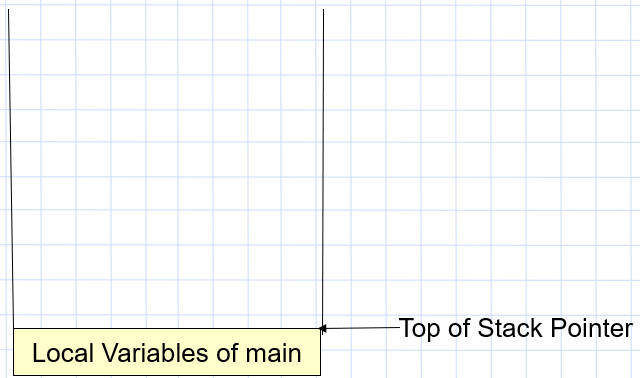
\includegraphics[width=0.8\textwidth]{images/memory_layout.png}
    \caption{Memory Layout of a Program}
    \label{fig:memory_layout}
\end{figure}

The stack pointer initially points to the top of the stack, which holds the local variables of the \texttt{main()} function. The stack grows downward (towards lower memory addresses), and this region of memory is used to manage function calls and their associated data.

Now suppose the \texttt{main()} function makes a call to another function, say \texttt{func1()}. In that case, the system allocates additional space on the stack for the function call. This includes space for:
\begin{itemize}
    \item The return address (i.e., the point in \texttt{main()} to resume execution after \texttt{func1()} finishes),
    \item Any arguments passed to \texttt{func1()},
    \item The local variables declared inside \texttt{func1()}.
\end{itemize}

This updated stack state is illustrated in Figure~\ref{fig:memory_layout_func1}. The stack pointer is now moved to point to the new top of the stack, corresponding to the local variables of \texttt{func1()}.

\begin{figure}[h!]
    \centering
    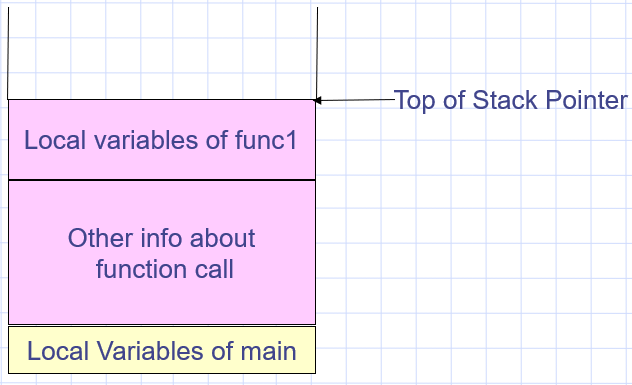
\includegraphics[width=0.8\textwidth]{images/memory_layout_func1.png}
    \caption{Memory Layout after a Function Call to \texttt{func1()}}
    \label{fig:memory_layout_func1}
\end{figure}

When \texttt{func1()} completes its execution and returns, the stack frame associated with it is deallocated. This involves:
\begin{itemize}
    \item Removing the local variables of \texttt{func1()},
    \item Restoring the return address,
    \item Adjusting the stack pointer back to its state before the call.
\end{itemize}

As a result, the stack pointer once again points to the top of the stack containing the local variables of \texttt{main()}, restoring the memory layout to its original state shown in Figure~\ref{fig:memory_layout}.
This mechanism of pushing function call data onto the stack and popping it off during function return is fundamental to how most programming languages, including C, manage nested and recursive function calls. It also underpins the concept of function call stacks and stack-based memory management.

\subsection{Program and Data}

When a program is compiled and executed, its memory layout is broadly divided into several segments, each serving a specific purpose. These include the code segment, data segments (initialized and uninitialized), heap, and stack.

The code is stored in the \textbf{text segment}, which contains the compiled machine instructions of the program. This segment is typically read-only and does not change during execution.

The \textbf{data segment} holds global and static variables. It is further divided into:
\begin{itemize}
    \item \textbf{Initialized Data Segment:} Contains global and static variables that are initialized by the programmer.
    \item \textbf{Uninitialized Data Segment (also called BSS):} Contains global and static variables that are declared but not explicitly initialized.
\end{itemize}
Both the code and data segments are fixed in size once the program starts running.

In contrast, two other regions of memory — the \textbf{heap} and the \textbf{stack} — are dynamic in nature:
\begin{itemize}
    \item The \textbf{heap} is used for dynamically allocated memory (e.g., using \texttt{malloc()} in C). The heap grows upwards as new memory is allocated during program execution.
    \item The \textbf{stack} is used for function call information, such as local variables, parameters, and return addresses. It grows downwards and shrinks as functions are called and returned.
\end{itemize}

This division and organization of memory during program execution is beautifully depicted in Figure~\ref{fig:program_data}.

\begin{figure}[H]
    \centering
    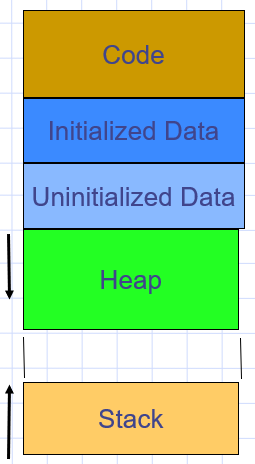
\includegraphics[width=0.25\textwidth]{images/program_data.png}
    \caption{Program and Data Memory Layout}
    \label{fig:program_data}
\end{figure}
A program utilizes the main memory in a structured way, with different sections allocated for different types of data and instructions. 

For instance, an instruction such as \texttt{add x, y, z} would be stored in the \textbf{text segment} (also referred to as the code segment) of the memory. This segment contains the compiled machine instructions that the CPU executes. It is typically read-only to prevent accidental overwriting of program instructions during execution.

The variables used in a program, on the other hand, are allocated in different memory segments depending on their lifetime and declaration style:

\begin{itemize}
    \item An integer variable like \texttt{int x}, if declared within a function, is likely to be \textbf{stack-allocated}. This means that memory for \texttt{x} is reserved on the call stack, and its lifetime is limited to the duration of the function's execution.
    
    \item A variable like \texttt{double w}, if allocated dynamically using functions such as \texttt{malloc()} or \texttt{calloc()}, is stored in the \textbf{heap segment}. The programmer must manage the lifetime of such variables explicitly using memory allocation and deallocation functions.
    
    \item A variable such as \texttt{float t}, if declared globally or as a static local variable, is stored in the \textbf{data segment}. This data segment can be further divided into:
    \begin{itemize}
        \item The \textbf{initialized data segment}, where variables with an explicit initial value reside.
        \item The \textbf{uninitialized data segment} (often called the BSS segment), which holds variables declared but not explicitly initialized.
    \end{itemize}
\end{itemize}

This organization of memory usage is depicted in Figure~\ref{fig:program_memory}.

\begin{figure}[H]
    \centering
    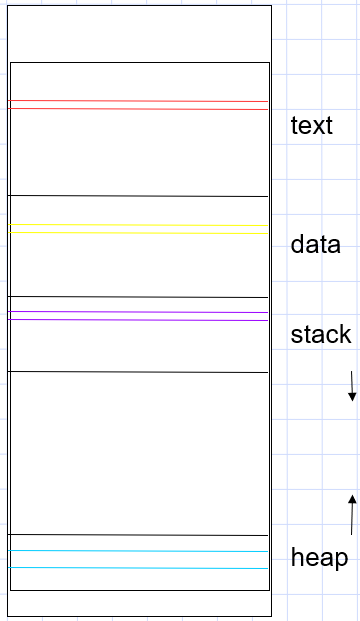
\includegraphics[width=0.5\textwidth]{images/program_memory.png}
    \caption{Program Memory Layout}
    \label{fig:program_memory}
\end{figure}


\section{Basic Computer Organization}

A computer system is broadly organized into three major components, as illustrated in Figure~\ref{fig:computer_organization}:

\begin{itemize}
    \item \textbf{Central Processing Unit (CPU) or Processor:} Often referred to as the brain of the computer, the CPU is responsible for executing instructions and performing all arithmetic and logical operations.
    
    \item \textbf{Main Memory:} This component is used to store both data and instructions temporarily during program execution. Memory is essential for the CPU to retrieve and process data efficiently.
    
    \item \textbf{Input/Output Devices (I/O Devices):} These devices enable the computer to interact with the external environment. Examples include keyboards, mice, monitors, and printers. Input devices send data to the computer, while output devices display or produce results.
\end{itemize}

\begin{figure}[H]
    \centering
    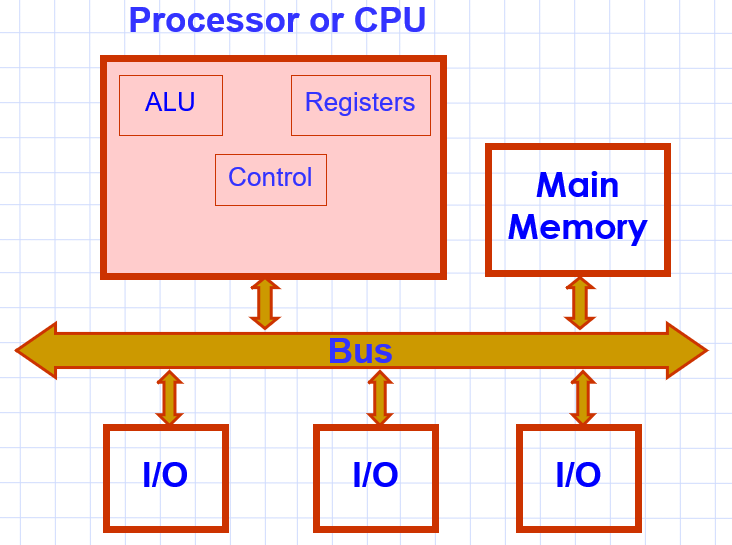
\includegraphics[width=0.5\textwidth]{images/computer_organization.png}
    \caption{Basic Computer Organization}
    \label{fig:computer_organization}
\end{figure}

The CPU itself is further divided into the following core components:

\begin{itemize}
    \item \textbf{Control Unit (CU):} The control unit manages and coordinates the operations of the CPU. It directs how data moves between the CPU, memory, and I/O devices. It decodes instructions and ensures that the correct sequence of operations is followed.

    \item \textbf{Arithmetic Logic Unit (ALU):} This unit performs all arithmetic operations (like addition, subtraction) and logical operations (like AND, OR, NOT). It acts as the computational engine of the CPU.

    \item \textbf{Registers:} Registers are small, high-speed storage locations built directly into the CPU. They hold temporary data and intermediate results while instructions are being executed. Registers play a key role in speeding up the processing as accessing them is significantly faster than accessing main memory.
    
    Registers are generally classified into two categories:
    \begin{itemize}
        \item \textbf{General Purpose Registers (GPRs):} These registers are available to the programmer for storing temporary values, such as operands or intermediate results. They help in reducing memory accesses. However, CPUs typically have a limited number of GPRs. One reason for using them is that there exists a large speed disparity between the CPU and main memory. For example:
        \begin{itemize}
            \item CPU operates at around 2 GHz, which corresponds to about 0.5 nanoseconds per cycle.
            \item Main memory accesses typically take 50--100 nanoseconds.
        \end{itemize}
        Because of this gap, using registers instead of repeatedly accessing memory helps improve performance.

        \item \textbf{Special Purpose Registers (SPRs):} These are reserved for specific control functions within the CPU. An important example is the \textbf{Program Counter (PC)}, which holds the address of the next instruction to be executed. Other SPRs may include status registers, instruction registers, and stack pointers depending on the architecture.
    \end{itemize}
\end{itemize}

\subsection{Main Memory and its problems}

One of the primary performance bottlenecks in modern computer systems arises due to the significant speed gap between the CPU and the main memory. While CPUs operate at very high frequencies (in the order of gigahertz), main memory (typically DRAM) is much slower—approximately $100\times$ slower. As a result, even though the CPU is capable of executing instructions rapidly, it often ends up idling while waiting for data to be fetched from the main memory.

Another related limitation is the scarcity of CPU registers. These registers are extremely fast and are used to store immediate data required for computations. However, their number is very limited, which means most data must be retrieved from main memory, further aggravating the memory bottleneck.

\begin{example}
    Let's consider a toy example to understand the main memory organization where the main memory has a size of 128 Bytes, and it is divided into blocks of size 4 Bytes. Since the memory is byte-addressable, each of the 128 Bytes has a unique memory address. To uniquely represent each of these 128 addresses, we require:
    \[
    \log_2 128 = 7 \text{ bits}
    \]
    Hence, memory addresses will range from $0000000_2$ to $1111111_2$. 

    The total number of memory blocks is:
    \[
    \frac{128}{4} = 32 \text{ blocks}
    \]
    
    Thus the number of bits that are used to identify the block number (since there are 32 blocks):
    \[
    \log_2 32 = 5 \text{ bits}
    \]

    Each block contains 4 Bytes, which requires 2 bits to specify the offset within the block:
    \[
    \log_2 4 = 2 \text{ bits}
    \]
    
    Therefore, any 7-bit memory address can be broken down into:
    \[
    \underbrace{b_6b_5b_4b_3b_2}_{\text{Block address (5 bits)}} \underbrace{b_1b_0}_{\text{Offset (2 bits)}}
    \]
    \begin{itemize}
        \item \textbf{Block address (5 bits):} Specifies which of the 32 blocks contains the address.
        \item \textbf{Offset (2 bits):} Specifies which byte within the block is being addressed.
    \end{itemize}

    This layout allows the system to efficiently locate a specific byte in memory by first identifying the block and then using the offset to access the byte within that block as shown in figure~\ref{fig:memory_addressing}.
    \begin{figure}[H]
        \centering
        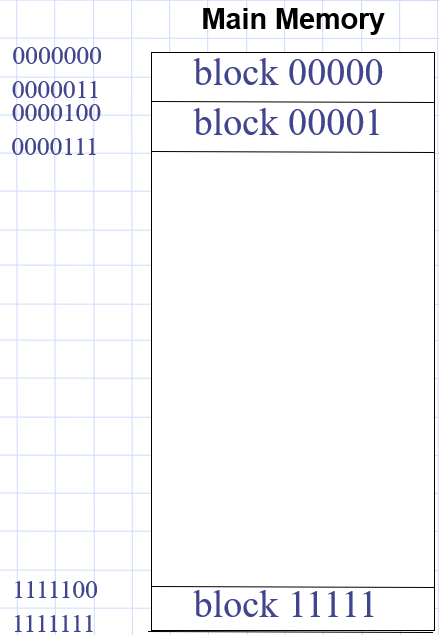
\includegraphics[width=0.5\textwidth]{images/memory_addressing.png}
        \caption{Memory Address Breakdown}
        \label{fig:memory_addressing}
    \end{figure}
\end{example}

\subsection{Cache Memory and Locality of Reference}
\textbf{The solution to this problem is the introduction of cache memory.} Cache is a small, high-speed memory that resides very close to or within the CPU itself. It acts as a buffer between the CPU and the main memory, storing frequently accessed data and instructions. If the data the CPU needs is found in the cache (called a \textit{cache hit}), it can be accessed much more quickly than from main memory. Otherwise, a \textit{cache miss} results in fetching data from the slower main memory.

The design of cache memory relies heavily on the \textbf{principle of locality of reference}, which exploits patterns in how programs access memory. There are two major types of locality:

\begin{itemize}
    \item \textbf{Temporal Locality:} This principle states that memory locations that have been accessed recently are least likely to be accessed again in the near future. For example, if a program accesses a variable, it is likely to access the same variable again soon. This is often seen in loops or repeated function calls where the same data is used multiple times.
    
    \item \textbf{Spatial Locality:} This principle states that memory locations near those that have been recently accessed are likely to be accessed soon. For instance, when iterating over an array, accessing one element implies that its neighboring elements will be accessed shortly.
\end{itemize}

By leveraging these two types of locality, cache memory significantly reduces the average memory access time and helps ensure that the CPU is not left waiting idly for data.


\section{Cache Composition}

Main memory is much larger than the cache. Hence, it is not possible to keep the entire memory content in the cache at once. So, when the CPU accesses a memory location, a portion of the memory which is a \textbf{memory block} is temporarily copied into the cache.

When the CPU needs to access a data item or an instruction, it refers to a specific memory address.
A memory address is divided into three fields:
\begin{itemize}
    \item \textbf{Tag:} Used to uniquely identify a block of memory among many possible candidates that could reside in the same cache set.
    \item \textbf{Index:} Identifies the specific cache set to which the memory block maps.
    \item \textbf{Offset:} Specifies the exact word or byte within the block.
\end{itemize}
It's schematic is as shown in the figure~\ref{fig:memory_address} .
\begin{figure}[H]
    \centering
    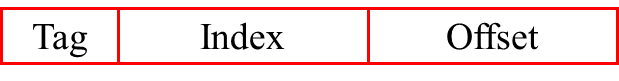
\includegraphics[width=0.5\textwidth]{images/memory_address.png}
    \caption{Memory Address Breakdown}
    \label{fig:memory_address}
\end{figure}
A cache can be broadly divided into two parts -cache directory which keep track of the address and information about whether the data is valid or not and the cache ram which actually stores the data. The cache is composed of multiple \textbf{sets}, where each set contains one or more \textbf{cache lines} (also called \textit{slots}). A cache line typically includes the following components:
\begin{itemize}
    \item \textbf{Tag:} A portion of the memory address used to verify if the data stored in the cache line corresponds to the requested address.
    \item \textbf{Valid Bit:} Indicates whether the data in the cache line is valid (i.e., whether it contains up-to-date information from main memory).
    \item \textbf{Data Block:} The actual data fetched from main memory.
\end{itemize}
It's schematic is as shown in the figure~\ref{fig:cache_memory}
\begin{figure}[H]
    \centering
    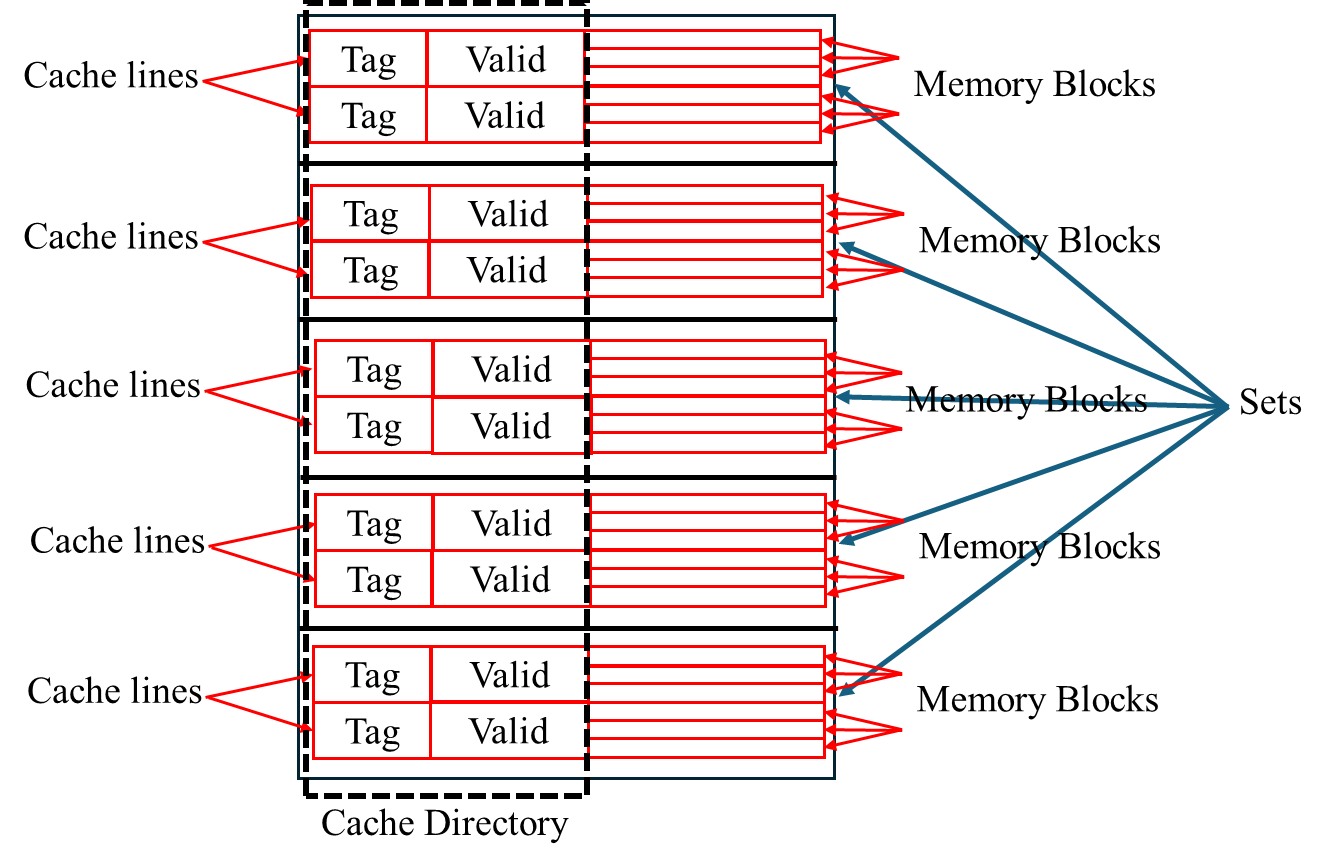
\includegraphics[width=0.8\textwidth]{images/cache_memory.png}
    \caption{Cache Memory}
    \label{fig:cache_memory}
\end{figure}

Main memory is organized into blocks or words, and cache memory is used to store a subset of these blocks for faster access. The cache is divided into small storage units called \textbf{cache lines} (or slots). Each cache line can hold exactly one block of data from the main memory. The process of deciding which cache line should hold which memory block is called \textbf{mapping}. Thus, ``mapping" refers to the rule that assigns a memory block to a particular cache line based on the memory address.

When a memory access occurs, the cache operates as follows:
\begin{enumerate}
    \item The \textbf{index} field is used to locate the appropriate cache set.
    \item Within the identified set, each cache line's tag is compared to the \textbf{tag} field of the memory address.
    \item If the tag matches and the \textbf{valid bit} is set, it results in a \textbf{cache hit}, and the data is fetched using the offset.
    \item If the tag does not match any line in the set, it results in a \textbf{cache miss}, and the data must be fetched from main memory.
\end{enumerate}
This is as illustrated in figure~\ref{fig:cache_lookup}
\begin{figure}
    \centering
    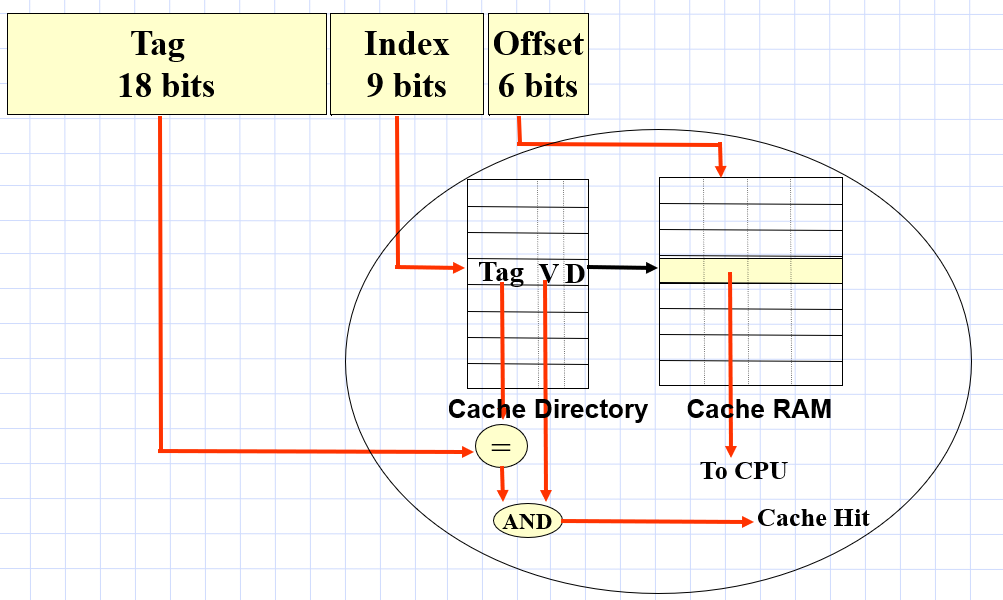
\includegraphics[width=0.7\linewidth]{images/mem_access.png}
    \caption{Cache Lookup and Access}
    \label{fig:cache_lookup}
\end{figure}
\begin{example}
Suppose a memory address is 16 bits long and the cache has 64 lines. Then, we need $\log_2 64 = 6$ bits to index the cache lines. These 6 bits are extracted from the memory address and used to determine which cache line the block maps to. So, memory blocks whose addresses share the same 6 index bits will always map to the same cache line.
\end{example}

The structure and number of sets and lines determine the type of cache organization (e.g., direct-mapped, set-associative, or fully associative, or even $m$-way set-associative), which will be discussed in subsequent sections.

\subsection{Direct-Mapped Cache}
In a \textbf{direct-mapped cache}, each cache set contains exactly \textbf{one cache line}. 


\subsubsection*{Cache Access Mechanism}
When the processor needs to access a memory word (instruction or data), it sends the corresponding memory address to the cache. The following steps occur:

\begin{enumerate}
    \item \textbf{Indexing:} The index bits of the memory address are used to determine the set (or cache line, in the case of direct-mapped cache) where the memory block might reside. This can be done very fast since the index bits refer to an address which can be located very easily.
    
    \item \textbf{Tag Comparison:} The remaining significant bits bits of the memory address, called the \emph{tag}, are compared with the tag stored in the selected cache line. Since there is only one cache line in each set, the index bits map to the cache lines directly.
    
    \item \textbf{Valid Bit Check:} Along with the tag, each cache line stores a valid bit indicating whether the data in the cache line is meaningful. If the valid bit is set and the tags match, a \textbf{cache hit} occurs.
    
    \item \textbf{Cache Hit:} If there is a match and the valid bit is set, the data is fetched directly from the cache, which is very fast compared to main memory access.
    
    \item \textbf{Cache Miss:} If the valid bit is not set or the tags do not match, a \textbf{cache miss} occurs. In this case:
    \begin{itemize}
        \item The processor fetches the required memory block from the main memory.
        \item In direct-mapped cache since each cache set contains exactly one cache line. This means that every memory block can map to exactly \emph{one} cache line in the cache. The specific line is determined using the \emph{index bits} of the memory address. These index bits identify which cache set the memory block corresponds to. Thus, a given memory block from main memory always maps to a single fixed location in the cache. If two memory blocks happen to have the same index bits, they will compete for the same cache line. When one is loaded, the other is evicted. This situation is known as a \textbf{conflict miss} and is a known limitation of direct-mapped caches. Thus, the fetched block is stored in the cache line corresponding to the index, replacing the existing block if any.
        \item The tag and valid bit of the cache line are updated.
        \item The processor resumes execution with the now-available data.
    \end{itemize}
    
\end{enumerate}

\paragraph{Advantages of Direct-Mapped Cache:}
\begin{itemize}
    \item Very simple to implement in hardware.
    \item Fast lookup due to one-to-one mapping.
    \item Less hardware cost compared to other mapping schemes.
\end{itemize}

\paragraph{Disadvantages of Direct-Mapped Cache:}
\begin{itemize}
    \item High chance of conflict misses. Two memory blocks in main memory that map to the same cache line will replace each other frequently.
    \item Poor utilization of cache space if many blocks compete for the same line.
\end{itemize}

Direct-mapped caches are efficient and fast, but the rigid mapping can lead to performance issues if many memory blocks map to the same cache line.

\subsection{Fully Associative Cache}
\label{sec:fully-associative-cache}

In a \textbf{fully associative cache}, any memory block can be stored in any cache line. It can be thought as only one cache set having all the cache lines. There is no fixed mapping between memory addresses and cache lines. So, there are no index bits in the address.

\subsubsection*{Cache Access Mechanism}
When the processor needs to access a data word or an instruction, it sends the memory address to the cache. The cache performs the following steps:

\begin{enumerate}
    \item \textbf{Tag Comparison – Associative Search:}  
    The memory address is divided into two parts: the \textbf{tag} and the \textbf{block offset}. Since any block can go into any cache line, there is no need for index bits.  
    The cache controller compares the tag of the incoming address with the tags of all cache lines in parallel. This is called an \textit{associative search}.

    \item \textbf{Valid Bit Check:}  
    Each cache line has a valid bit. It tells whether the content of the cache line is meaningful.  
    If the valid bit is set and the tag matches, we have a \textit{cache hit}.

    \item \textbf{Cache Hit:}  
    If there is a tag match and the valid bit is set, the required data is present in the cache. The data is directly sent to the processor. This access is much faster than going to the main memory.

    \item \textbf{Cache Miss:}  
    If there is no matching tag or the valid bit is not set, it results in a \textit{cache miss}. In this case:
    \begin{itemize}
        \item The required memory block is fetched from the main memory.
        \item The block is then placed into an available cache line.
        \item If all lines are full, one of the existing blocks is replaced using a \textit{replacement policy}. Common policies include:
        \begin{itemize}
            \item \textbf{FIFO (First-In-First-Out)}: Replace the oldest block.
            \item \textbf{LRU (Least Recently Used)}: Replace the block that was not used for the longest time.
            \item \textbf{Random}: Replace a randomly chosen block.
        \end{itemize}
        \item The tag and valid bit of the chosen cache line are updated.
        \item The processor resumes execution using the newly fetched data.
    \end{itemize}
\end{enumerate}

\subsubsection*{Advantages of Fully Associative Cache}
\begin{itemize}
    \item Very flexible. Any memory block can go into any cache line.
    \item Conflict misses are minimized, as blocks are not restricted to a fixed location.
\end{itemize}

\subsubsection*{Disadvantages of Fully Associative Cache}
\begin{itemize}
    \item Hardware is more complex. The cache must compare the incoming tag with all tags in parallel.
    \item Associative search uses more power and is slower than simple indexing.
    \item Cache access time is usually longer compared to a direct-mapped cache.
\end{itemize}



\subsection{Set Associative Cache}
\label{sec:set-associative-cache}

Set associative mapping is a hybrid between direct-mapped and fully associative caches. In this approach, the cache is divided into multiple \textbf{sets}. A $m$-way set associative means each set contains $m(>1)$ number of cache lines, also called \textit{ways}. A block of main memory maps to exactly one set, but it can go into any line within that set.

For example, consider a 4-way set-associative cache with 128 total cache lines. This means we have:
\[
\frac{128}{4} = 32 \text{ sets}
\]
Each set has 4 lines. A memory block is first mapped to a set using a portion of its address — typically using a modulo operation as shown in the figure~\ref{fig:set_associative} for a 2-way set-associative. Then, the block can be stored in any of the 4 lines within that set.

\begin{figure}[H]
    \centering
    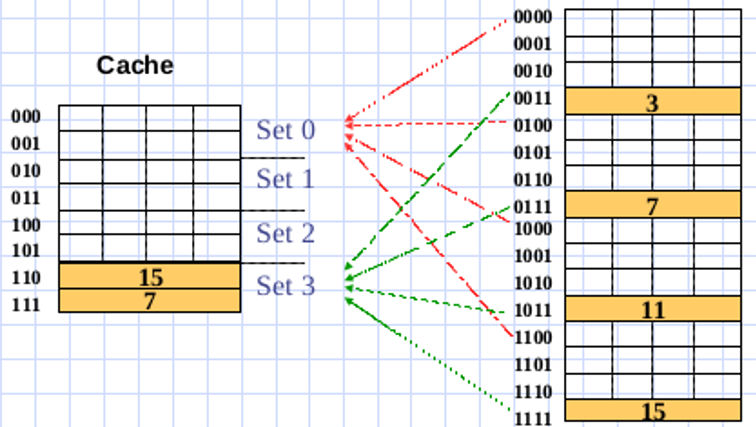
\includegraphics[width=0.5\linewidth]{images/set_associative.png}
    \caption{Set Associative Mapping}
    \label{fig:set_associative}
\end{figure}

\subsubsection*{Cache Access Mechanism}

When the processor needs to access a data word or an instruction, it sends the memory address to the cache. The following steps occur:

\begin{enumerate}
    \item \textbf{Indexing:}  
    The index bits from the memory address determine which set to look into. This is a fast and simple operation. It is similar to the indexing used in direct-mapped caches.

    \item \textbf{Tag Comparison (Associative Search within Set):}  
    The remaining significant bits of the address form the \textbf{tag}. The cache controller compares this tag with the tags of all cache lines inside the selected set. All lines in the set are checked in parallel.

    \item \textbf{Valid Bit Check:}  
    Each line in the set stores a valid bit. If the valid bit is set and the tag matches, the cache reports a \textbf{hit}.

    \item \textbf{Cache Hit:}  
    If a match is found, the data is fetched directly from the cache. This is much faster than accessing the main memory.

    \item \textbf{Cache Miss:}  
    If no matching tag is found or the valid bit is not set, a \textbf{miss} occurs. In that case:
    \begin{itemize}
        \item The memory block is fetched from the main memory.
        \item The block is placed into the corresponding set.
        \item If there is space (a line with invalid bit), the block is placed there.
        \item If all lines are occupied, one block is replaced using a replacement policy like:
        \begin{itemize}
            \item \textbf{FIFO (First-In-First-Out)}: Replace the oldest block.
            \item \textbf{LRU (Least Recently Used)}: Replace the least recently accessed block.
            \item \textbf{Random}: Replace a randomly chosen block.
        \end{itemize}
        \item The tag and valid bit are updated, and the processor resumes using the fetched data.
    \end{itemize}
\end{enumerate}
\begin{figure}[ht]
    \centering
    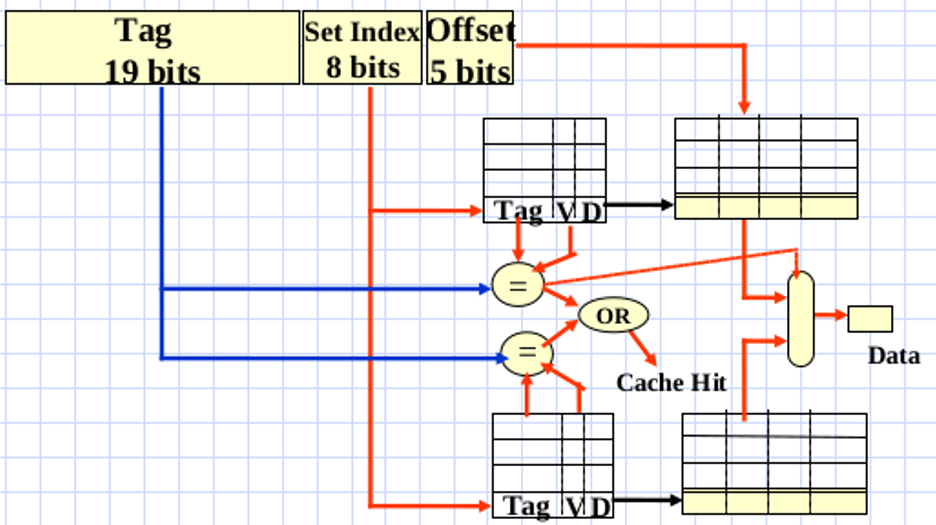
\includegraphics[width=0.7\linewidth]{images/2way_set.png}
\end{figure}
\subsubsection*{Advantages}
\begin{itemize}
    \item Reduces conflict misses compared to direct-mapped caches.
    \item More flexible than direct-mapped, but less complex than fully associative.
    \item Provides a good balance between speed, flexibility, and hardware cost.
\end{itemize}

\subsubsection*{Disadvantages}
\begin{itemize}
    \item Slightly slower than direct-mapped due to the parallel tag comparisons within each set.
    \item Requires more complex hardware than direct-mapped caches.
    \item Needs a replacement policy to decide which block to evict on a miss.
\end{itemize}

\begin{example}
Consider an example of an $8$ GB main memory (RAM). Let the size of each memory block be $64$ bytes and consider a typical cache size of $64$ KB, and assume a \textbf{2-way set-associative} mapping.

Since $8$ GB $\approx 2^{33}$ bytes, we need $33$ bits to uniquely identify each byte in memory (because $\log_2 2^{33} = 33$). Since the size of each memory block is $2^{64}$ bytes, which is $2^6$ bytes. Therefore, the total number of memory blocks in main memory is:
\[
    \frac{2^{33}}{2^6} = 2^{27}
\]
So, there are approximately $125 \times 10^6$ memory blocks.

To address these blocks, we need $27$ bits (since $\log_2 2^{27} = 27$). The remaining $6$ bits are used to specify the offset (i.e., the byte position) within a block.

Thus, each $33$-bit memory address can be divided as follows:
\begin{itemize}
    \item $27$ bits for the \textbf{block number}
    \item $6$ bits for the \textbf{offset} within the block
\end{itemize}

Since each memory block is $64$ bytes, each cache block is also $64$ bytes. In a 2-way set-associative cache, each \textbf{set} contains 2 blocks, meaning each set occupies $2 \times 64 = 128$ bytes.

So, the total number of sets in the cache is:
\[
    \frac{64 \text{ KB}}{128 \text{ bytes}} = \frac{2^{16}}{2^7} = 2^9 = 512 \text{ sets}
\]
Hence, we require $\log_2 512 = 9$ bits to index the cache sets.

Now recall that we need $27$ bits to address a memory block (from earlier). In set-associative mapping, the \textbf{least significant} $9$ bits of the block number are used as the \textbf{index} into the cache. The \textbf{remaining} $18$ bits serve as the \textbf{tag}, which is stored in the tag directory to check if a block is present in a set.

Finally, we still need the $6$ offset bits to identify the specific byte within the block.

Therefore, the 33-bit memory address is divided into:
\begin{itemize}
    \item \textbf{18 tag bits} (for block identification)
    \item \textbf{9 index bits} (for set selection)
    \item \textbf{6 offset bits} (for byte within block)
\end{itemize}

When the processor wants to access some data or an instruction, it sends a 33-bit memory address. This address is first searched in the cache. This also depends on the type of mapping associated with cache.

Since we are using a 2-way set associative cache, each cache set has 2 cache lines. The cache uses some bits of the memory address sent by the processor (called \textbf{index bits}) to find the correct set. Once the set is located, the cache compares the \textbf{tag bits} of the address with the tags stored in the two cache lines of that set. If there is a match, and the \textbf{valid bit} is set, it is a \textbf{cache hit}. This means the data is already in the cache and is sent to the processor. If there is no match, or the valid bit is not set, it is a \textbf{cache miss}. The data must then be fetched from the main memory and placed into one of the cache lines in that set.

In the case of a \textbf{cache miss}, the data or instruction requested by the processor must be fetched from the main memory and placed into the cache. Since the size of cache memory is limited, an existing memory block currently in the cache must be evicted to make room for the newly fetched block. The strategy used to determine which cache line gets replaced is called the \textbf{cache replacement policy}. In an $2$-way \textbf{set-associative cache}, the memory block is mapped to a cache set based on the index bits, and it can replace any of the $2$ cache lines within that set. Again, policies like FIFO or LRU are used to decide which of the $2$ lines in the set will be evicted and replaced by the new block. This design offers a trade-off between the high flexibility of a fully associative cache and the simple implementation of a direct-mapped cache.
\end{example}

\begin{example}
The table below gives the parameters for a number of different caches. For each cache, determine $S$, $t$, $s$, and $b$.

\begin{center}
\begin{tabular}{|c|c|c|c|c|c|c|c|c|}
    \hline
    Cache & $m$ & $C$ & $B$ & $E$ & $S$ & $t$ & $s$ & $b$ \\
    \hline
    1 & 32 & 1024 & 4  & 256 & \textcolor{blue}{1}  & \textcolor{blue}{30} & \textcolor{blue}{0} & \textcolor{blue}{2} \\
    \hline
    2 & 32 & 1024 & 8  & 128 & \textcolor{blue}{1}  & \textcolor{blue}{29} & \textcolor{blue}{0} & \textcolor{blue}{3} \\
    \hline
    3 & 32 & 1024 & 32 & 32  & \textcolor{blue}{1}  & \textcolor{blue}{27} & \textcolor{blue}{0} & \textcolor{blue}{5} \\
    \hline
    4 & 32 & 1024 & 32 & 2   & \textcolor{blue}{16} & \textcolor{blue}{23} & \textcolor{blue}{4} & \textcolor{blue}{5} \\
    \hline
\end{tabular}
\end{center}

\vspace{1em}
\textbf{Explanation for Cache 1:}

Given:
\begin{itemize}
    \item $m = 32$, $C = 1024$ bytes, $B = 4$ bytes, $E = 256$
\end{itemize}

Then:
\begin{itemize}
    \item Total blocks $= \frac{C}{B} = \frac{1024}{4} = 256$
    \item Number of sets $S = \frac{C}{B\cdot E} = \frac{256}{256} = 1$
    \item Block offset bits $b = \log_2 B = \log_2 4 = 2$
    \item Set index bits $s = \log_2 S = \log_2 1 = 0$
    \item Tag bits $t = m - s - b = 32 - 0 - 2 = 30$
\end{itemize}

The same formulas can be used for the other entries.
\end{example}


\begin{note}
    Note that in this section, we have not gone into the nitty-gritty details of how cache works internally or how it is managed by the system. We have skipped several important topics such as write strategies (like write-through and write-back), cache coherence in multi-core systems, and the structure of real-world cache hierarchies (like L1, L2, and L3 caches). Our goal here was to give a high-level understanding of what a cache is and how it helps speed up memory access. We will revisit some of these advanced topics later in the book if needed. For a deeper explanation, refer to the book~\cite{bryant2016computer}.
\end{note}

\section{Cache and Programming}
In this section, we will learn how cache-related performance issues can affect important parts of our programs. We will also look at some simple examples to understand this better. 

For simplicity, we will focus only on the \textbf{data cache}, assuming that instruction and data caches are separate. Let the memory address be of $32$ bits. The configuration of the data cache we will be working with is as follows:
\begin{itemize}
    \item Cache type: Direct-mapped
    \item Cache size: 16 KB
    \item Block size: 32 Bytes
\end{itemize}

Since the cache is direct-mapped with a total size of 16 KB and a block size of 32 Bytes, it contains:
\begin{itemize}
    \item $\frac{16 \times 1024}{32} = 512$ cache lines (or sets because of direct-mapped cache)
    \item Thus, $\log_2 512 = 9$ index bits,
    \item and $\log_2 32 = 5$ block offset bits
    \item The remaining $18$ bits will be the tag bits.
\end{itemize}
\subsection{Example 1: Vector Sum Reduction}

We are interested in computing a scalar value that reduces a vector by summing all its elements. This requires a loop that adds each element of the vector to an accumulator.

\begin{lstlisting}[style=cppstyle, caption={Vector Sum Reduction}]
double A[2048], sum = 0.0;
for (i = 0; i < 2048; i++) sum = sum + A[i];
\end{lstlisting}

In this example, the array \texttt{A} contains 2048 double-precision values, with each value occupying $8$ bytes (64-bit format). The variable \texttt{sum} is also of type \texttt{double}, and thus occupies $8$ bytes.

The loop iterates through all the elements of the array, adding each value of \texttt{A[i]} to the \texttt{sum} variable. This is a simple example of a vector reduction operation, often used in numerical computations.

To analyze cache behavior, we must examine the program at a level close to machine code to identify memory load and store operations. Specifically, we want to determine which memory accesses occur and in what order, given our data cache configuration—a direct-mapped 16KB cache with 32-byte block size.

For simplicity, we assume that the variables \texttt{i} and \texttt{sum} reside in registers. This is a reasonable assumption, as we can ensure that these variables are kept in registers by the compiler or through manual optimization. As a result, they do not involve memory accesses and therefore do not impact cache performance.

Hence, we will focus only on memory accesses to the array \texttt{A}, since it is the only data structure being read from memory in the loop. Therefore, analyzing the vector sum reduces to understanding what happens when accessing \texttt{A[0]}, \texttt{A[1]}, ..., up to \texttt{A[2047]}. We will now examine how this sequential access translates into memory operations:
\begin{itemize}
    \item Each element \texttt{A[i]} (for $i = 0$ to $2047$) must be loaded from memory into a CPU register. Here, a \textbf{load} refers to an instruction that copies data from main memory into a register. Once in a register, the value can be added to the \texttt{sum} variable.
    
    \item To proceed with the analysis, we assume that the base address of the array \texttt{A} (i.e., the address of \texttt{A[0]}) is \texttt{0xA000}, which corresponds to the binary address \texttt{10101000000000000}, with all more significant bits set to zero.
    
    \item Since our cache is 16KB (i.e., $2^{14}$ bytes) with a block size of 32 bytes (i.e., $2^5$), the cache is divided into $2^9 = 512$ blocks. So, we need 9 index bits and 5 offset bits. We’ll analyze cache behavior by tracking how these 14 bits (9 index + 5 offset) change as the array is accessed sequentially.
    
    \item The index bits for \texttt{A[0]} are \texttt{100000000} (which is decimal 256). So \texttt{A[0]} will map to cache index 256.
    
    \item Since the array elements are of type \texttt{double}, each occupies 8 bytes. A 32-byte block can thus hold 4 consecutive elements: \texttt{A[0]}, \texttt{A[1]}, \texttt{A[2]}, and \texttt{A[3]}.
    
    \item So, when there’s a cache miss for \texttt{A[0]}, the entire block containing \texttt{A[0]} through \texttt{A[3]} is brought into the cache. That means subsequent accesses to \texttt{A[1]}, \texttt{A[2]}, and \texttt{A[3]} will be cache hits.
    
    \item The next miss happens at \texttt{A[4]}, which maps to index 257. But again, a full block containing \texttt{A[4]} to \texttt{A[7]} is loaded. So \texttt{A[5]}, \texttt{A[6]}, and \texttt{A[7]} will hit in cache.
    
    \item This pattern continues — every 4th access is a miss (cold miss), and the next three accesses are hits due to spatial locality.
\end{itemize}

We now analyze this behavior assuming the cache is initially empty, which is also known as a \textbf{cold start}. The first access to each block (like \texttt{A[0]}, \texttt{A[4]}, \texttt{A[8]}, etc.) causes a cache miss, but the next three accesses within that block are cache hits. 

So, in total, there are $2048 / 4 = 512$ cache misses (one for every block of 4), and $2048 - 512 = 1536$ cache hits. This gives us a \textbf{hit ratio} of:
\[
\frac{1536}{2048} = 0.75 \quad \text{or} \quad 75\%
\]
This performance gain comes entirely from \textbf{spatial locality} — because we're accessing data laid out consecutively in memory.

Now suppose we add a loop before the reduction to preload all relevant memory blocks:
\begin{lstlisting}[style=cppstyle, caption={Preloading the Array for Temporal Locality}]
for (i = 0; i < 2048; i++) tmp = A[i]; // preload
double A[2048], sum = 0.0;
for (i = 0; i < 2048; i++) sum = sum + A[i];
\end{lstlisting}

With this change, the second loop sees a \textbf{100\% hit ratio}. This is because:
\begin{itemize}
    \item $75\%$ of hits come from \textbf{spatial locality} (within each block), and
    \item $25\%$ of hits come from \textbf{temporal locality}, since the data was already loaded in the first loop and hasn't been evicted.
\end{itemize}

Suppose now the array is defined as \texttt{double A[4096]}. Will this make any difference? Consider the case where the loop is preceded by another loop that accesses all array elements in sequential order. The total memory required to store the array is $8 \times 4096 = 32$~KB, while the cache memory is only 16~KB. Hence, the entire array cannot fit into the cache. After execution of the previous loop, the second half of the array will be in the cache and because of the spatial locality of reference it is anyways not going to be used for vector sum. This is just wasting time due to unnecessary memory accesses to no advantage. As a result, our loop will still experience cache misses, just as we analyzed earlier.

Recall that to estimate the data cache hit rate, we made the following assumptions:
\begin{itemize}
    \item The variables \texttt{sum} and \texttt{i} are stored in registers; hence, we ignore their memory accesses.
    \item The base address of \texttt{A[0]} is assumed to be \texttt{0xA000}.
    \item We consider that only load/store instructions access memory operands; all other instructions use register operands.
\end{itemize}

\subsection{Example 2: Vector Dot Product}
In this case, we are interested in computing the dot product (also called the inner product) between two vectors, $A$ and $B$, represented by the arrays \texttt{A} and \texttt{B}. The dot product is computed by taking the running sum of the products of corresponding elements from the two arrays. 

As in the previous example, we will assume similar conditions and ignore the accesses to the loop index variable \texttt{i} and the variable \texttt{sum}, assuming they are stored in registers. Also, we will assume that only load/store instructions access memory operands; all other instructions use register operands.

\begin{lstlisting}[style=cppstyle, caption={Vector Dot Product}]
double A[2048], B[2048], sum = 0.0;
for (i = 0; i < 2048; i++) 
    sum = sum + A[i] * B[i];
\end{lstlisting}

We are interested in analyzing the order of reference sequence, which will be: \texttt{load A[0]}, \texttt{load B[0]}, and so on, till \texttt{load A[2047]}, \texttt{load B[2047]}.

We now assume the base addresses of arrays $A$ and $B$ as $0xA000$ and $0xE000$ respectively. Since these arrays are declared as \texttt{double}, each element occupies $8$ bytes, and therefore, $4$ consecutive elements of the array will fit into each $32$-byte cache block.

Now, $0xA000$ in binary is $1010\ 0000\ 0000\ 0000$, which corresponds to cache index $256$. Similarly, $0xE000$ in binary is $1110\ 0000\ 0000\ 0000$, which also maps to the same index $256$.

Because the index bits are the same, both $A[0]$ and $B[0]$ will be loaded into the same cache set (index $256$). This leads to a problem: consider the load sequence. When we first load $A[0]$, there is a cache miss (a cold miss, assuming the cache is initially empty) at cache set index $256$. Thus, it loads $A[0] A[1], A[2], A[3]$ into the cache set memory block. Next, when we load $B[0]$, it maps to the same cache set index and causes another miss — this time a conflict miss, because it replaces the block holding $A[0]$.

A conflict miss occurs when multiple memory blocks map to the same cache set and compete for space under a direct-mapped cache scheme. In this case, since $A[0]$ and $B[0]$ conflict with each other, loading $B[0]$ causes memory block containing $A[0], A[1], A[2], A[3]$ to be evicted and load $B[0], B[1], B[2], B[3]$ into the cache set memory block. Now, when \texttt{load A[1]} is executed, it again maps to the same cache set (index $256$), and because it is not in the cache (recall the memory block containing $A[0], A[1], A[2], A[3]$ was evicted), we get yet another cache miss.

This process continues, resulting in a conflict miss for every access, significantly reducing cache efficiency. Thus, the hit ratio for our program is $0\%$. The source of the problem is that the elements of arrays $A$ and $B$ are accessed in order and both map to the same cache index. As a result, each new access causes the previous entry to be evicted, leading to no cache reuse. The hit ratio would have been better if the base address of array $A$ had been different from that of array $B$, such that the memory blocks mapped to different cache set indices. This would have prevented the conflicts and improved the cache performance.

The question now is: was this a contrived example? The root cause of the problem was that we assumed the base addresses of arrays $A$ and $B$ to be $0xA000$ and $0xE000$, respectively, such that both mapped to the same cache set index. Is this an unreasonable assumption that never occurs in the real world? The answer is no—it is not an unreasonable assumption. In fact, this behavior is consistent with the memory allocation model typically followed by compilers.

To understand this better, we must ask: how are variable addresses assigned by the compiler? Typically, the compiler begins allocating memory from a starting address, which is often outside the programmer’s control. Suppose, for instance, that the compiler begins by placing array $A$ at address $0xA000$. It then assigns memory to subsequent variables in the order they are declared. Since array $A$ consists of $2048$ elements of type \texttt{double} (each 8 bytes), the total space it occupies is $2048 \times 8 = 16384$ bytes, or $0x4000$ in hexadecimal. Therefore, array $B$ will be placed at address $0xA000 + 0x4000 = 0xE000$.

\[
\text{Address of } B = 0xA000 + 2048 \times 8 = 0xA000 + 0x4000 = 0xE000
\]
\[
\text{Binary: } 1010\ 0000\ 0000\ 0000 + 0100\ 0000\ 0000\ 0000 = 1110\ 0000\ 0000\ 0000
\]

Thus, both arrays may end up mapping to the same cache set index, causing conflict misses, even though this layout results naturally from how compilers assign addresses in practice.

Thus, the problem arises due to the nature of the cache hardware and the specific issue caused by the vector size of $2048$. The compiler typically assigns addresses to variables in the order they are declared.

Our objective is therefore to shift the base address of array $B$ just enough so that the cache index of $B[0]$ differs from that of $A[0]$:
\begin{lstlisting}[style=cppstyle]
double A[2052], B[2048];
\end{lstlisting}

Now, the base address of $B$ would be
\[
0xA000 + 2052 \times 8 = 0xE020,
\]
which corresponds to a cache index of $257$. Hence, $B[0]$ and $A[0]$ no longer conflict for the same cache block. The resulting hit ratio will rise to \textbf{75\%}. 

This is a common optimization trick used in languages like \textbf{Fortran}. By doing so, we have improved the cache hit ratio—but what impact does this have on the execution time of the program?

Suppose the following piece of code is a dominant part of the program, i.e., its performance heavily influences the overall execution time. Let us now analyze the number of cycles required for execution.

Assume there are $20$ machine instructions inside the loop: $2$ load instructions and $18$ others (such as additions, register loads, and loop overhead), which do not access memory and thus take only $1$ cycle per instruction. The total number of instructions executed is therefore $20 \times 2048$.

Assume each instruction takes $1$ cycle to execute, and a load miss incurs a penalty of $100$ cycles to fetch the data from memory.

\begin{itemize}
    \item \textbf{Best Case (100\% hit ratio):}  
    All instructions take only $1$ cycle. Thus, total cycles =  
    \[
    20 \times 2048 = 40960 \text{ cycles}.
    \]
    
    \item \textbf{Worst Case (0\% hit ratio):}  
    All $18$ non-load instructions take $1$ cycle each. The $2$ load instructions take $100$ cycles each due to cache misses. Thus, the total number of cycles is  
    \[
    (18 \times 1 + 2 \times 100) \times 2048 = (18 + 200) \times 2048 = 446464 \text{ cycles}.
    \]
    
    \item \textbf{Intermediate Case (75\% hit ratio):}  
    $75\%$ of the loads are cache hits (taking $1$ cycle), and $25\%$ are misses (taking $100$ cycles). So the load-related cycles are  
    \[
    0.75 \times 2048 \times 2 \times 1 + 0.25 \times 2048 \times 2 \times 100 = 3072 + 102400.
    \]
    The remaining $18$ instructions per iteration (which are not memory loads) always take $1$ cycle:  
    \[
    18 \times 2048 = 36864.
    \]
    Hence, the total number of cycles is  
    \[
    3072 + 102400 + 36864 = 142336 \text{ cycles}.
    \]
\end{itemize}

Thus, we observe that a better cache hit ratio significantly reduces the execution time—improving performance by almost a factor of $3$ compared to the $0\%$ hit case, and closing the gap toward the ideal case.


Another method is called \textbf{Array Merging}, where we merge the arrays $A$ and $B$ together, as shown in the following code:

\begin{lstlisting}[style=cppstyle]
struct {double A, B;} array[2048];
for (i = 0; i < 2048; i++) 
    sum += array[i].A * array[i].B;
\end{lstlisting}

The nature of the dot product remains the same, but now it picks two elements from the same array element of the newly defined structure. The idea is that spatial locality of reference will help here because the compiler will store \texttt{A[i]} and \texttt{B[i]} adjacent in memory since they are part of the same \texttt{struct}. 

Of course, in many programs, such a redefinition might not be possible, because \texttt{A} and \texttt{B} may have distinct meanings or uses in the calculations being performed, and it may not always be feasible to restructure the data in this way.

In this method, the hit ratio will again be $75\%$ because each cache block will now contain \texttt{A[0]}, \texttt{B[0]}, \texttt{A[1]}, \texttt{B[1]}, and so on. Thus, the first access to \texttt{A[0]} will be a cache miss due to a cold start, but the accesses to \texttt{B[0]}, \texttt{A[1]}, and \texttt{B[1]} will be cache hits.

\subsection{Example 3: DAXPY}

We now consider another famous example called DAXPY (\textbf{D}ouble precision \textbf{AX} \textbf{P}lus \textbf{Y}), where $a$ is a scalar and $X$ and $Y$ are vectors.

\begin{lstlisting}[style=cppstyle, caption={Double precision AX Plus Y (DAXPY)}]
double X[2048], Y[2048], a;
for (i = 0; i < 2048; i++) 
    Y[i] = a * X[i] + Y[i];
\end{lstlisting}

This example differs slightly from the previous one, as there are three array references per iteration of the loop. Specifically, for each $i$, we must load \texttt{X[i]}, load \texttt{Y[i]}, and then store the updated value back to \texttt{Y[i]}. 

The reference sequence thus becomes: 
\begin{center}
\texttt{load X[0], load Y[0], store Y[0], load X[1], load Y[1], store Y[1],} $\dots$, \texttt{load X[2047], load Y[2047], store Y[2047]}
\end{center}

Assuming that the base addresses of arrays \texttt{X} and \texttt{Y} do not conflict in the cache, we can compute the hit ratio. In this case, out of every 12 memory references (two loads and one store per iteration), there will typically be 1 miss for \texttt{X[0]} and 1 miss for \texttt{Y[0]} due to cold starts. The remaining references will be cache hits assuming spatial locality is exploited effectively. Thus, the overall hit ratio is approximately $\frac{10}{12}\times 100 =  83.3\%$.

\subsection{Example 4: 2D Matrix Sum}
We will now look at the sum of two-dimensional matrices as shown below:

\begin{lstlisting}[style=cppstyle]
double A[1024][1024], B[1024][1024];
for (j = 0; j < 1024; j++)
    for (i = 0; i < 1024; i++)
        B[i][j] = A[i][j] + B[i][j];
\end{lstlisting}

This is somewhat similar to DAXPY, and the reference memory access sequence would be:  
\texttt{load A[0,0], load B[0,0], store B[0,0], load A[1,0], load B[1,0], store B[1,0],} and so on.

Before analyzing the cache hit rate, it is important to answer a more fundamental question:  
\textbf{In what order are the elements of a multidimensional array stored in memory?}

In the case of one-dimensional arrays, the elements are stored contiguously in memory. However, when dealing with two-dimensional matrices, we must ask whether the matrix is stored row by row (row-major order) or column by column (column-major order). Different programming languages make different assumptions regarding this.

Compilers implement address calculations for multidimensional arrays based on the language's assumed storage order. Therefore, to compile a program correctly in terms of memory load and store operations, the compiler must know how the language stores multidimensional arrays. It is assumed that the compiler already knows the language-specific storage convention. Otherwise, it would have to make its own assumptions, which could severely affect performance portability.

\textbf{Performance portability} refers to the idea that even if a program remains functionally correct across different compilers or languages, its performance may vary significantly depending on how the underlying compiler interprets the array storage order.

This storage order convention is a property of the language, not the compiler. The two common conventions are:

\begin{itemize}
    \item \textbf{Row-major order:}
    \begin{itemize}
        \item For a two-dimensional array, the elements of the first row are stored first, followed by the elements of the second row, then the third, and so on.
        \item This is the convention used in \texttt{C}.
    \end{itemize}
    
    \item \textbf{Column-major order:}
    \begin{itemize}
        \item For a two-dimensional array, the elements are stored column by column in memory.
        \item This is the convention used in \texttt{Fortran}.
    \end{itemize}
\end{itemize}
Now, we are assuming the programming language to be C. In C, multi-dimensional arrays are stored in \textbf{row-major order}, which means that elements like $A[0][0]$, $A[0][1]$, $A[0][2]$, and $A[0][3]$ are stored in adjacent memory locations, typically mapping to the same cache block. Therefore, the given program is written inefficiently. 

To understand this, consider the reference sequence: if we access $A[1][0]$ immediately after $A[0][0]$, these elements are stored in different rows and thus different cache blocks, resulting in a cache miss. This indicates poor \textbf{spatial locality}.

We observe a mismatch between the \textbf{reference order}—the order in which memory is accessed—and the \textbf{storage order}—the way memory is actually laid out. Our program steps through the matrix column by column, resembling \textbf{column-major order}, whereas C stores matrices in \textbf{row-major order}: $A[0][0]$, $A[0][1]$, and so on. As a result, our loop does not exploit spatial locality, although it does demonstrate some \textbf{temporal locality}, since the store operation to $B[0][0]$ immediately follows a load from $B[0][0]$, which remains in the cache.

Thus, the loop will not show any spatial locality. Here, we assume that packing has been done to eliminate conflict misses due to base addresses. However, in this case, it does not really matter, as there is no spatial locality anyway, and temporal locality will not be affected by conflict misses. So we get:
\begin{itemize}
    \item A miss on \texttt{load A[0][0]} (due to cold start),
    \item A miss on \texttt{load B[0][0]} (due to cold start),
    \item A hit on \texttt{store B[0][0]} (due to temporal locality),
\end{itemize}
Now, when we go to the next instruction \texttt{load A[1][0]}, we again get a miss (due to cold start), and so on. Thus, the hit ratio is approximately $33\%$, entirely because of the temporal locality—on the store instructions. There are no hits for the load instructions at all.

Will \texttt{A[0][1]} be in the cache when required later in the loop? 

Now let us analyze the impact of \textbf{loop interchange}. Recall that in the initial version of the loop, the second subscript was in the outer loop and the first subscript was in the inner loop. We now consider the interchanged version, where the first subscript is in the outer loop and the second subscript is in the inner loop, as shown below:

\begin{lstlisting}[style=cppstyle]
double A[1024][1024], B[1024][1024];
for (i = 0; i < 1024; i++)
    for (j = 0; j < 1024; j++)
        B[i][j] = A[i][j] + B[i][j];
\end{lstlisting}

In this case, the memory reference sequence would be:
\begin{itemize}
    \item \texttt{load A[0][0]}, \texttt{load B[0][0]}, \texttt{store B[0][0]}
    \item \texttt{load A[0][1]}, \texttt{load B[0][1]}, \texttt{store B[0][1]}
    \item $\dots$
\end{itemize}

We observe that the first time \texttt{A[0][0]} is loaded, it results in a cache miss due to a cold start. Similarly, \texttt{load B[0][0]} will also result in a cache miss. However, the subsequent \texttt{store B[0][0]} will be a cache hit, since the value was just loaded and remains in the cache. Similarly, \texttt{load A[0][1]} will likely be a cache hit as it resides in the same cache block as \texttt{A[0][0]}, assuming a typical cache line size of 4 words. The same applies to the accesses for \texttt{B[0][1]}, \texttt{store B[0][1]}, and so on.

Hence, out of the first 12 memory instructions (8 loads and 4 stores), 10 will be cache hits and only 2 will be cache misses. This leads to a cache hit rate of:
\[
\frac{10}{12} \times 100 = 83.3\%
\]
This improved hit rate demonstrates better \textbf{spatial locality} due to the access pattern now matching the row-major storage layout of C arrays.

This leads to an important question: is it always safe to perform loop interchange? Consider the following example, where the secondary subscript is controlled by the outer loop:

\begin{lstlisting}[style=cppstyle]
for (j = 1; j < 2048; j++)
    for (i = 1; i < 2048; i++)
        A[i][j] = A[i+1][j-1] + A[i][j-1];
\end{lstlisting}

This ordering is clearly incorrect since the second subscript, which denotes the column (i.e., `j`), is controlled by the outer loop. We have already discussed such cases previously. This example is trivial, but many numerical codes still fall into this trap. We are interested in the version where the `for` loops are interchanged, since we know that doing so can improve spatial locality.

Let us examine the actual behavior of this loop by tracing its first few iterations. For instance:
\[
A[1][1] = A[2][0] + A[1][0], \quad A[2][1] = A[3][0] + A[2][0], \quad \text{and so on}.
\]
Then, for the next column:
\[
A[1][2] = A[2][1] + A[1][1].
\]

Now let us blindly interchange the two `for` loops and observe the effect:

\begin{lstlisting}[style=cppstyle]
for (int i = 1; i < 2048; i++)  // interchanged
    for (int j = 1; j < 2048; j++)
        A[i][j] = A[i+1][j-1] + A[i][j-1];
\end{lstlisting}


With this ordering, the first few iterations will now be:
\[
A[1][1] = A[2][0] + A[1][0], \quad A[1][2] = A[2][1] + A[1][1], \quad \text{and so on,}
\]
until we reach:
\[
A[2][1] = A[3][0] + A[2][0].
\]

Notice the subtle but crucial difference. In the original loop nest, the computation of $A[1][2]$ used updated values of both $A[2][1]$ and $A[1][1]$. However, in the interchanged version, the value of $A[1][2]$ is computed using the old value of $A[2][1]$ (since `i = 2` has not yet been processed) and the updated value of $A[1][1]$. This changes the computation semantics and may lead to incorrect results.

Hence, \textbf{loop interchange is not always safe}, especially when data dependencies exist across loop iterations. One must carefully analyze the dependencies before performing such optimizations.

Is there any safer way to modify the loops so that the code remains correct while also achieving better spatial locality? The answer is yes. This can be accomplished by rewriting the loop to iterate over the second subscript from higher to lower values, as shown below:

\begin{lstlisting}[style=cppstyle]
for (i = 2047; i > 1; i--)
    for (j = 1; j < 2048; j++)
        A[i][j] = A[i+1][j-1] + A[i][j-1];
\end{lstlisting}

This transformation ensures that data accessed in close temporal proximity is also stored in adjacent memory locations, thus taking better advantage of spatial locality.

However, this example also illustrates an important principle: \textbf{loop interchange should not be applied blindly}. Instead, the loop structure should be carefully analyzed or modified to exploit the memory hierarchy effectively. Such strategies can be learned through experience, systematic experimentation, or by exploring various loop arrangements and identifying those that provide the best spatial locality of reference.

\subsection{Example 5: Matrix Multiplication}
Here is an example for matrix multiplication.
\begin{lstlisting}[style=cppstyle]
double X[N][N], Y[N][N], Z[N][N];
for(i=0;i<N;i++)
    for (j=0lj<N;j++)
        for(k=0;k<N;k++)
            X[i][j] += Y[i][k]*Z[k][j];
\end{lstlisting}
Assume that $N$ is a power of $2$. This is the basic form of matrix multiplication we usually learn in high school.

A common way to optimize it is to reduce the number of memory accesses. In the naive version, we access \texttt{X[i][j]} repeatedly in the innermost loop to update the running sum. This can be improved.

We can store the running sum in a temporary variable called \texttt{tmp}, and after the innermost loop finishes, we copy it into \texttt{X[i][j]}. This way, we access \texttt{X[i][j]} only once per iteration, which reduces the load/store pressure.

Here’s how the updated code looks:

\begin{lstlisting}[style=cppstyle, caption={Optimized Matrix Multiplication using temporary variable}, label={lst:opt-matmul}]
double X[N][N], Y[N][N], Z[N][N];
for (int i = 0; i < N; i++) {
    for (int j = 0; j < N; j++) {
        double tmp = 0.0; // Running sum
        for (int k = 0; k < N; k++) {
            tmp += Y[i][k] * Z[k][j]; // Dot product
        }
        X[i][j] = tmp;
    }
}
\end{lstlisting}

\textbf{Note:} We use \texttt{tmp} to hold the dot product of the $i^{\text{th}}$ row of $Y$ and $j^{\text{th}}$ column of $Z$.

This saves several memory references by avoiding frequent reads/writes to \texttt{X[i][j]}.

Let’s now observe how data is accessed during execution:

\begin{itemize}
    \item To compute \texttt{X[0][0]}, we load:
    \begin{itemize}
        \item \texttt{Y[0][0]}, \texttt{Z[0][0]}
        \item \texttt{Y[0][1]}, \texttt{Z[1][0]}
        \item \dots
        \item \texttt{Y[0][N-1]}, \texttt{Z[N-1][0]}
    \end{itemize}
    Then we store \texttt{X[0][0]}.

    \item To compute \texttt{X[0][1]}, we load:
    \begin{itemize}
        \item \texttt{Y[0][0]}, \texttt{Z[0][1]}
        \item \texttt{Y[0][1]}, \texttt{Z[1][1]}
        \item \dots
        \item \texttt{Y[0][N-1]}, \texttt{Z[N-1][1]}
    \end{itemize}
    Then we store \texttt{X[0][1]}.
\end{itemize}

And so on, row by row.

In this version of matrix multiplication (loop order \texttt{ijk}), the references to $Y$ happen row-wise: 
\texttt{Y[0][0]}, \texttt{Y[0][1]}, \dots, and so on. This means $Y$ shows excellent \textit{spatial locality of reference}, since successive elements in memory are accessed in sequence.

However, the references to $Z$ occur column-wise: \texttt{Z[0][0]}, \texttt{Z[1][0]}, \dots. This results in poor spatial locality for $Z$, since non-contiguous memory elements are accessed. 

Therefore, this version of the loop has good cache behavior for $Y$ but poor cache performance for $Z$.

\subsubsection*{Loop intercahnge}
Let us now explore the idea of \textbf{loop interchange} further. We can rearrange the three nested loops in any order without affecting the correctness of the program. That is, all permutations of the loop order (\texttt{ijk}, \texttt{jik}, \texttt{ikj}, etc.) compute the same result: the matrix product $X = Y \cdot Z$.

For example, we can interchange the $i$ and $k$ loops, resulting in the order \texttt{kji}, as shown below:

\begin{lstlisting}[style=cppstyle, caption={Matrix multiplication with loop order kji}, label={lst:kji-matmul}]
for (int k = 0; k < N; k++)
    for (int j = 0; j < N; j++){
        double tmp = 0.0;
        tmp = Z[k][j];
        for (int i = 0; i < N; i++)
            X[i][j] += Y[i][k] * tmp;
    }
\end{lstlisting}

In this version, observe that for each fixed pair $(k, j)$, the value \texttt{Z[k][j]} is reused for all $i$. So it can be loaded into a register once and reused across the innermost loop. This reduces the number of memory references to $Z$ significantly.

However, now the access pattern for $X$ and $Y$ becomes column-wise:
\begin{itemize}
    \item Load \texttt{X[0][0]}, load \texttt{Y[0][0]}, store \texttt{X[0][0]}
    \item Load \texttt{X[1][0]}, load \texttt{Y[1][0]}, store \texttt{X[1][0]}
    \item \dots
\end{itemize}

This means both $X$ and $Y$ are accessed in a non-contiguous (column-wise) fashion, which leads to poor spatial locality and a high number of cache misses.

So, although the number of loads for $Z$ is reduced, the cache behavior for $X$ and $Y$ becomes worse.

Thus, we see that there are 6 different possibilities for loop variants: $ijk$, $ikj$, $jik$, $jki$, $kij$, and $kji$. Each of them would be correct in computing the matrix multiplication but would have different cache efficiencies. We already saw the cache efficiencies of the $ijk$ and $kij$ loops. Now let us see the cache efficiencies for the other 4. For example, for $ikj$, the code would be as follows:

\begin{lstlisting}[style=cppstyle,caption={Matrix multiplication with loop order ikj}, label={lst:ikj-matmul}]
for (int i = 0; i < N; i++)
    for (int k = 0; k < N; k++) {
        double tmp = Y[i][k];
        for (int j = 0; j < N; j++)        
            X[i][j] += tmp * Z[k][j];
    }
\end{lstlisting}

Here, we see that the reference sequence would be: load \texttt{X[0][0]}, load \texttt{Z[0][0]}, store \texttt{X[0][0]}, load \texttt{X[0][1]}, load \texttt{Z[0][1]}, store \texttt{X[0][1]} and so on. Thus, we see that $X$ and $Z$ are accessed in a row-wise manner. Therefore, this would have excellent spatial locality for both $X$ and $Z$.

Now let us consider the $jik$ loop order. The corresponding code is:

\begin{lstlisting}[style=cppstyle,caption={Matrix multiplication with loop order jik}, label={lst:jik-matmul}]
for (int j = 0; j < N; j++)
    for (int i = 0; i < N; i++) {
        double tmp = 0.0;
        for (int k = 0; k < N; k++)
            tmp += Y[i][k] * Z[k][j];
        X[i][j] += tmp;
    }
\end{lstlisting}

Here, we see that the reference sequence would be: load \texttt{Y[0][0]}, load \texttt{Z[0][0]}, load \texttt{Y[0][1]}, load \texttt{Z[1][0]}, and so on. The matrix $Y$ is accessed row-wise, and $Z$ is accessed column-wise. After computing the inner loop, we write to \texttt{X[0][0]}.

So, in this case, $Y$ has good spatial locality since it is accessed row-wise. But $Z$ is accessed column-wise and hence shows poor spatial locality. The write to $X[i][j]$ happens once per $(i,j)$, so it is fine.

Thus, this loop order has good cache performance for $Y$, but poor cache behavior for $Z$.
 
Now let us consider the $jki$ loop order. The corresponding code is:

\begin{lstlisting}[style=cppstyle,caption={Matrix multiplication with loop order jki}, label={lst:jki-matmul}]
for (int j = 0; j < N; j++)
    for (int k = 0; k < N; k++) {
        double tmp = Z[k][j];
        for (int i = 0; i < N; i++)
            X[i][j] += Y[i][k] * tmp;
    }
\end{lstlisting}

Here, we see that the reference sequence would be: load \texttt{X[0][0]}, load \texttt{Y[0][0]}, store \texttt{X[0][0]}, load \texttt{X[1][0]}, load \texttt{Y[1][0]}, store \texttt{X[1][0]}, and so on. So, we observe that both $X$ and $Y$ are accessed column-wise, while $Z[k][j]$ is loaded once per inner loop and reused.

Thus, this version shows good reuse of $Z$ due to register storage, but has poor spatial locality for both $X$ and $Y$ because they are accessed column-wise. Therefore, this loop order results in many cache misses for $X$ and $Y$.

Now let us consider the $kij$ loop order. The corresponding code is:

\begin{lstlisting}[style=cppstyle,caption={Matrix multiplication with loop order kij}, label={lst:kij-matmul}]
for (int k = 0; k < N; k++)
    for (int i = 0; i < N; i++) {
        double tmp = Y[i][k];
        for (int j = 0; j < N; j++)
            X[i][j] += tmp * Z[k][j];
    }
\end{lstlisting}

Here, we see that the reference sequence would be: load \texttt{X[0][0]}, load \texttt{Z[0][0]}, store \texttt{X[0][0]}, load \texttt{X[0][1]}, load \texttt{Z[0][1]}, store \texttt{X[0][1]}, and so on. This means that both $X$ and $Z$ are accessed row-wise. The element $Y[i][k]$ is loaded once per $(i,k)$ and reused inside the inner loop.

Thus, this version shows excellent spatial locality for both $X$ and $Z$, and good reuse of $Y$. Therefore, this loop order gives very good cache performance.

Thus, we can conclude that out of all the possible variants, the loop orders $ikj$ and $kij$ have the best spatial locality of reference. We can clearly see that both $X$ and $Z$ are accessed row-wise, and thus will have minimal cache misses.

\subsubsection*{Loop Unrolling}
We will now talk about loop unrolling. Consider the following code:
\begin{lstlisting}[style=cppstyle,  caption = Loop Unrolling]
double X[10];
for (i = 0; i < 10; i++)
    X[i] = X[i] - 1;
\end{lstlisting}

Now consider the following code, which we call unrolled once:
\begin{lstlisting}[style=cppstyle,  caption = Unrolled Once]
double X[10];
for (i = 0; i < 10; i += 2)
    X[i] = X[i] - 1;
    X[i + 1] = X[i + 1] - 1;
\end{lstlisting}

In the unrolled-once version, we have included a statement that corresponds to an additional iteration of the original for loop. Thus, in this version, we have halved the number of iterations of the for loop, but each iteration now performs double the work. For instance, in the first iteration, we execute $X[0] = X[0] - 1$ followed by $X[1] = X[1] - 1$, which corresponds to the first two iterations of the original loop but now combined into a single iteration.

Similarly, we could also have a fully unrolled for loop, where we completely remove the loop and simply write all the statements explicitly as shown:
\begin{lstlisting}[style=cppstyle]
X[0] = X[0] - 1;
X[1] = X[1] - 1;
X[2] = X[2] - 1;
...
X[9] = X[9] - 1;
\end{lstlisting}

So we can have unrolling once, unrolling twice, and so on. In the case of fully unrolled loops, we get a sequence of statements, each of which explicitly identifies array elements. This operation is called loop unrolling.

Loop unrolling helps because it decreases the overhead involved in managing the loop, such as loading the loop variable \texttt{i}, incrementing \texttt{i}, storing it back, and checking the loop condition $i < 10$, all of which are eliminated in a fully unrolled version. Thus, unrolled loops are guaranteed to perform better from this perspective.

Let us now see how we can unroll matrix multiplication. Consider the original matrix multiplication code that we had:
\begin{lstlisting}[style=cppstyle]
double X[N][N], Y[N][N], Z[N][N];
for(i = 0; i < N; i++)
    for(j = 0; j < N; j++)
        for(k = 0; k < N; k++)
            X[i][j] += Y[i][k] * Z[k][j];
\end{lstlisting}

Let us unroll the $k$ loop once as shown:
\begin{lstlisting}[style=cppstyle]
double X[N][N], Y[N][N], Z[N][N];
for(i = 0; i < N; i++)
    for(j = 0; j < N; j++)
        for(k = 0; k < N; k += 2)
            X[i][j] += Y[i][k] * Z[k][j] + Y[i][k+1] * Z[k+1][j];
\end{lstlisting}

We now have a for loop in which there are 5 array references in the innermost loop (anyways, we are not concerned with $X[i][j]$ as it can be replaced with a temporary variable). Note that we are accessing the elements of $Y$ row-wise as $Y[i][k]$ and $Y[i][k+1]$, which provides good spatial locality of reference. However, the $Z$ matrix is accessed column-wise as $Z[k][j]$ and $Z[k+1][j]$, which is not favorable for spatial locality.

Now let us unroll the $j$ loop once as shown:
\begin{lstlisting}[style=cppstyle]
double X[N][N], Y[N][N], Z[N][N];
for(i = 0; i < N; i++)
    for(j = 0; j < N; j += 2)
        for(k = 0; k < N; k += 2){
            X[i][j] += Y[i][k] * Z[k][j] + Y[i][k+1] * Z[k+1][j];
            X[i][j+1] += Y[i][k] * Z[k][j+1] + Y[i][k+1] * Z[k+1][j+1];
        }
\end{lstlisting}
Now we see that upon unrolling the $j$ loop once, there is a reference to $Z[k][j]$ and in the next statement to $Z[k][j+1]$, and similarly we have references to $Z[k+1][j]$ and $Z[k+1][j+1]$. 

Thus, we observe that $Z[k][j]$ and $Z[k][j+1]$ will likely reside in the same cache block, and similarly, $Z[k+1][j]$ and $Z[k+1][j+1]$ will also be in the same cache block. Therefore, we are now exploiting spatial locality for both the arrays $Y$ and $Z$.

Moreover, we are exploiting the temporal locality of $Y$ since $Y[i][k]$ is accessed in the first statement and then again in the subsequent statement, and similarly $Y[i][k+1]$ is accessed multiple times. Hence, we benefit from both spatial and temporal locality for array accesses.

Note that the four elements of the matrix $Z$ accessed in the two statements are neighboring elements of two consecutive rows and two consecutive columns—forming a neighborhood of size $2 \times 2$. This forms the basis for a more general approach to improving locality in programs that use multi-dimensional arrays, called \textbf{blocking or tiling}. 

The core idea behind blocking is to go beyond the $2 \times 2$ locality created by unrolling, and instead to explicitly construct a locality of arbitrary size by reorganizing the iteration order. This is done by introducing two additional outer loops that iterate over blocks of the matrix. The following code demonstrates this blocking strategy:

\begin{lstlisting}[style=cppstyle,  caption=Blocking or Tiling]
double X[N][N], Y[N][N], Z[N][N];
for(jj = 0; jj < N; jj += B)
    for(kk = 0; kk < N; kk += B)
        for(i = 0; i < N; i++) {
            for(j = jj; j < min(jj + B, N); j++) {
                sum = 0.0;
                for(k = kk; k < min(kk + B, N); k++)
                    sum += Y[i][k] * Z[k][j];
                X[i][j] += sum;
            }
        }
\end{lstlisting}

In this code, the loops over \texttt{jj} and \texttt{kk} step in increments of $B$, which represents the blocking size. This effectively divides the matrices $Y$ and $Z$ into smaller submatrices (tiles) of size $B \times B$. 

By doing this, we can load a block of data into the cache and reuse it multiple times within the inner loops, thereby significantly improving cache performance. The three innermost loops perform multiplication over the selected $B \times B$ blocks as defined by the current values of \texttt{jj} and \texttt{kk}. 

This reordering of operations in a cache-aware fashion allows us to control and optimize spatial locality. Importantly, the value of $B$—the block size—can be tuned depending on the cache size and architecture, enabling different levels of locality for different hardware settings. Note that one could experiment with loop interchange as well as blocking in order to optimize even further.

\begin{example}
    Consider the following matrix transpose routine:
    \begin{lstlisting}[style=cppstyle]
typedef int array[4][4];
void transpose(array dst, array src){
    int i,j;
    for(i=0; i<4;i++){
        for (j=0;j<4;j++){
            dst[j][i]=src[i][j];
        }
    }
}
    \end{lstlisting}
    
    Assume the code runs on a machine with the following properties:
    \begin{itemize}
        \item Size of integer $= 4$ bytes.
        \item The \texttt{src} array starts at address $0$ and the \texttt{dst} array starts at address $64$ (decimal).
        \item There is a single L1 data cache that is direct-mapped with a block size of $16$ bytes.
        \item The cache has a total data size of $128$ bytes and the cache is initially empty.
    \end{itemize}

    For each \texttt{dst[row][col]}, indicate whether the access is a hit (H) or a miss (M):

    \begin{center}
    \begin{tabular}{|c|c|c|c|c|}
        \hline
         & Col 0 & Col 1 & Col 2 & Col 3 \\
        \hline
        Row 0 & \textcolor{red}{M} & \textcolor{blue}{H}&\textcolor{blue}{H}& \textcolor{blue}{H}\\
        \hline
        Row 1 & \textcolor{red}{M}&\textcolor{blue}{H}&\textcolor{blue}{H}&\textcolor{blue}{H} \\
        \hline
        Row 2 &\textcolor{red}{M}&\textcolor{blue}{H}&\textcolor{blue}{H}& \textcolor{blue}{H}\\
        \hline
        Row 3 &\textcolor{red}{M} &\textcolor{blue}{H} &\textcolor{blue}{H}&\textcolor{blue}{H}\\
        \hline
    \end{tabular}
    \end{center}

    \textbf{Explanation:} \\
    The \texttt{src} array starts at address $0$ and occupies $64$ bytes. The \texttt{dst} array starts at address $64$ and occupies another $64$ bytes, totaling $128$ bytes — the same as the cache size. Hence, both arrays can entirely reside in the cache.

    The block size is $16$ bytes, which means each block can store $16 / 4 = 4$ integers. Thus:
    \begin{itemize}
        \item Number of blocks in the cache: $128 / 16 = 8$
        \item Block offset bits: $\log_2(16) = 4$
    \end{itemize}

    Execution order:
    \begin{lstlisting}[style=cppstyle]
load src[0][0], store dst[0][0], 
load src[0][1], store dst[1][0], ...
    \end{lstlisting}

    The first access to each \texttt{dst[row][0]} is a cold miss (first use), but subsequent accesses to \texttt{dst[row][1]}, \texttt{dst[row][2]}, and \texttt{dst[row][3]} hit the same cache block already loaded, resulting in cache hits.

    Since no evictions occur (due to sufficient cache size), all misses are cold-start misses. The pattern shows four cold misses — one for each row — followed by hits.

\end{example}




\section{Vector Operations}
\subsection{Strip mining}
Consider the following example on computing vector sum:
\begin{lstlisting}[style=cppstyle]
double A[2048], B[2048], C[2048];
for (i = 0; i < 2048; i++) 
    C[i] = A[i] + B[i];
\end{lstlisting}

Now, what if a CPU has 4 floating point adders? Then, the CPU is capable of executing 4 iterations of the loop in a single cycle. There is an instruction that helps in using the 4 adders as one. Thus, the architecture can be designed to support an instruction that performs 4 iterations of the vector sum loop at a time. This can be done in the following way:

\begin{lstlisting}[style=cppstyle]
VADD v1_A[0:3], v2_B[0:3], v3_C[0:3]
\end{lstlisting}

Here, the operands to the vector instruction are small vector operands. Since the processor has 4 adders, each operand is of size 4. This is called a \textit{vector instruction} and is made available in commonly used processors through multimedia extensions. Hardware support for operations on short vectors is provided in existing microprocessors.

For example, consider 256-bit registers, each split into $4 \times 64$ bits or $8 \times 32$ bits. This allows the register to hold 4 double-precision elements of a vector. Thus, one can load 4 consecutive memory locations—corresponding to neighboring elements of a vector—into a single vector register. A few such registers can then be used as operands to vector add or vector multiplication instructions, thereby exploiting the 4 adders present in the CPU.

This mechanism is built around the idea of registers that can be viewed as containing multiple elements of short vectors. These registers can be loaded by the program using vector load instructions to contain segments of a larger vector, which is the target of the overall computation. There is typically a concept of \textit{maximum vector length} that can be operated on by a single vector instruction. In the case of 4 adders, this length is 4, since we cannot process more than 4 elements of the vector per instruction.

Modern processors implement this through instruction sets like Intel’s SSE (Streaming SIMD Extensions) and AVX (Advanced Vector Extensions). For instance, AVX supports 512-bit registers, which can be used in this vector mode.

From now on, we will use a generic notation as shown:
\begin{lstlisting}[style=cppstyle]
C[0:3] = A[0:3] + B[0:3]
\end{lstlisting}

Note that this is not C programming language syntax, but is simply used here as a notation to understand the behavior of vectorization. This statement implies that the first four elements of vector \texttt{A} and vector \texttt{B} will be loaded into vector registers and then simultaneously added by the four CPU adders. The result will be stored in the corresponding locations of the array \texttt{C}.

Let us look at an example of vectorization, given that the maximum vector length is $VL$. Consider the following \texttt{for} loop:

\begin{lstlisting}[style=cppstyle]
for (i = 0; i < N; i++)
    A[i] = A[i] + B[i];
\end{lstlisting}

The vectorized version of this loop would look like:

\begin{lstlisting}[style=cppstyle]
for (i = 0; i < N; i += VL)
    A[i:i+VL-1] = A[i:i+VL-1] + B[i:i+VL-1];
\end{lstlisting}

This loop does not iterate $N$ times, but only $N/VL$ times. 

What if $N$ is not divisible by $VL$? In that case, we require an additional small loop for the remaining elements, as shown in the following code:

\begin{lstlisting}[style=cppstyle]
for (i = 0; i < (N - N % VL); i += VL)
    A[i:i+VL-1] = A[i:i+VL-1] + B[i:i+VL-1];

for (; i < N; i++)
    A[i] = A[i] + B[i];
\end{lstlisting}

This technique is called \textbf{strip mining}, because we are going through the entire vector $VL$ elements at a time.

In practice, this can be achieved not by explicitly including vector instructions in our program, but by asking the compiler to automatically vectorize the loops. This technique is called \textit{autovectorization}. Autovectorization is a compiler feature wherein the compiler analyzes the loops in your program and attempts to use vector instructions where possible.

For example, in \texttt{gcc}, the following command-line options are useful:
\begin{itemize}
    \item \texttt{-ftree-vectorize} - Enables autovectorization.
    \item \texttt{-fopt-info-vec} - Provides feedback on autovectorization (e.g., which loops were vectorized).
\end{itemize}

\noindent \textbf{Note:} These options require an optimization level of at least \texttt{-O2}.

Note that there are a few possible complications one must be aware of before relying on vectorization.

\subsection{Node Splitting}
For example, if there are dependencies between statements within a loop, then autovectorization will not be able to vectorize that loop.

For example, consider the following code:
\begin{lstlisting}[style=cppstyle]
for (i = 0; i < N; i++) {
    A[i] = B[i] + C[i];
    D[i] = (A[i] + A[i+1]) / 2;
}
\end{lstlisting}

In the second statement, observe that both \( A[i] \) and \( A[i+1] \) are used. This introduces a \textbf{data dependency} between iterations, because \( A[i] \) and \( A[i+1] \) may be updated within the same loop execution due to vectorization. 

The issue is not with the first statement, which is trivially vectorizable. However, when executing the second statement, we ideally want the new value of \( A[i] \) (just updated) and the *old* value of \( A[i+1] \). Unfortunately, vectorization updates all values of \( A \) in parallel, so both \( A[i] \) and \( A[i+1] \) may already be updated, leading to incorrect values in \( D[i] \).

This problem can be avoided by a technique called \textbf{node splitting}, where we store the old value of \( A[i+1] \) in a temporary array before updating \( A[i] \), as shown below:

\begin{lstlisting}[style=cppstyle]
for (i = 0; i < N; i++) {
    temp[i] = A[i+1];
    A[i] = B[i] + C[i];
    D[i] = (A[i] + temp[i]) / 2;
}
\end{lstlisting}

This kind of loop transformation—where we copy intermediate data to avoid dependencies—is known as \textbf{node splitting}. It helps expose the loop body to vectorization by eliminating cross-iteration dependencies.

\subsection{Scalar Expansion}
Let’s look at the following code:
\begin{lstlisting}[style=cppstyle]
for (i = 0; i < N; i++) {
    X = A[i] + 1;
    B[i] = X + C[i];
}
\end{lstlisting}

In this code, the first statement cannot be vectorized. That’s because \texttt{A} is an array, but \texttt{X} is just a scalar variable. Even if \texttt{A} is a vector, the result of \texttt{A[i] + 1} is stored in a scalar, so it breaks the vectorization.

Similarly, the second statement cannot be vectorized unless all the variables involved are vectors or constants. To enable vectorization, we can rewrite the code as:

\begin{lstlisting}[style=cppstyle]
for (i = 0; i < N; i++) {
    temp[i] = A[i] + 1;
    B[i] = temp[i] + C[i];
}
\end{lstlisting}

Here, we’ve expanded the scalar variable \texttt{X} into a temporary array \texttt{temp}. This is called \textbf{scalar expansion}. Now both operations involve vectors, so the compiler can apply vectorization more easily.

\subsection{Loop fission}
Now, let’s consider another example:
\begin{lstlisting}[style=cppstyle]
for (i = 0; i < N; i++) {
    A[i] = B[i];
    C[i] = C[i - 1] + 1;
}
\end{lstlisting}

In this code, the two statements appear independent, but they behave differently in terms of dependencies.

\begin{itemize}
    \item The first statement \texttt{A[i] = B[i]} has \textbf{no data dependency} and can be vectorized.
    \item The second statement \texttt{C[i] = C[i - 1] + 1} depends on the \textbf{previous} value of \texttt{C}. So, it \textbf{cannot} be vectorized. This is a \textbf{loop-carried dependency}.
\end{itemize}

To improve performance, we can split the loop (also called \textbf{loop fission}) as follows:

\begin{lstlisting}[style=cppstyle]
for (i = 0; i < N; i++) A[i] = B[i];
for (i = 0; i < N; i++) C[i] = C[i - 1] + 1;
\end{lstlisting}

Now, the first loop can be vectorized since it is fully independent. The second loop still cannot be vectorized due to the dependency, but at least we gained some performance from the first loop.

\subsection{Loop interchange}
Next, consider this nested loop:
\begin{lstlisting}[style=cppstyle]
for (j = 1; j < N; j++)
    for (i = 2; i < N; i++)
        A[i][j] = A[i - 1][j] + B[i];
\end{lstlisting}

This loop iterates over columns first and then rows. Since C/C++ store 2D arrays in \textbf{row-major order}, this access pattern has \textbf{poor spatial locality}. It jumps across memory rows instead of accessing continuous memory locations. This makes it hard for the compiler to vectorize the loop.

To fix this, we can use \textbf{loop interchange}, like this:

\begin{lstlisting}[style=cppstyle]
for (i = 2; i < N; i++)
    for (j = 1; j < N; j++)
        A[i][j] = A[i - 1][j] + B[i];
\end{lstlisting}

Now the loop accesses elements in a \textbf{row-wise} fashion, which improves memory locality. This helps in two ways:
\begin{itemize}
    \item Better cache usage (due to spatial locality),
    \item Better chances of vectorization.
\end{itemize}

\subsection{Summary of Techniques}

\begin{center}
\begin{tabular}{|l|p{10cm}|}
\hline
\textbf{Technique} & \textbf{Description} \\
\hline
Strip Mining & Process multiple elements in a single loop iteration to expose parallelism and improve cache usage. \\
\hline
Node Splitting & Break up computations by copying intermediate results to avoid dependencies and enable parallel execution. \\
\hline
Scalar Expansion & Replace scalar variables with arrays to allow independent computation on each element. \\
\hline
Loop Fission & Split a loop into multiple loops to isolate independent and vectorizable operations. \\
\hline
Loop Interchange & Swap the order of nested loops to access data in memory-friendly patterns (e.g., row-wise instead of column-wise). \\
\hline
\end{tabular}
\end{center}



\chapter{Parallel Architectures}

\section{Motivation}

Moore's Law states:

\begin{equation}
    \text{The number of transistors in a dense integrated circuit doubles approximately every two years.}
\end{equation}

This law has held true for the past 50 years. As a result, the number of cores in a processor has steadily increased.

\begin{figure}[H]
    \centering
    \includegraphics[width=0.8\textwidth]{images/moore.png}
    \caption{Moore's Law Graph}
\end{figure} 

However, we are now reaching a point where computing power is starting to saturate. Power consumption is rising, and heat dissipation is becoming a major challenge. This makes Moore's Law unsustainable in the long run.

One solution to this problem is \textbf{parallel computing}.

\vspace{0.3cm}

\textbf{Parallel computing} is the use of multiple processors or cores to perform computations simultaneously. The idea is simple: large problems can often be broken down into smaller parts, and these parts can be solved in parallel.

This leads to a huge reduction in execution time—from days or months to hours or even seconds. 

Some common examples where parallel computing is used are:
\begin{itemize}
    \item Climate modelling
    \item Bioinformatics
    \item Computational fluid dynamics (CFD)
\end{itemize}

Parallel computing is also essential when dealing with large-scale data. For example, companies like Google and Facebook process billions of requests per day using parallel systems.

\vspace{0.3cm}

But not all problems can be parallelized. It’s not always possible to divide a problem into smaller, independent parts. Still, for many real-world problems like weather simulations or molecular dynamics, parallelism comes naturally.

\vspace{0.3cm}

Another important point is related to \textbf{computer architecture trends}. CPU speeds have mostly saturated in recent years. The performance bottleneck is now caused by slow memory bandwidth and latency.

Parallelism helps here too. It allows us to overlap computation with data transfer, which improves overall performance.





\section{Classification of Architectures — Flynn's Taxonomy}
\label{sec:flynn-taxonomy}

Flynn's Taxonomy is a way to classify computer architectures based on the number of instruction streams and data streams they can handle. It divides systems into four categories:

\begin{itemize}
    \item \textbf{SISD} – Single Instruction, Single Data (used in traditional serial computers)
    \item \textbf{SIMD} – Single Instruction, Multiple Data
    \item \textbf{MISD} – Multiple Instruction, Single Data
    \item \textbf{MIMD} – Multiple Instruction, Multiple Data
\end{itemize}

Each category represents a different model of parallelism.

\subsection{SIMD — Single Instruction, Multiple Data}
\label{subsec:simd}

SIMD stands for \textbf{Single Instruction, Multiple Data}. In this model, the same instruction is executed on multiple data elements at the same time. It is highly efficient for problems that apply the same operation across large datasets.

SIMD is implemented using:

\begin{itemize}
    \item \textbf{Vector Processors} – These execute a single instruction on a vector of data elements in parallel.
    \item \textbf{Processor Arrays} – These consist of multiple processing elements working together on different data elements, all controlled by the same instruction.
\end{itemize}

Some common examples of SIMD-based systems and technologies include:
\begin{itemize}
    \item Connection Machine CM-2
    \item Cray-90
    \item Intel Xeon Phi
    \item Modern CPUs with vector instruction sets (e.g., Intel AVX-512, which operates on 512-bit vectors)
\end{itemize}

\begin{figure}[H]
    \centering
    \includegraphics[width=0.8\textwidth]{images/simd.png}
    \caption{SIMD Architecture}
    \label{fig:simd}
\end{figure}

You can read more Introduction, Classification of Architectures - Flynn's Taxonomy, and Classification based on Memory, SIMD and other parallel computing concepts in this excellent tutorial:  
\href{http://www.llnl.gov/computing/tutorials/parallel_comp/}{Parallel Computing Tutorial by LLNL}~\cite{llnl-parallel}.

\bigskip

Consider Figure~\ref{fig:simd}. Suppose we are given two vectors, \texttt{A} and \texttt{B}, each of size $n$. The goal is to perform element-wise multiplication of these vectors and store the result in a third vector \texttt{C}.

Assume we have $n$ processors, labeled $P_1, P_2, \dots, P_n$. In an SIMD architecture, each processor is assigned one element from each vector. That is:

\begin{itemize}
    \item Processor $P_1$ will work on the first elements: $A(1)$ and $B(1)$.
    \item Processor $P_2$ will work on the second elements: $A(2)$ and $B(2)$.
    \item And so on, until processor $P_n$ works on $A(n)$ and $B(n)$.
\end{itemize}

All processors execute the same instruction in lock-step, but on different pieces of data. The execution proceeds as follows:

\begin{enumerate}
    \item All processors simultaneously load their assigned element from vector \texttt{A}. So, $P_1$ loads $A(1)$, $P_2$ loads $A(2)$, ..., $P_n$ loads $A(n)$.
    
    \item Next, all processors load their respective elements from vector \texttt{B} in parallel. So, $P_1$ loads $B(1)$, $P_2$ loads $B(2)$, ..., $P_n$ loads $B(n)$.
    
    \item Now, each processor performs multiplication of the two elements it holds. So, $P_1$ computes $A(1) \times B(1)$, $P_2$ computes $A(2) \times B(2)$, ..., $P_n$ computes $A(n) \times B(n)$.
    
    \item Finally, all processors store the result into the corresponding location in the result vector \texttt{C}. That is, $P_1$ stores the result in $C(1)$, $P_2$ in $C(2)$, ..., $P_n$ in $C(n)$.
\end{enumerate}

Thus, the entire element-wise multiplication is performed in parallel. This is a typical example of how SIMD architecture operates—using the same instruction applied across multiple data elements simultaneously.

\subsection{MISD – Multiple Instruction Single Data}

The MISD (Multiple Instruction, Single Data) model is quite rare in practice and is primarily used in highly specialized systems. In this architecture, \textbf{multiple processors execute different instructions on the same data stream}.

Such systems are mostly found in:
\begin{itemize}
    \item \textbf{Fault-tolerant systems}: where redundancy is crucial for reliability.
    \item \textbf{Redundant systems}: multiple processing units compute the same result in different ways to detect errors.
    \item \textbf{N-modular redundancy}: a technique where $N$ identical modules process the same data and their outputs are compared using a majority voting system.
    \item \textbf{Cryptographic systems}: where the same data is subjected to different algorithms to test for vulnerabilities or perform parallel brute-force attempts.
\end{itemize}

While theoretically important, MISD is not widely used in general-purpose computing due to its limited applicability.

\bigskip

\subsection{MIMD – Multiple Instruction Multiple Data}

MIMD (Multiple Instruction, Multiple Data) is the most general and widely used parallel architecture today. In this model, \textbf{each processor executes a different instruction on a different data element at the same time}.

\medskip

Some real-world examples include:
\begin{itemize}
    \item \textbf{IBM SP systems}
    \item \textbf{High-performance supercomputers}
    \item \textbf{Clusters and distributed computing environments}
    \item \textbf{Computational grids}
\end{itemize}

\medskip

At a given time step, different processors in an MIMD system can:
\begin{itemize}
    \item Fetch different instructions from memory,
    \item Operate on different data,
    \item And execute independently from one another.
\end{itemize}

\begin{figure}[H]
    \centering
    \includegraphics[width=0.8\textwidth]{images/mimd.png}
    \caption{MIMD Architecture}
    \label{fig:mimd}
\end{figure}

As shown in Figure~\ref{fig:mimd}, each processor $P_1, P_2, \dots, P_n$ operates independently. For example:
\begin{itemize}
    \item $P_1$ might be performing element-wise multiplication,
    \item $P_2$ could be executing a sorting routine on a different dataset,
    \item $P_3$ might be running a simulation or numerical computation,
    \item and so on.
\end{itemize}

This flexibility makes MIMD architectures highly suitable for a wide range of problems, such as:
\begin{itemize}
    \item Complex scientific simulations
    \item Multitasking operating systems
    \item Distributed databases
    \item Task-parallel and data-parallel programs
\end{itemize}

\textbf{Key Idea:} MIMD allows maximum flexibility — each processor can follow its own execution thread and process different datasets independently. This makes it the dominant model in modern parallel and distributed computing systems.


\section{Classification Based on Memory}

Parallel computing systems can also be classified based on the type of memory architecture they use. The two broad types are:

\begin{itemize}
    \item Shared Memory
    \item Distributed Memory
\end{itemize}

\subsection{Shared Memory}

In a \textbf{shared memory} architecture, all processors have access to a common global memory. This means that each processor can directly read from and write to the same physical memory. Such systems require special hardware support for memory management, which we will discuss later.

One of the main advantages of shared memory systems is that they are \textbf{easier to program}. Since all processors work in a single address space, communication between them can be done through regular reads and writes to shared variables.

\begin{figure}[H]
    \centering
    \includegraphics[width=0.8\textwidth]{images/shared_memory.png}
    \caption{Shared Memory Architecture}
    \label{fig:shared_memory}
\end{figure}

As shown in Figure~\ref{fig:shared_memory}, all $n$ processors (P1, P2, ..., Pn) share the same physical memory. For example, consider the memory address \texttt{0x7FFF5FBFFD98}. If processor P1 writes to this address, then processor P2 reading from the same address will see the same data. That is, \texttt{0x7FFF5FBFFD98} refers to the \textit{same physical location} for all processors.

This concept is known as a \textbf{shared physical address space}. This idea will become clearer when we contrast it with distributed memory systems later.

While shared memory simplifies communication, it introduces several challenges:
\begin{itemize}
    \item \textbf{Race conditions:} When multiple processors access and modify the same memory location without proper synchronization.
    \item \textbf{Cache coherence:} Each processor might keep a local cache of memory. Keeping all caches in sync is non-trivial.
    \item \textbf{Memory contention:} Multiple processors trying to access memory at the same time can cause performance bottlenecks.
\end{itemize}

We will explain in detail how these issues are managed using cache coherence protocols (like MESI), memory consistency models, and other architectural techniques.

In shared memory systems, communication is \textbf{implicit} — processors communicate by reading from and writing to shared memory locations. There is no need for explicit message passing.

\textbf{In short:} All processors access the same memory. This makes programming easy but introduces problems like synchronization and cache consistency.

There are two types of shared memory architectures:
\begin{itemize}
    \item \textbf{Uniform Memory Access (UMA)} – All processors have equal access time to all memory locations.
    \item \textbf{Non-Uniform Memory Access (NUMA)} – Access time depends on how far the memory is from the processor.
\end{itemize}

In general, the time taken by a processor to access a memory location depends on the distance between that processor and the memory module.

\subsubsection{Uniform Memory Access (UMA)}

In UMA systems, all processors take the same amount of time to access any memory location. These systems are easy to program because memory behavior is predictable.

\begin{figure}[H]
    \centering
    \includegraphics[width=0.5\textwidth]{images/uma.png}
    \caption{Uniform Memory Access Architecture}
    \label{fig:uma}
\end{figure}

As shown in Figure~\ref{fig:uma}, all processors are equally distant from the memory. So, whether P1 accesses memory location $M_1$ or P2 accesses memory location $M_2$, the time taken is the same. All memory locations appear equally accessible to all processors.

This uniform access time simplifies data placement and synchronization.

\subsubsection{Non-Uniform Memory Access (NUMA)}

In NUMA systems, memory is physically divided and parts of it are closer to some processors than others. So, access time varies depending on which processor is accessing which memory block.

\begin{figure}[H]
    \centering
    \includegraphics[width=0.5\textwidth]{images/numa.png}
    \caption{Non-Uniform Memory Access Architecture}
    \label{fig:numa}
\end{figure}

As shown in Figure~\ref{fig:numa}, each processor has a portion of memory that is physically closer to it. Accessing this “local” memory is faster than accessing “remote” memory, which belongs to another processor.

This variation in access time adds complexity. Programmers must be aware of data locality to get good performance. Data structures should ideally be placed in memory close to the processor that uses them the most.

\subsection{Distributed Memory Architecture}

\begin{figure}[H]
    \centering
    \includegraphics[width=0.5\textwidth]{images/distributed_memory.png}
    \caption{Distributed Memory Architecture}
    \label{fig:distributed_memory}
\end{figure}

As shown in Figure~\ref{fig:distributed_memory}, each processor has its own private memory. Unlike shared memory systems, there is no common physical address space. If two processors access the same virtual address, say \texttt{0x7FFF5FBFFD98}, they may get completely different data — because this address refers to distinct physical memory regions in each processor's local memory.

In distributed memory systems, the only way processors can share data is through \textbf{explicit communication}, typically implemented via \textit{message passing}. This means that a processor must send data to another processor using communication primitives like \texttt{send} and \texttt{receive}.

Such architectures are generally used in systems with a very large number of cores — such as in high-performance computing clusters or supercomputers — where scaling shared memory becomes impractical.

While distributed memory systems are powerful and scalable, they are also harder to program. Programmers must explicitly manage communication and data distribution among processors.

\textbf{In short:} Distributed memory systems do not share a global address space. Communication between processors happens via message passing, which provides scalability but adds programming complexity.


\subsection{Shared Memory Architectures: Cache Coherence}

Refer to Figure~\ref{fig:shared_memory}. In a shared memory system, all processors are connected to the main memory through an interconnect. However, even though the memory is shared, each processor typically has its own private cache for faster access to frequently used data.

Now consider a variable \texttt{X} stored in the main memory with an initial value of 5. Suppose:

\begin{itemize}
    \item Processor \texttt{P1} accesses \texttt{X}. Since it is not in \texttt{P1}'s cache, a \textbf{cache miss} occurs, and the value 5 is fetched from main memory and stored in \texttt{P1}'s cache.
    \item Processor \texttt{P2} also accesses \texttt{X}. It too experiences a \textbf{cache miss}, and the value 5 is fetched into \texttt{P2}'s cache.
    \item Now, suppose \texttt{P1} updates \texttt{X} to 10. Since \texttt{X} is already in \texttt{P1}'s cache, this results in a \textbf{cache hit}, and the value is updated only in \texttt{P1}'s local cache.
    \item If \texttt{P2} now accesses \texttt{X}, it experiences a \textbf{cache hit} as well — but retrieves the stale value 5 from its local cache.
\end{itemize}

This leads to a serious issue: the value of \texttt{X} is no longer consistent across different processor caches. This inconsistency is known as the \textbf{Cache Coherence Problem}. It violates the fundamental assumption of a shared memory system — that all processors see a consistent view of memory.

Maintaining cache coherence is critical in such systems and is typically handled via hardware-based coherence protocols like:
\begin{itemize}
    \item \textbf{MESI (Modified, Exclusive, Shared, Invalid)}
    \item \textbf{MOESI (Modified, Owned, Exclusive, Shared, Invalid)}
    \item \textbf{MSI (Modified, Shared, Invalid)}
\end{itemize}

These protocols ensure that any update to a memory location by one processor is eventually visible to all other processors, preserving consistency.

\subsubsection*{Cache Coherence Protocols}

There are two primary strategies to solve the cache coherence problem in shared memory architectures:

\begin{itemize}
    \item \textbf{Write Update Protocol:}  
    In this approach, whenever a processor writes to a variable, it propagates the updated value to all other processors' caches and also updates the value in the global memory.  
    \begin{itemize}
        \item The \textbf{write operation} is slower because it requires broadcasting the updated value to all caches.
        \item The \textbf{read operation} is faster since the updated data is already available in the local cache of each processor.
    \end{itemize}

    \item \textbf{Write Invalidate Protocol:}  
    Here, when a processor updates a variable, it sends an \emph{invalidate signal} to all other processors to mark their cached copy of that variable as invalid.  
    \begin{itemize}
        \item The \textbf{write operation} is faster since it only involves sending an invalidation signal rather than the full data.
        \item The \textbf{read operation} becomes slower if the processor attempts to access the invalidated data, resulting in a cache miss and fetching from main memory.
    \end{itemize}
\end{itemize}

\begin{tcolorbox}[colback=gray!10!white, colframe=black, title=Note]
In the write update protocol, even if another processor is not going to use the updated data, its cache is still updated — leading to unnecessary data transfers and increased bus traffic.

In contrast, the write invalidate protocol only sends an invalidation signal, and the data is fetched from memory \emph{only if needed}. This reduces unnecessary communication.

\textbf{Hence, most modern systems prefer the write invalidate protocol} due to its efficiency in reducing coherence traffic. However, note that the exact implementation details of these protocols may vary depending on the architecture.
\end{tcolorbox}


\subsubsection{State Transition Diagram}
\begin{figure}[H]
    \centering
    \includegraphics[width=0.8\textwidth]{images/state_dia.png}
    \caption{State Transition Diagram for Invalidate Protocol}
    \label{fig:state_transition}
\end{figure}

A cache line in a multiprocessor system using an \textit{invalidate-based} coherence protocol can exist in one of the following three states:

\begin{itemize}
    \item \textbf{Shared (S):} The cache line is valid and may be present in multiple processors’ caches. No processor has modified it.
    \item \textbf{Dirty (D):} The cache line has been modified by the processor and is not present in any other processor’s cache. It is the only valid copy.
    \item \textbf{Invalid (I):} The cache line is no longer valid — usually because another processor has modified the data and sent an invalidation signal.
\end{itemize}

In Figure~\ref{fig:state_transition}, the state transition diagram for the invalidate protocol is illustrated. The transitions are triggered by processor-initiated memory operations and by actions from the coherence protocol.

\begin{itemize}
    \item \textbf{Solid arrows} denote state transitions caused by \textit{local processor operations} (e.g., read, write).
    \item \textbf{Dashed arrows} denote state transitions triggered by \textit{coherence protocol events} (e.g., receiving an invalidation or update message).
\end{itemize}

This diagram helps visualize how a cache line changes state depending on processor actions and coherence enforcement.

Now consider Figure~\ref{fig:state_transition}. Suppose the cache line is in the \textbf{Shared (S)} state, i.e., the data is shared by at least two caches (in different processors).  
If it is \textit{read} by either of the processors, it will remain in the Shared state~(S), as indicated by the solid black self-loop.

If it is \textit{written} by one of the processors, it will transition from the Shared (S) state to the \textbf{Dirty (D)} state for the writing processor, as shown by the \textcolor{red}{solid red} arrow from S to D.  
Due to the cache coherence protocol, the corresponding cache line in the other processor transitions from Shared (S) to \textbf{Invalid (I)}, as indicated by the \textcolor{red}{dashed red} arrow from S to I.

If the cache line is in the \textbf{Dirty (D)} state, i.e., the data has already been modified by a processor, and it is either read or written again by the \textit{same} processor, the state remains Dirty~(D).  
This is depicted by the solid black self-loop from D to D.

If the cache line is in the \textbf{Invalid (I)} state, i.e., the data has been modified by another processor, and it is \textit{read}, a cache miss occurs. The data is then fetched from main memory, and the cache line transitions to the Shared (S) state.  
This transition is shown by the \textcolor{blue}{solid blue} arrow from I to S in Figure~\ref{fig:state_transition}.  
As a result of this read, the cache coherence protocol updates the state in the other processor from Dirty (D) to Shared (S), represented by the \textcolor{blue}{dashed blue} arrow from D to S.

If the cache line is in the \textbf{Invalid (I)} state and a \textit{write} occurs, the cache line transitions to the Dirty (D) state, as shown by the \textcolor{yellow}{solid yellow} arrow from I to D.  
To maintain coherence, the writing processor sends an \textit{invalidate} signal to all other processors. Consequently, any cache line in the Dirty (D) state in another processor transitions to Invalid (I), as indicated by the \textcolor{yellow}{dashed yellow} arrow from D to I.

\subsection{Implementation of Cache Coherence Protocols}
\subsubsection{Snooping Protocol}

The snooping protocol is commonly used in bus-based architectures, where only one memory operation can occur at any given time. In this setup, all memory operations are broadcast over a shared bus and are \textit{snooped} by other processors.

Each processor is equipped with a specialized cache controller that continuously monitors (or snoops on) the bus for memory transactions initiated by other processors. When a write operation occurs in the cache of any processor, it is broadcast publicly on the bus. This broadcast allows all other cache controllers—listening on the bus—to detect the update and invalidate the corresponding cache lines if they hold stale copies of that data.

While the snooping protocol ensures correctness and consistency, it suffers from several limitations:
\begin{itemize}
    \item Only one memory operation can be executed at a time, leading to serialization of memory accesses and limited parallelism.
    \item All processors must constantly snoop on the bus, which increases bus traffic and energy consumption.
    \item Specialized hardware (cache controllers) is needed for each processor, increasing architectural complexity and cost.
    \item The protocol is not scalable—performance degrades significantly as the number of processors increases due to bus contention.
\end{itemize}

Due to these drawbacks, particularly the limited scalability, more advanced systems often employ \textbf{directory-based protocols}, which eliminate the need for broadcast communication and offer better performance in large-scale multiprocessor systems.

\subsubsection{Directory-Based Protocol}

The directory-based protocol is typically used in network-based architectures and is well-suited for large-scale systems due to its scalability and efficiency.

Unlike the snooping protocol, where all processors—even those not involved with the relevant data—continuously listen on the bus, the directory-based approach reduces unnecessary overhead by targeting only the relevant processors. This is achieved by maintaining a \textit{directory} for each cache line, which records which processors currently possess copies of that line.

Instead of broadcasting every memory operation to all processors, coherence messages (such as invalidations) are sent only to those processors that actually hold the data. A centralized directory is used to track the cache coherence states and ownership information.

\paragraph{Directory Representation}

Assume a system with $M$ cache lines and $P$ processors. The directory can be represented as a matrix of size $M \times P$, where each row corresponds to a cache line and each column corresponds to a processor. Each entry in this matrix is a presence bit:

\begin{itemize}
    \item A presence bit of \texttt{1} at position $(i, j)$ indicates that processor $j$ has a copy of cache line $i$.
    \item A presence bit of \texttt{0} indicates that the processor does not hold that cache line.
\end{itemize}

In addition to presence bits, the directory also maintains information about the \textbf{current owner} of each cache line—i.e., the processor that has the most updated copy and is responsible for responding to memory requests.

\paragraph{Full Bit Vector Scheme}

This is known as the \textit{Full Bit Vector Scheme}, where the number of presence bits is $\mathcal{O}(M \times P)$. While simple and direct, this approach can become infeasible for large values of $M$ and $P$ because:

\begin{itemize}
    \item A large number of presence bits consume significant memory just for directory management.
    \item Less memory is left for storing actual data.
    \item Directory accesses may become a bottleneck, causing frequent memory swaps and reducing the benefits of parallelism.
\end{itemize}

\paragraph{Sparse Bit Vector Scheme}

To address these limitations, a more memory-efficient approach—called the \textit{Sparse Bit Vector Scheme}—is used. Here, the number of presence bits is reduced to $\mathcal{O}(M + P)$ by exploiting the sparsity of access patterns. At any given time, only a small subset of cache lines is relevant to a small subset of processors:

\begin{itemize}
    \item Let $m \ll M$ be the number of cache lines of current interest.
    \item Let $p \ll P$ be the number of processors actively interacting with those cache lines.
\end{itemize}

Since the $M \times P$ matrix is sparse, it can be stored using compact data structures such as lists or maps, dramatically reducing memory usage while still preserving coherence and correctness.

\subsection{False Sharing}

A cache is made up of multiple cache lines. All cache coherence protocols—such as write-invalidate or write-update—operate at the granularity of cache lines and not at the level of individual variables. 

Thus, if a variable lies in one of the cache lines shared by two processors, and one of the processors updates some other variable that belongs to the same cache line, then—even though the first processor did not update the variable accessed by the second processor—the entire cache line will be invalidated. This situation is known as \textbf{false sharing}.

Let us understand this with an example.

Consider a modern-day cache system where cache lines are typically 64 bytes in size. Now suppose we are storing data of type \texttt{double}, which takes 16 bytes per variable. This means we can store four \texttt{double} variables per cache line.

Now consider two processors, P1 and P2. Assume that a cache line is shared between them. Suppose processor P1 updates the first variable of this cache line. Meanwhile, processor P2 only requires access to the second variable and never touches the first one.

However, since cache coherence protocols work at the level of cache lines and not at the level of individual variables, any update to the cache line by P1 causes the entire cache line to be invalidated in the cache of P2—even though P2 only needs access to a different variable within the same cache line.

This results in:
\begin{itemize}
    \item Unnecessary cache invalidations,
    \item Increased cache misses, and
    \item Degraded system performance.
\end{itemize}

Thus, although P1 and P2 are not truly sharing the same variable, the coherence mechanism treats the situation as if they are, leading to inefficiencies. This phenomenon is what we refer to as \textit{false sharing}.

For example, consider a Fortran program in which each process or thread accesses a row of a matrix. In Fortran, matrices are stored in a column-major order, meaning elements in a column are stored contiguously in memory. This storage layout can introduce \textbf{false sharing} when multiple threads access different rows of the same column.

Suppose processor P1 accesses the first element of row 1 (i.e., the first column), and processor P2 accesses the first element of row 2 (which also lies in the first column). Due to column-major storage, both elements reside in adjacent memory locations and potentially within the same cache line. Thus, even though P1 and P2 are accessing distinct rows, they access memory locations that fall within the same cache line. When processor P1 updates its value, the cache coherence protocol will invalidate the entire cache line in P2's cache, even though P2 does not use P1's data. This causes false sharing, resulting in unnecessary cache invalidations and degraded performance.

\textbf{Solution: Padding}
To solve this issue, one can reorganize the code such that each processor accesses an entire set of rows rather than individual elements, and ensure that no two processors write to the same cache line. However, even this approach may result in overlapping cache lines when the matrix dimensions are not divisible by the number of processors.

In such cases, we employ a technique called \textbf{padding}, which involves adding dummy elements (i.e., extra columns or rows) to the matrix to align data to cache line boundaries. Padding ensures that each processor's working data fits neatly into distinct cache lines, thereby avoiding false sharing.

\medskip
\textbf{Example:} If a cache line is 64 bytes wide and each \texttt{REAL*8} (double precision) value occupies 8 bytes, then each cache line holds 8 elements. By adding dummy columns or spacing rows apart with padding, we can ensure each thread works on separate cache lines.




To summarize: false sharing occurs when multiple processors access different variables that happen to reside in the same cache line. Any write to a variable by one processor causes the entire line to be invalidated in others' caches, even if those processors were using different parts of the data. This leads to unnecessary triggering of cache coherence protocols and performance penalties.

\chapter{Interconnection networks for a Parallel Computer}
Interconnection networks for a parallel computer provide mechanisms for data transfer between processing nodes or between
processor and memory modules. A black-box view of interconnection network consists of n inputs and m outputs. Interconnections networks are build using links and switches.\textbf{Links} are set of wires 
or fibres for carrying information. They limit the speed of propagation because of capacitive coupling, attenuation of signal strength 
which are a function of length of link. \textbf{Switch: }A switch maps input ports to output ports. Degree of a switch is the total number of ports on a switch.
It supports internal buffering when output ports are busy and allows Routing (to alleviate congestion on Network) and 
multicast (same output on multiple ports). There are two type of networks:
\begin{itemize}
    \item Static/Direct Networks - It is point to point communication links among the processing nodes Example: Hypercube, Mesh, Torus, etc.
    \item Dynamic/Indirect Networks - They are connected by switches linking processing nodes and memory banks. Example: Crossbar, Omega, etc.
\end{itemize}
The classification is as shown in figure \ref{fig:class_network}. The diagram on the left shows a Static Network and the diagram on the right shows Indirect Network.
\begin{figure}[H]
    \centering
    \includegraphics[width=0.8\textwidth]{images/class_network.png}
    \caption{Classification of Interconnection Network}
    \label{fig:class_network}
\end{figure}

\section{Network Topology}
Network topology is evaluated broadly in terms of cost and scalability with performance.
\subsection{Bus-based networks}
It is a shared medium that is common to all node. They are scalable in cost but unscalable in terms of performance.
The cost of the network is thus proportional to the number of nodes p, thus scales as $\mathcal{O}(p)$. The distance between any two nodes in the network is constant $\mathcal{O}(1)$.
Since they broadcast information among nodes, there is a little overhead associated with broadcast compared to point to point message transfer.
The bounded bandwidth places limitation on the overall performance of the network. Example: Intel Pentium and Sun Enterprise servers. The demands for bandwidth can be reduced by cache for
each node i.e. Private data, thus, only remote data is to be accessed through the bus.
This is as shown in figure \ref{fig:bus}.
\begin{figure}[H]
    \centering
    \includegraphics[width=0.8\textwidth]{images/bus.png}
    \caption{Bus-based Network}
    \label{fig:bus}
\end{figure}
The figure at the top shows a bus-based interconnects with no local caches.
The figure at the bottom shows a bus-based interconnects with local memory/caches.

\subsection{Cross-bar Networks}
Consider the figure \ref{fig:crossbar}. It connects p processors to b memory banks.
It is a non-blocking network i.e. the connection of a processing node to a memory bank does not block the connection
of any other processing nodes to other memory banks. 
\begin{figure}[H]
    \centering
    \includegraphics[width=0.8\textwidth]{images/crossbar.png}
    \caption{Cross-bar Network}
    \label{fig:crossbar}
\end{figure}
The total number of switching nodes is $\Theta(pb)$. Generally, $b>p$ so that 
all the processors can access some memory bank. Thus as p is increased, the complexity of switching network 
grows as $\Omega(p^2)$. Thus, as number of processing nodes becomes large, switch complexity is difficult to realize
at high data rates. Thus, Cross bar networks are not scalable in terms of cost but are scalable in terms of performance.

\subsection{Multistage Network}
Consider the figure \ref{fig:multistage}. It lies between crossbar and bus network topology.
It is more scalable than bus in terms of performance and more scalable than cross bar in terms of cost.
\begin{figure}[H]
    \centering
    \includegraphics[width=0.8\textwidth]{images/multistage.png}
    \caption{Multistage Network}
    \label{fig:multistage}
\end{figure}
\textbf{Omega Network} is a type of multistage network with p number of inputs (p processing node), 
p number of outputs (p memory banks) and log(p) number of stages each consisting of p/2 switches. At any consecutive intermediate stage, 
a link exists between input i and output j according to the following interconnection pattern:
%Write a multi line if else equatoin
\begin{equation}
    \text{j} = 
    \begin{cases}
        2i & 0\leq i\leq p/2-1 \\
        2i+1-p & p/2\leq i\leq p-1
    \end{cases}
\end{equation}
This is called a perfect shuffle i.e. left rotation on binary representation of i to obtain j.
In order to understand, consider the example shown in the figure \ref{fig:shuffle}. The figure shows a perfect shuffle interconnection for eight inputs and outputs.
\begin{figure}[H]
    \centering
    \includegraphics[width=0.8\textwidth]{images/shuffle.png}
    \caption{A perfect shuffle interconnection for eight inputs and outputs}
    \label{fig:shuffle}
\end{figure}
Starting from the first input 000. It should be connected to the output obtained on left rotating the input i.e. 000. 
Thus, as can be clearly seen in the figure it is connected to 000. Similarly, the second input 001 should be connected to the output obtained on left rotating the input i.e. 010.
Thus, as can be clearly seen in the figure it is connected to 010. Similarly, the third input 010 should be connected to the output obtained on left rotating the input i.e. 100. 
It can been seen that there is a connection for 010 to 100 and so on for all the inputs till 111 whose left rotation will be 111 and hence a connection between 111 to 111.
Switching nodes can be in either of the two configurations pass thorugh or cross-over as shown in the figure 
\begin{figure}[H]
    \centering
    \includegraphics[width=0.8\textwidth]{images/switching.png}
    \caption{Pass-through and Cross-over configuration of Switching Nodes}
    \label{fig:switching}
\end{figure}
In figure \ref{fig:switching} the figure on the left shows pass-through configuration of a switching node in which the inputs are sent straight to outputs
and the figure on the right shows cross-over configuration of a switching node in which the inputs are crossed over and sent out.

Now, the number of switches required in each stage is p/2 as a switching element takes two inputs and return two outputs. Thus, 
since there are p inputs, p/2 switches are required in each stage. Thus, the total number of switches required is log(p) * p/2 = $\Theta(plog(p))$.
Recall, that the number of switches required in complete cross bar network scaled as $\Theta(p^2)$ and the number of switching nodes in case of a bus-based network
scaled as $\Theta(p)$. Thus, $\Theta(p)<\Theta(p \log p)<\Theta(p^2)$. This, proves that the 
multistage network is more scalable than the cross bar network in terms of cost and more scalable than the bus network in terms of performance. \\
\\
\textbf{Omega Network}\\
Consider the complete omega network as shown in the figure \ref{fig:omega}.
We now understand the routing scheme of the omega network.
\begin{figure}[H]
    \centering
    \includegraphics[width=0.8\textwidth]{images/omega.png}
    \caption{Omega Network}
    \label{fig:omega}
\end{figure}
Let s be the binary representation of processors that need to write some data to bank t.
Now the bits are written in the binary representation. The most significant bit is the left most bit and the least 
significant bit is the right most bit. Now the routing scheme works as follows, at the first switching node, if the most
significant bits of s and t are the same, then the data is routed in pass-through mode. If bits are different than the data is routed through
cross-over mode. At the second switching node, if the second most significant bits of s and t are the same, then the data is routed in pass-through mode.
If bits are different than the data is routed through cross-over mode. This is done for all the bits of s and t, by repeating over 
next switching stage using the next most significant bit. In this way, it uses all log p bits in the binary representation of s and t.

For example, consider a message to be passed from 010 to 111.
As shown in the figure \ref{fig:omega} by dashed lines. As the message reaches the first switching elements because the most significant bits of 010 and 111 are different
the message is routed through cross-over mode. As the message reaches the second switching elements because the second most significant bits of 010 and 111 are the same it 
is routed through pass-through mode. As the message reaches the third switching elements because the third most significant bits of 010 and 111 are different 
the message is routed through cross-over mode. Thus, the message is passed from 010 to 111. \\
Consider another example, consider a message to be passed from 110 to 100. 
As shown in the figure \ref{fig:omega} by solid lines. As the message reaches the first switching elements because the most significant bits of 110 and 100 are the same
the message is routed through pass-through mode. As the message reaches the second switching elements because the second most significant bits of 110 and 100 are different it
is routed through cross-over mode. As the message reaches the third switching elements because the third most significant bits of 110 and 100 are the same
the message is routed through pass-through mode. Thus, the message is passed from 110 to 100.\\
Now consider the case where both of the messages in the above examples were to be passed from 010 to 100 and 110 to 111 simultaneously.
As shown in the figure \ref{fig:omega} by solid and dashed lines. In the case when the processor two and six are communicating simultaneously
then one may disallow access to another memory bank the another processor. This is because they have a common link in the routing scheme shown by AB in the figure \ref{fig:omega}.
This property is called \textbf{blocking networks}.

\subsection{Completely Connected Networks}
In this, each node has a direct communication link to every other node in the network. A node can send a message to another node
in a single step, since a communication link exists between them. 
It is a static counter part of crossbar switching networks as the connection between any input/output pair does not block communication between any other pair.
For example, a completely connected network of eight nodes is as shown in the figure \ref{fig:complete}.
\begin{figure}[H]
    \centering
    \includegraphics[width=0.6\textwidth]{images/completelyconnected.png}
    \caption{Completely Connected Network}
    \label{fig:complete}
\end{figure}

\subsubsection{Star Connected Network/Star Topology}
In this, all the nodes are connected to a central node. The central node acts as a switch to connect the nodes.
\begin{figure}[H]
    \centering
    \includegraphics[width=0.4\textwidth]{images/star.png}
    \caption{Star Connected Network}
    \label{fig:star}
\end{figure}
As shown in the figure \ref{fig:star}. Every other processor has a communication link connecting it to this processor. It is thus similar to 
a shared bus. Here, the central processor thus acts as a bottleneck.

\subsection{Linear Arrays, Meshes and k-d Meshes}
Linear arrays are as shown in figure \ref{fig:linear}. It is a one-dimensional array of processing nodes. Each node is connected to its immediate neighbours.
\begin{figure}[H]
    \centering
    \includegraphics[width=0.6\textwidth]{images/lineararrays.png}
    \caption{Linear Array}
    \label{fig:linear}
\end{figure}
As shown in the figure \ref{fig:linear} there are two possible cases, the left figure shows a linear array with no wraparound links. It is a 
static network in which each node (except the two nodes at the ends) has two neighbors, one each to its left and right.
The right figure shows a linear array with wraparound links also called a 1D torus. The wraparound links connect the last node to the first node and the first node to the last node.
The ring has a wraparound connection between the extremities of linear array. Each node has two neighbors in this case.\\
\textbf{2D Mesh}\\
It is a linear array extended to 2D as shown in the figure \ref{fig:2dmesh}
\begin{figure}[H]
    \centering
    \includegraphics[width=0.8\textwidth]{images/mesh.png}
    \caption{Mesh}
    \label{fig:2dmesh}
\end{figure}
It has $\sqrt{p}$ nodes in each direction. As shown in the figure there are three possible cases for a 2D mesh.
The leftmost figure shows a 2D mesh with no wraparound links. In this each (i,j) node is connected to (i+1,j),(i,j+1),(i-1,j),(i,j-1).
It can be laird out in 2D space. A variety of regulatory structure computations map naturally to 2D. 2D mesh were often used as interconnects in parallel machines.\\
The middle figure shows a 2D mesh with wraparound links. It is also called a 2D Tori.\\
The rightmost figure is a 3D Cube with no wraparound which is a generalization of 2D mesh to 3D. In this, each node is connected to six other nodes, 
two along each of the three dimensions. 3D simulations can be mapped naturally to 3D.\\
\textbf{General Class of k-d meshes}\\
It is a class of topologies with d dimensions and k nodes along each dimension. Thus, in total kd nodes.
A 1D linear arrays is a special case of a k-d mesh with d=1. A 2D mesh is a special case of a k-d mesh with d=2.
A hypercube has two nodes along each dimensions and has $\log_2 p$ dimensions. It is thus, written as 2-log mesh.
A d-dimensional hypercube is constructed by connection two (d-1) dimensional hypercube as shown in the figure \ref{fig:hypercube}.
\begin{figure}[H]
    \centering
    \includegraphics[width=0.8\textwidth]{images/hypercube.png}
    \caption{Hypercube}
    \label{fig:hypercube}
\end{figure}
The hypercubes follow a numbering scheme which is useful later on for writing many parallel algorithms. 
Number the nodes then place the two d-1 dimensional (p/2 nodes) hypercubes side by side. Prefix one with 0 and the other with 1.
\textbf{Property: The minimum distance between two nodes is given by the number of bits that are different in two labels}. For example,
0110 and 0101 are different in two bits. the third and fourth place bits. Thus, the minimum distance between them is two link apart. This property can 
be used for deriving parallel algorithms for hypercube architecture.
A 4D hypercube with 16nodes is as shown in the figure \ref{fig:4dhypercube}
\begin{figure}[H]
    \centering
    \includegraphics[width=0.8\textwidth]{images/4dhypercube.png}
    \caption{4D Hypercube}
    \label{fig:4dhypercube}
\end{figure}

\subsection{Tree Based Networks}
It is a hierarchical network. It is a tree with a root node and each node has a parent and children
as shown in the figure \ref{fig:tree}.
\begin{figure}[H]
    \centering
    \includegraphics[width=0.6\textwidth]{images/tree.png}
    \caption{Tree Based Network}
    \label{fig:tree}
\end{figure}
Note that there is only one path between any pair of nodes.
IN the figure \ref{fig:tree}, the left figure shows a Static Tree Network where each processing element is at 
each node of the tree. The right figure shows a Dynamic Tree Network where the nodes at intermediate level
are switching nodes, and the leaf nodes are processing elements.\\
\textbf{Routing: }Source sends the message up the tree until it reaches the node at the root of the smallest sub tree containing both the 
source and destination nodes. Then the message is routed down the tree towards the destination node.
At higher levels of tree, example, nodes in left sub tree of a node communicate with nodes in right tree, root node must handle all the messages. This leads to
communication bottleneck. It is solved by dynamic tree called Fat Tree as shown in figure \ref{fig:fattree} by increasing the number of connection links and switching nodes close to the root.
\begin{figure}[H]
    \centering
    \includegraphics[width=0.8\textwidth]{images/fattree.png}
    \caption{Fat Tree with 16 Processing Nodes}
    \label{fig:fattree}
\end{figure}
The processors are arranged in leaves and all the other nodes correspond to switches. Note that here the property that 
the number of links from a node to a children is equal to the number of links from the node to its parent. Thus, the edges become fatter as we traverse up.
Now any pair of processors can communicate without contention : non-blocking network. It has a constant bisection bandwidth networks as 
the number of links crossing the bisection is constant. As shown in the example figure \ref{fig:fattree} a two level fat tree has a diameter of four.
\section{Evaluating Static Networks}
The performance of a static network is evaluated in terms of cost, performance and scalability.
\subsection{Diameter} 
The diameter of a network is the maximum distance between any two processing nodes in the network. The distance between 
any two processing nodes is defined as the shortest path (in terms of number of links) between them. 
For example, the diameter of a completely connected network is 1 and of the star-connected network is two. The diameter of 
a ring network is $\lfloor p/2 \rfloor$. The diameter of a 2D mesh without wraparound connection is $2(\sqrt{p}-1)$.
The diameter of a 2D mesh with wraparound connection is $2\lfloor\sqrt{p}/2\rfloor$.
The diameter of a complete binary tree is $2\log(\frac{p+1}{2})$ because two communicating nodes may be in separate subtree of the root node and a message might have to travel
all the way to the root and then down the other subtree.

\subsection{Connectivity}
The connectivity of a network is a measure of the multiplicity of paths between any two processing nodes. A network with high connectivity is desirable since it lowers latency of communication resources.\\
\textbf{Arc Connectivity of the network: }The minimum no. of arcs that must be removed from the network to break it into two disconnected network. 
For example, Arc connectivity of Linear array, tree star connected networks is 1. 
For rings, 2D meshes without wraparound is 2. It is 4 for 2D meshes with wraparound. It is d for d-dimensional hyper cubes.

\subsection{Bisection Width and Bisection Bandwidth}
\textbf{Bisection Width: }The bisection width of a network is defined as the minimum no. of communication links that must be remove to partition into
two equal halves. For example, bisection width of ring=2. Bisection width of 2D p node mesh without wraparound = $\sqrt{p}$. For a 2D mesh with wraparound bisection 
width = $2\sqrt{p}$. Bisection width of a hypercube, but deconstructing the connection we did to get from $2(d-1)$ dimensional hypercube to 1d dimensions hypercube. Hence, 
p/2 nodes to be cut to separate into two subcubes.\\
\textbf{Channel Width: } No. of bits that can be communicated simultaneously over a link connecting two nodes. Channel width = no. of physical wires in each communication link.
\textbf{Channel rate: }The peak rate at which a single physical wire can deliver bits is called the channel rate.\\
\textbf{Channel bandwidth: }Peak rate at which data can be communicated between the ends of a communication link.
Thus, 
\begin{equation}
    \text{Channel bandwidth} = \text{Channel Width} \times \text{Channel rate}
\end{equation}

\textbf{Bisection bandwidth: }The minimum volume of communication allowed between any two halves of the network.
\begin{equation}
    \text{Bisection bandwidth/Cross section bandwidth} = \text{Bisection Width} \times \text{Channel width}
\end{equation}
It is also a measure of cost as it provides a lower bound on areas in 2D packing and volume in 3D.
Say bisection width =w, lower bound on area in 2D packaging gives $\Theta(w^2)$ and for volume in 3D packaging is $\Theta(w^{3/2})$.
According to it, the hypercubes and completely connected networks are more expensive.

\subsection{Cost}
Number of communication links or number of wires required by the network.
For example, linear array =p-1 links to connect p nodes. For, d-dimensional wraparound mesh =dp links.
For a hypercube, $\frac{plog}{2}$ links. 

\section{Summary}
All of this has been summarise in the following table \ref{tab:static_network}. 
\begin{table}[H]
    \centering
    \begin{tabular}{|c|c|c|c|c|}
        \hline
        Network & Diameter & Bisection Width & Arc connectivity & Cost  \\
        \hline
        Completely connected & 1 & $p^2/4$ & p-1 & $\frac{p(p-1)}{2}$ \\
        Star & 2 & 1 & 1 & p-1 \\
        Ring & $\lfloor p/2 \rfloor$ & 2 & 2 & p-1 \\
        Complete Binary Tree & $2\log(\frac{p+1}{2})$ & 1 & 1 & $p-1$ \\
        Linear Array & p-1 & 1 & 1 & p-1 \\
        2D mesh (no wraparound) & $2(\sqrt{p}-1)$ & $\sqrt{p}$ & 2 & $2\sqrt{p}(\sqrt{p}-1)$ \\
        2D mesh (wraparound) & $2\lfloor\sqrt{p}/2\rfloor$ & $2\sqrt{p}$ & 4 & 2p \\
        Hypercube & $\log p$ & $\frac{p}{2}$ & $\log p$ & $\frac{p \log p}{2}$ \\
        Wraprwound k-array d cube & $d \lfloor k/2\rfloor$ & $2k^{d-1}$ & $2d$ & $dp$ \\ 
        \hline
    \end{tabular}
    \caption{Summary of Static Networks}
    \label{tab:static_network}
\end{table}
For more details on Interconnection networks for Parallel computers refer section 2.4 in ~\cite{kumar1994introduction}. 

\chapter{Graphical Processing Units}

A CPU typically has up to 32 cores, with each core supporting multiple threads—usually up to 8. It is well-suited for serial processing and is referred to as a multi-core architecture.

However, for highly parallel computations, we need architectures with significantly more cores. This is where Graphical Processing Units (GPUs) come into play. GPUs can have thousands of lightweight cores and are optimized for parallel processing. Consequently, they are often termed many-core architectures.

GPU cores are not as powerful as CPU cores individually, but they are designed to execute a vast number of simple operations simultaneously. In the early days, before 2014, NVIDIA GPUs were primarily used for gaming and video-related applications. These tasks involved multiple stages, such as pixel reading, shading, and rendering—each of which can be executed independently. For instance, the reading of one pixel does not depend on the reading of another, making it ideal for parallel execution. The high core count in GPUs allows such operations to be performed in real-time.

Because each GPU core is relatively lightweight and suited for simple computations rather than complex tasks, GPUs are used to accelerate operations that exhibit high degrees of parallelism. Typically, CPUs and GPUs coexist in a heterogeneous computing environment. GPUs are not used in a standalone manner. A program is usually executed on the CPU, which handles control and coordination, while delegating specific light-weight, data-parallel tasks to the GPU.

NVIDIA's GPU architecture supports CUDA (Compute Unified Device Architecture), a parallel computing platform and API developed by NVIDIA. CUDA enables developers to write programs in C/C++ that can offload computations to the GPU. It allows for efficient expression of data-parallelism and is widely used in domains requiring high-performance parallel computing.

Although GPUs were initially designed for graphical workloads, they have also proven to be highly efficient for numerical computations—particularly matrix operations. This makes them essential not only in gaming and graphics, but also in scientific computing, machine learning, and deep learning applications.


\section{GPU Architecture}

\begin{figure}[H]
    \centering
    \includegraphics[width=0.9\textwidth]{images/gpu.png}
    \caption{GPU Architecture}
    \label{fig:gpu}
\end{figure}

A schematic of the GPU architecture is shown in Figure~\ref{fig:gpu}. The architecture consists of the following major components:
\begin{itemize}
    \item \textbf{TPC} – Texture Processing Clusters
    \item \textbf{SMX} – Streaming Multiprocessors
    \item \textbf{SP} – Single Precision Cores (GPU cores)
    \item \textbf{DRAM} – Device RAM (GPU memory)
    \item \textbf{ROP} – Render Output Units
\end{itemize}

GPU cores are referred to as \textbf{Streaming Multiprocessors} (SMX), while individual scalar cores inside an SMX are called \textbf{Single Precision} (SP) cores. Coarse-level parallel tasks are handled by the SMX units, which further distribute fine-grained parallel tasks to the SP cores. This structure supports both coarse-grain and fine-grain parallelism.

For instance, NVIDIA's Kepler architecture consists of 15 SMX units, each containing 192 SP cores, resulting in a total of $15 \times 192 = 2880$ SP cores. Although the clock speed of each core (approximately 745 MHz) is lower than that of a typical CPU core, the massively parallel structure of GPUs allows them to deliver high throughput for data-parallel tasks.

GPUs operate using the \textbf{SIMT} (Single Instruction Multiple Threads) model. Each SMX is equipped with its own 32-bit registers used to store the execution context of GPU threads. NVIDIA GPUs also feature a memory hierarchy including L2 cache, common memory, and local caches per SMX.

\begin{figure}[H]
    \centering
    \includegraphics[width=0.9\textwidth]{images/smx.png}
    \caption{Architecture of a single SMX unit}
    \label{fig:smx}
\end{figure}

Figure~\ref{fig:smx} illustrates the internal architecture of an SMX. It typically includes:
\begin{itemize}
    \item 65536 registers
    \item 192 SP cores for single-precision computations
    \item 64 DP (Double Precision) cores
    \item 32 Special Function Units (SFUs) for evaluating transcendental functions
    \item 32 Load/Store units for data movement between global and shared memory
    \item 16 Texture Filtering Units
    \item Shared memory of size 64 KB (often configurable as 48 KB shared memory and 16 KB L1 cache, or vice versa)
\end{itemize}

The CUDA programming model provides explicit control over shared memory allocation. The programmer can allocate a portion of this 64 KB memory as shared memory (manually managed) and the rest as L1 cache (automatically managed by the hardware).

Computations are organised as blocks. Blocks are given to SMX. A block consists of many threads and threads are given to SP cores.

\subsection{CUDA Memory Spaces}
Consider the figure \ref{fig:cuda_memory} of CUDA Memory Spaces. CPU pushes the relevant data to Global memory to be executed on GPU.
It spawns GPU kernels/functions which are executed on SMX. Each thread in SMX loads data from global memory/device memory to shared memory.
\begin{figure}[H]
    \centering
    \includegraphics[width=0.9\textwidth]{images/cuda_memory.png}
    \caption{CUDA Memory Spaces}
    \label{fig:cuda_memory}
\end{figure}
The memory spaces in CUDA are:
\begin{itemize}
    \item \textbf{Global Memory} — It is the main memory of the GPU. It is accessible for read/write by all the threads in all the SMXs. 
    It can also be accessed by host (CPU). For Kepler K40 it is around 12 GB. It has a latency of around 200–400 clock cycles (300 ns).
    
    \item \textbf{Constant Memory} — It is read-only memory. It is used to store constants that are used by all the threads in all the blocks.
    
    \item \textbf{Texture Memory} — It can be accessed by all threads. It is used to store textures, used for texture mapping. It is used to improve performance of reads that exhibit spatial locality among the threads.
    
    \item \textbf{Shared Memory} — Each SMX has its own individual memory. It is the memory shared by all the threads in a block executing in an SMX. It is faster than global memory. Shared memory has a latency of 20–30 clock cycles (5 ns). The threads can read/write to this memory.
    
    \item \textbf{Local Memory} — It is the memory local to each thread, used to store temporary variables. Each thread has read/write access to this memory.
    
    \item \textbf{Registers} — They are present in each SMX. It is the memory local to each thread. It is used to store the context of the thread. Kepler K40 has 64K registers in each SMX.
\end{itemize}
The host can read/write global, constant, and texture memory. GPUs prefer to access data from shared memory rather than device memory because of latency.

\textbf{Difference between CPU and GPU Threads:} There are a few differences between CPU and GPU threads regarding context switching. Context switching is much faster in GPUs because the state of a thread (or thread block) is stored in shared memory, and threads remain active until execution is complete. 

Unlike in CPUs, where in the case of a context switch, memory related to that thread gets dumped to main memory or disk, in GPUs, this overhead is avoided. In CPUs, loading the data for the next thread requires retrieving it from main memory or disk, which is slow. Thus, context switching is faster in GPUs as there is no need to bring in any data—it is already loaded in shared memory.

Also, in the case of GPUs, the cache is explicitly managed by the programmer. The programmer has to explicitly bring frequently accessed data from device memory to shared memory. This differs from CPUs, where cache management is handled automatically by the hardware. For further details refer~\cite{nvidia2020a100}.


\chapter{Parallelization Principles}

Parallel programs incur overheads that are not present in sequential programs. These overheads include:
\begin{itemize}
    \item \textbf{Communication Overhead} – Time taken to communicate between processors.
    \item \textbf{Synchronization Overhead} – Time taken to synchronize among processors.
    \item \textbf{Idling Overhead} – Time a processor spends waiting for other processors to reach the same execution point.
\end{itemize}
A well-designed parallel program aims to minimize these overheads.

\section{Evaluation of Parallel Programs}

The performance of a parallel program is evaluated using the following metrics:
\begin{itemize}
    \item \textbf{Execution Time} $(T_p)$ – The total time taken by the parallel program to complete execution.
    \item \textbf{Speedup} $(S)$ – The ratio of the time taken by the \textit{best} sequential program to the time taken by the parallel program:
    \[
        S(p,n) = \dfrac{T(1,n)}{T(p,n)}
    \]
    where $T(1,n)$ is the execution time of the best sequential algorithm for a problem of size $n$, and $T(p,n)$ is the time taken by the parallel algorithm using $p$ processors.

    Ideally, we expect a speedup of $p$, meaning the parallel execution time should be reduced by a factor of $p$. However, in practice, $S(p,n) < p$ due to the overheads introduced by communication, synchronization, and processor idling.

\begin{note}
In some cases, we may even get $S(p,n) > p$. This is called \textbf{superlinear speedup}. A large dataset in a sequential program may not fit in the cache, resulting in many cache misses. However, in a parallel program, the data is distributed among the processors, and each processor deals with a smaller subset of the data. This smaller subset can often fit into the individual processor’s cache, leading to fewer cache misses.

Therefore, by decomposing the problem across $p$ processors, each processor only requires a fraction of the total data. If each processor’s working data fits into its cache, cache efficiency improves significantly. This leads to better-than-expected performance, and the speedup observed can exceed $p$. When this happens, we say that the program exhibits \textbf{superlinear speedup}.
\end{note}

\item \textbf{Efficiency} -- While speedup tells us how much faster the program runs in parallel, it does not indicate how effectively the resources are being utilized. For example, a speedup of 3 can be achieved using either 3 processors or 100 processors.

To quantify this, we define \textbf{efficiency} as the speedup normalized by the number of processors:
\[
E(p,n) = \frac{S(p,n)}{p}
\]
Efficiency tells us how well the program utilizes the available processors. A low efficiency implies that parallelization overheads (communication, synchronization, or idling) are dominating the execution time. Generally, $E(p,n) < 1$, but in rare cases where superlinear speedup occurs, efficiency can exceed 1.

\item \textbf{Scalability} -- This refers to the ability of a parallel program to maintain efficiency as the number of processors increases. Scalability is crucial because we often wish to solve larger problems using more computational resources.

Scalability analysis involves studying how the speedup and efficiency behave with:
\begin{itemize}
    \item increasing number of processors $p$, or
    \item increasing problem size $n$.
\end{itemize}

A well-scaled program maintains high efficiency as we increase $p$ and/or $n$. Poor scalability indicates that the program cannot effectively utilize more processors due to increasing overheads or limited parallelism.

Ideally:
\begin{itemize}
    \item Speedup $S(p,n)$ should increase linearly with $p$.
    \item Efficiency $E(p,n)$ should remain constant with increasing $p$.
\end{itemize}

However, in practice:
\begin{itemize}
    \item Speedup is typically sub-linear due to overheads.
    \item Efficiency usually decreases as the number of processors increases.
\end{itemize}

This behavior is captured by \textbf{Amdahl's Law}.

\textbf{Amdahl's Law:} The performance improvement achievable through parallel execution is limited by the fraction of the program that must remain sequential. In the context of parallel programming, Amdahl's Law states that the speedup of a program is fundamentally constrained by the portion that cannot be parallelized.

Let $t_s$ denote the execution time of a sequential program. Suppose a fraction $f_s$ of the program is inherently sequential (non-parallelizable), and the remaining fraction $f_p = 1 - f_s$ is perfectly parallelizable. Then, the execution time of the program on $p$ processors can be expressed as:
\[
t_p = f_s t_s + \frac{f_p t_s}{p}
\]
The speedup $S(p)$ achieved by using $p$ processors is defined as the ratio of the sequential execution time to the parallel execution time:
\[
S(p) = \frac{t_s}{t_p} = \frac{t_s}{f_s t_s + \frac{f_p t_s}{p}} = \frac{1}{f_s + \frac{f_p}{p}}
\]
Thus, the speedup is fundamentally limited by the sequential portion $f_s$ of the code. No matter how many processors are used, the non-parallelizable part becomes the bottleneck, preventing infinite speedup.

\begin{figure}[H]
    \centering
    \includegraphics[width=0.8\textwidth]{images/amdahl.png}
    \caption{Amdahl's Law: Speedup vs. Number of Processors for Different Parallel Fractions}
    \label{fig:amdahl}
\end{figure}

As shown in Figure~\ref{fig:amdahl}, even for highly parallelizable programs (e.g., $f_p = 0.95$), the speedup curve begins to flatten as the number of processors increases. This illustrates that beyond a certain point, adding more processors yields diminishing returns due to the fixed cost of the sequential part. This effect becomes more prominent as $p$ grows large, clearly demonstrating the limitations imposed by Amdahl's Law.

The Amdahl's Law assumes that the problem size is fixed even on increasing the number of processors, thus the fractions $f_s$ and $f_p$ remain constant. 
But, in reality, the problem size often increases with the number of processors. Thus, Gustafson's Law was proposed to address this issue.

\textbf{Gustafson's Law: }Increase the problem size proportionally so as to keep the overall time constant. Here, the proportional increase means that the order of computations should increase proportionally to the number of processors, in order to keep the overall execution time approximately constant. It does not mean simply increasing the input size linearly.

\textbf{Strong Scaling: }The scaling behavior observed when the problem size is kept constant while the number of processors increases is known as \textit{strong scaling}. This is the perspective assumed by Amdahl's Law.

\textbf{Weak Scaling: }The scaling behavior observed when the problem size increases proportionally with the number of processors, in order to maintain constant workload per processor, is called \textit{weak scaling}. This is the perspective taken in Gustafson's Law.

\item \textbf{Isoefficiency:} Generally, the efficiency of a parallel program decreases with an increasing number of processors $P$ and increases with a growing problem size $N$. Isoefficiency measures the ability of a program to maintain constant efficiency as both the number of processors and the problem size increase.

For example, consider the formula for the parallel Gaussian Elimination routine used in the LAPACK library for solving linear systems:
\[
T_{\text{par}}(N,P) = \frac{2}{3} \frac{N^3}{P} t_f + \frac{(3 + \frac{1}{4} \log_2 P) N^2}{\sqrt{P}} t_v + (6 + \log_2 P) N t_m
\]
\[
T_{\text{seq}}(N) = \frac{2}{3} N^3 t_f
\]
\[
E = \frac{T_{\text{seq}}(N)}{P T_{\text{par}}(N,P)} = \left( 1 + \frac{3}{2} \frac{\sqrt{P}(3 + \frac{1}{4} \log_2 P)}{N} \frac{t_v}{t_f} + \frac{3}{2} \frac{P(6 + \log_2 P)}{N^2} \frac{t_m}{t_f} \right)^{-1}
\]
where:
\begin{itemize}
    \item $t_f$ is the time per floating-point operation,
    \item $t_v$ is the time per vector operation,
    \item $t_m$ is the time per memory operation.
\end{itemize}

From the dominant terms in the efficiency expression, we observe that as $P$ increases, the problem size $N$ must also increase to maintain constant efficiency. Specifically, we find that $N = \mathcal{O}(\sqrt{P})$ suffices. Since the computational complexity of Gaussian Elimination is $\mathcal{O}(N^3)$, the corresponding isoefficiency function becomes:
\[
\text{Isoefficiency} = \mathcal{O}(P \sqrt{P})
\]

The isoefficiency function thus captures the growth rate of the problem size required to maintain efficiency with increasing processors. A program with a smaller isoefficiency function scales better. That is, it requires fewer additional processors for a given increase in problem size to preserve performance.

For instance, consider two parallel programs with isoefficiency functions $W_1 = \mathcal{O}(P)$ and $W_2 = \mathcal{O}(\sqrt{P})$. The second program is more scalable since it needs fewer processors for the same increase in workload.

In summary:
\begin{itemize}
    \item A smaller isoefficiency function indicates better scalability.
    \item Algorithms with linear or sub-linear isoefficiency (e.g., $\mathcal{O}(P)$ or $\mathcal{O}(\sqrt{P})$) are considered highly scalable.
    \item Algorithms with quadratic or exponential isoefficiency functions are poorly scalable.
\end{itemize}

\end{itemize}
For further details refer to sections 5.1 to 5.6 in ~\cite{kumar1994introduction}.


\chapter{Parallel Programming Classification and Steps}

\section{Parallel Program Models}
Classification based on the way the program and data are written and executed:
\begin{itemize}
    \item \textbf{Single Program Multiple Data (SPMD):} A single program is written and run on multiple processors. Each processor runs the same program but operates on different data using processor IDs to determine which part of the data to handle. It is the most common model used in parallel programming.
    
    \item \textbf{Multiple Program Multiple Data (MPMD):} Different processors run different programs on different data. It is mainly used in distributed memory systems. For example, it is used in climate modeling. However, it is not a very popular model in general-purpose parallel computing.
\end{itemize}

\subsection{Programming Paradigms}
Classification based on how the parallel program handles memory:

\begin{itemize}
    \item \textbf{Shared Memory Model:} A common global memory is used to access data among multiple processes or threads. Examples include Threads, OpenMP, and CUDA.
    
    \item \textbf{Message Passing Model:} No global memory is shared. Processes explicitly send and receive data when required. The most common example is MPI (Message Passing Interface).
\end{itemize}

\section{Parallelizing a Program}

There is no universal rule for parallelizing a program, as it heavily depends on the specific application. Given a sequential program or algorithm, there are four general steps to produce a parallel version:

\begin{itemize}
    \item \textbf{Decomposition:} Identify parallel tasks with a high degree of potential concurrent activity. This involves splitting the problem into tasks that can be executed in parallel.

    \item \textbf{Assignment:} Assign the tasks to processors by grouping them into processes with balanced workloads. That is, each process should ideally perform an equal amount of work. Assignment is not necessarily part of the decomposition step. Instead, it focuses on grouping tasks for each process to achieve load balance while minimizing communication and management overhead. 

    This step is often performed using structured methods such as code inspection (e.g., parallel loops) or domain knowledge of the application. Grouping can be done statically (at compile time) or dynamically (at runtime) depending on the load characteristics.

    Both decomposition and assignment are typically independent of the underlying architecture or programming model. However, the cost and complexity of using different primitives can influence these decisions.

    \item \textbf{Orchestration:} Manage the execution of the parallel program. This involves handling synchronization and communication between processes or threads to ensure correctness and performance.

    \item \textbf{Mapping:} Map the processes to physical processors. The goal is to minimize communication overhead by efficiently placing processes on processors, especially in distributed-memory systems.
\end{itemize}


\subsection{Data Parallelism and Data Decomposition}

\textbf{Data Parallelism:} In this approach, the given data is divided across the processing entities. Each process \emph{owns} and \emph{computes} on a portion of the data, and determines which data to communicate with other processes. This is often referred to as the \textit{owner computes} rule. The data is partitioned into chunks, and each chunk is assigned to a process. Thus, parallelism is driven by the data distribution rather than the task structure. 

\textbf{Domain Decomposition:} In simulation-based applications, the multi-dimensional domain is divided into subdomains corresponding to the number of processing entities. This technique is known as domain decomposition. The $P$ processes are arranged into a multidimensional \emph{process grid}.

\begin{figure}[H]
    \centering
    \includegraphics[width=0.8\textwidth]{images/domain.png}
    \caption{Domain Decomposition}
    \label{fig:domain}
\end{figure}

As shown in Figure~\ref{fig:domain}, if the process grid is arranged as a $1 \times 5$ grid, then a two-dimensional domain can be decomposed into five equal parts. Each process is assigned one subdomain. The decomposition is performed in such a way that inter-process communication is minimized.

The same principle applies to higher-dimensional domains. Figure~\ref{fig:domain} illustrates several ways to decompose the domain based on different process grid arrangements. The key objective is to map the computational domain onto the process grid such that communication costs are reduced, while ensuring balanced computational workload across processes.


\subsubsection{Data Distributions}

To divide data along a particular dimension using processes arranged in that dimension, various data distribution schemes are employed. The most common schemes include:

\begin{itemize}
    \item \textbf{Block Distribution:} The data is divided into contiguous blocks, and each block is assigned to a process. This is the simplest form of distribution and works well when the data is uniformly distributed.
    
    \item \textbf{Cyclic Distribution:} Data elements are distributed to processes in a round-robin (cyclic) fashion. This is particularly useful when the data is irregular or when load balancing is important.
    
    \item \textbf{Block-Cyclic Distribution:} A hybrid scheme combining block and cyclic distributions. Data is divided into small blocks, and these blocks are then distributed cyclically among the processes. This offers both improved load balancing and spatial locality.
\end{itemize}

An example is illustrated in Figure~\ref{fig:data_distribution}.

\begin{figure}[H]
    \centering
    \includegraphics[width=0.8\textwidth]{images/data_distribution.png}
    \caption{Illustration of Data Distribution Schemes}
    \label{fig:data_distribution}
\end{figure}

In this figure, the process grid is arranged as a $2 \times 3$ grid, and the data blocks are distributed in a cyclic manner. Each process receives a portion of the data based on the chosen distribution scheme, and the pattern of assignment directly influences the communication and computation balance in parallel applications.

\subsubsection{Task Parallelism}

In task parallelism, a problem is decomposed into a set of tasks that can be executed concurrently. This approach is especially useful when the data is not uniformly distributed, or when the computation cannot be easily partitioned based on data.

Independent tasks are identified and assigned to different processors through a process called \textit{mapping}. The objectives of task mapping are twofold: 
\begin{enumerate}
    \item To balance the workload across all processors.
    \item To minimize inter-task communication by reducing inter-group dependencies.
\end{enumerate}

This decomposition is typically represented using a \textit{task graph}, also known as a \textit{task dependency graph}, as shown in Figure~\ref{fig:task_graph}.

\begin{figure}[H]
    \centering
    \includegraphics[width=0.8\textwidth]{images/task_graph.png}
    \caption{Task Dependency Graph}
    \label{fig:task_graph}
\end{figure}

Each node in the graph represents a task, which may correspond to a statement or a block of statements in a program. The edges indicate dependencies between tasks—i.e., one task must be completed before another can begin.

Consider the task graph in Figure~\ref{fig:task_graph}, which follows a tree-like structure. The eight leaf nodes at the bottom are independent and can be executed in parallel. These are then merged in successive levels: 8 tasks combine to form 4, then 2, and finally a single task at the root.

Assume we have 8 processors available. We can assign the 8 independent tasks at the leaf level to the 8 processors. When two tasks need to be merged, the computation can be assigned to one of the processors already involved with the previous tasks. This leverages data locality—one processor already holds partial results, and only the additional data from the other processor needs to be communicated, thereby reducing communication overhead.

In general, the problem of optimally assigning tasks from a task graph to processors—such that both load is balanced and communication is minimized—is NP-complete. Therefore, heuristic approaches are typically employed to generate efficient mappings.

\subsection{Orchestration}
Orchestration is the process of managing the execution of a parallel program. It involves coordinating synchronization and communication between processes to ensure correctness and efficiency.

\subsubsection{Maximizing Data Locality}
This refers to executing computations such that the data required is already available locally in the processor, thus reducing communication overhead. Orchestration aims to:
\begin{itemize}
    \item \textbf{Minimize the volume of data exchange} — e.g., avoid sending intermediate results unnecessarily.
    \item \textbf{Minimize the frequency of interactions} — e.g., use techniques such as packing to reduce communication calls.
\end{itemize}

Consider computing the dot product of two vectors $A$ and $B$. The operation involves multiplying corresponding elements and summing the results. The multiplication step is inherently parallelizable — each processor can independently compute partial products. 

For the summation step, we have two options:
\begin{itemize}
    \item Each processor sends its partial product to a master process, which performs the summation.
    \item Each processor computes its partial sum locally, and only the final results are sent to the master process for aggregation.
\end{itemize}

The second option is more efficient, as it reduces the volume of data communicated.

Point-to-point communication between processors involves two important costs:
\begin{itemize}
    \item \textbf{Latency} — the time to establish the communication connection.
    \item \textbf{Bandwidth} — the rate (e.g., MB/s) at which data is transferred.
\end{itemize}

To illustrate how orchestration can minimize these costs, suppose a processor needs to send 10 arrays to another processor. There are two options:
\begin{enumerate}
    \item Send each array individually. This incurs the latency cost 10 times.
    \item Pack all 10 arrays into a single message and send them together. This incurs the latency cost only once.
\end{enumerate}

While the total data volume remains the same, the second method reduces the number of communications, thereby reducing total latency. This strategy is known as \textbf{packing}. It significantly improves performance by minimizing the frequency of interactions.

\subsubsection{Minimizing contention and hotspots}
\textbf{(Avoiding communication bottlenecks)}: Avoid using the same communication pattern across all processes. For a given communication pattern, following one order may result in severe contention and degraded performance, while a different ordering might alleviate these issues.

Consider a situation where every process needs to communicate with every other process. This is illustrated in Table~\ref{tab:communication}.

\begin{table}[H]
    \centering
    \begin{tabular}{|c|c|c|c|c|c|}
        \hline
        Process & A & B & C & D & E \\
        \hline
        A & - & 2 & 3 & 4 & 5 \\
        B & 1 & - & 3 & 4 & 5 \\
        C & 1 & 2 & - & 4 & 5 \\
        D & 1 & 2 & 3 & - & 5 \\
        E & 1 & 2 & 3 & 4 & - \\
        \hline
    \end{tabular}
    \caption{Communication Pattern}
    \label{tab:communication}
\end{table}

In this example, assume that communication proceeds over discrete time steps $t$. At each time step $t$, each processor with ID $i$ attempts to communicate with processor $t$ if $t \ne i$.

For instance, at $t = 0$:
\begin{itemize}
    \item Processor A ($id = 0$) does not communicate, since $t = id$.
    \item Processor B ($id = 1$) communicates with processor A.
    \item Processor C communicates with processor A.
    \item Similarly, processors D and E also communicate with processor A.
\end{itemize}

At $t = 1$:
\begin{itemize}
    \item Processor A communicates with B.
    \item Processor B remains idle.
    \item Processor C communicates with B.
    \item Processors D and E also communicate with B.
\end{itemize}

Observe the pattern: at time $t$, all processes except the one with $id = t$ attempt to communicate with processor $t$. This results in a serious communication bottleneck—one processor becomes the hotspot and is overwhelmed with incoming messages. Even at the hardware level, switches and network links typically support only one transmission at a time, further compounding the issue.

Now, consider scaling this to 1000 processes. At some time step $t$, 999 processes will attempt to send messages to a single process, creating a massive bottleneck.

\textbf{Solution:} Design an algorithm where each process follows a distinct communication schedule, such that no single process becomes the target of all communications at any given time. This strategy is called \textbf{minimizing contention and hotspots}. It avoids synchronized communication patterns that lead to bottlenecks and ensures more balanced use of the network.

\subsubsection{Overlapping computations with interactions}

One of the key techniques to improve performance in parallel programs is \textbf{overlapping computations with interactions}. The idea is to split the computations into two categories: 
\begin{enumerate}
    \item Computations that depend on communicated data (Type 1).
    \item Computations that do \emph{not} depend on communicated data (Type 2).
\end{enumerate}

While waiting for communication required for Type 1 computations to complete, a process can proceed with Type 2 computations that are independent of the incoming data. This approach can significantly reduce idle time by ensuring useful work is being done during communication delays.

This strategy is especially effective on the \textit{receiver side}, where computations that do not depend on the received data can be scheduled during the communication phase. In other words, communication is being \textit{hidden} behind computation, thereby increasing efficiency.

\subsubsection{Replicating data or computations}

Another technique to reduce communication overhead is \textbf{replicating data or computations}. This method balances the additional cost of computation or storage against the gain from avoiding expensive communication.

Consider two processes, Process 0 and Process 1. Suppose Process 0 computes a matrix $A$ using the outer product of two vectors $a$ and $b$, and then sends part of the matrix $A$ to Process 1. After receiving it, Process 1 performs its computations.

Instead, an alternative strategy is to replicate vectors $a$ and $b$ to Process 1. Now, both processes can independently compute matrix $A$, after which they operate on their respective portions. This significantly reduces communication cost, since transmitting vectors $a$ and $b$ (of size $n$) is much cheaper than sending portions of matrix $A$ (of size $n \times n$), assuming $n$ is large.

Although this increases the computational burden (both processes now compute $A$ independently), the gain in communication efficiency often outweighs the extra computation. This technique is particularly useful in high-performance settings where communication costs dominate.

Ultimately, the decision to replicate data or computations depends on the trade-off between communication and computation costs, and it should be made based on profiling and performance analysis.

\subsection{Mapping}

Mapping refers to assigning processes to specific processors — essentially deciding which process runs on which processor.

\begin{itemize}
    \item \textbf{Network topology and communication pattern: } Mapping can depend heavily on the network topology and the communication pattern among processes. An intelligent mapping of the communication pattern to the network topology can significantly impact the performance of the parallel program.

    For example, consider a 2D mesh network topology where processes are arranged in a 2D grid and each process communicates with its neighboring processes. In such a case, we prefer a \textit{natural mapping} — that is, mapping processes that communicate with each other to processors that are physically close to one another. This minimizes communication overhead by reducing the distance over which data must travel, leading to faster communications.

    \item \textbf{Heterogeneous systems: } Mapping also depends on processor speeds, especially in heterogeneous systems, where processors may have different computational capabilities. In homogeneous systems, all processors have the same speed and uniform communication cost.

    In contrast, in heterogeneous systems, both computation speeds and communication costs vary across processors. Thus, mapping strategies must consider these variations. 

    For example, consider a system with two processors, A and B, where A is faster than B. If the communication cost between A and B is lower than the computation time required by B, it is better to assign the task originally intended for B to A. This is because communication in this case is cheaper than letting the slower processor handle the computation. As a rule, heavy compute tasks should be mapped to faster processors, while lighter tasks can be assigned to slower processors.
\end{itemize}

All data and task parallel strategies generally follow \textit{static mapping}, i.e., the mapping of tasks to processors is done at the beginning of the program and remains constant throughout the execution. 

However, in some cases, \textit{dynamic mapping} is employed, where the mapping is performed at runtime. This is useful in scenarios where the load on processors is non-uniform and may vary over time. In such situations, dynamic mapping is handled by a master processor, which allocates tasks based on the current load on each processor.

The idea is that a global memory or a managing process holds a pool of tasks. The master processor distributes some tasks initially to all the worker processors. Once a processor completes its assigned tasks, it requests more work from the coordinator or master. This technique is referred to as \textbf{self-scheduling} or \textbf{work stealing}, where tasks are scheduled dynamically based on processor load. 

Here, the tasks are not statically bound to specific processors; instead, the processors dynamically determine which tasks to execute next. As a result, in heterogeneous systems, faster processors can finish their workload sooner and ``steal'' additional work from slower processors. This helps balance the load more effectively and improves overall performance.

To summarize, the various steps in parallel program execution are shown in Table~\ref{tab:summary}.

\begin{table}[H]
    \centering
    \renewcommand{\arraystretch}{1.4}
    \begin{tabular}{|c|c|p{0.55\textwidth}|}
        \hline
        \textbf{Step} & \textbf{Architecture-Dependent?} & \textbf{Description} \\
        \hline
        \textbf{Decomposition} & Mostly no & Identifying parallel tasks with a high potential for concurrency without excessive overhead. \\
        \hline
        \textbf{Assignment} & Mostly no & Balancing the workload and reducing communication volume by assigning tasks to processors efficiently. \\
        \hline
        \textbf{Orchestration} & Yes & Minimizing non-inherent communication through data locality; reducing communication and synchronization costs; managing execution while satisfying task dependencies; avoiding serialization at shared resources. \\
        \hline
        \textbf{Mapping} & Yes & Assigning related processes to the same processor if necessary; leveraging network topology to reduce communication overhead by efficiently mapping processes to processors. \\
        \hline
    \end{tabular}
    \caption{Summary of Parallel Program Execution Steps}
    \label{tab:summary}
\end{table}

As seen in Table~\ref{tab:summary}, the \textit{Decomposition} and \textit{Assignment} steps focus on identifying independent tasks and distributing them evenly. Once the tasks and communication patterns are established, the \textit{Orchestration} step aims to minimize communication overhead, while the \textit{Mapping} step maps tasks to processors in a way that reduces runtime communication cost.

The \textit{Orchestration} and \textit{Mapping} steps are architecture-dependent, as they rely on the system's network topology and communication characteristics. On the other hand, \textit{Decomposition} and \textit{Assignment} are mostly architecture-independent and are typically handled at the programming level.



\subsection{Example}

Given a 2D array of float values, we wish to repeatedly average each element with its immediate neighbours until the difference between two iterations is less than a specified tolerance value. Consider a 2D domain discretized into a grid of points. We initialize each grid point with some value, which is then updated iteratively over time.

This is commonly encountered in problems like solving the heat equation, where heat diffuses over a 2D plate. The grid points represent the temperature at different positions on the plate, and averaging simulates how the heat spreads. We are interested in studying how these temperatures evolve over time.

The pseudocode for the averaging process is shown in Listing~\ref{lst:avg-parallel}.

\begin{lstlisting}[style=cppstyle,caption={Parallel Program for Averaging},label={lst:avg-parallel},captionpos=b]
do {
    diff = 0.0;
    for (i = 0; i < n; i++)
        for (j = 0; j < n; j++) {
            temp = A[i][j];
            A[i][j] = average(neighbours);
            diff += abs(A[i][j] - temp);
        }
} while (diff > tolerance);
\end{lstlisting}

Consider Figure~\ref{fig:grid}, which illustrates the layout of grid points and the neighbours for a typical interior point.

\begin{figure}[H]
    \centering
    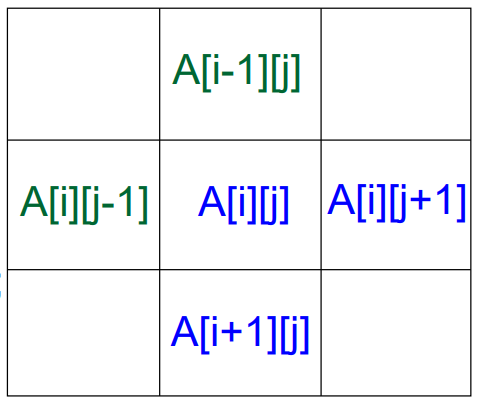
\includegraphics[width=0.6\textwidth]{images/grid.png}
    \caption{Grid points and their neighbours}
    \label{fig:grid}
\end{figure}

In each iteration, we sweep through all grid points, update the value at each point by averaging the values of its four (or more) immediate neighbours, and accumulate the absolute difference in the variable \texttt{diff}. We continue this process until \texttt{diff} falls below a given tolerance.

There are two classical iterative methods for this problem:

\begin{itemize}
    \item \textbf{Jacobi Method:} Uses neighbour values from the previous time step. All grid points are updated simultaneously using an auxiliary array to store the new values.
    
    \item \textbf{Gauss-Seidel Method:} Uses the most recently available values — i.e., when updating a grid point, the already-updated values from the current iteration (lower index values) are used whenever possible. This usually converges faster but is inherently more sequential.
\end{itemize}

To parallelize this computation, we need to decompose the grid into sub-regions that can be processed independently by different threads or processes. Each task will be responsible for a subset of grid points. However, care must be taken to handle boundary conditions and ensure proper synchronization or communication between tasks when accessing neighbouring values.

\begin{enumerate}
    \item One way is to consider each element in parallel. A parallel process or a parallel thread for each of the elements, i.e., a concurrent task for each element update. This would require a maximum concurrency of $n^2$ tasks (for $n \times n$ elements in the grid). Practically, this is not feasible as the number of tasks is very large, and the overhead of creating and managing the tasks is very high. This many parallel threads is not practically possible, as for larger values of $n$, the number of threads required will be $n^2$. Thus, many threads would have to be mapped to the same processors and would require a lot of context switching between threads and processes, which can affect the performance.

    \item Another way is to consider tasks for elements in the anti-diagonal. Note that values in a particular anti-diagonal depend on the values from the previous anti-diagonal but not among the elements within the same anti-diagonal. Now we consider a particular anti-diagonal—for some element in the anti-diagonal, using the Gauss-Seidel method, we require the values of the neighbours from the previous anti-diagonal at the latest time step and the value from the next anti-diagonal at the previous time step. This works out, since we are computing anti-diagonal by anti-diagonal, starting from the top-left corner and moving toward the bottom-right corner. Thus, the values of the neighbours are available from the previous anti-diagonal at the latest time step and the next anti-diagonal at the previous time step. Also, note that the values of the elements in the anti-diagonal are independent of each other and thus can be computed in parallel. This is as shown in the Figure~\ref{fig:anti-diag_examp}.
\begin{figure}[ht]
    \centering
    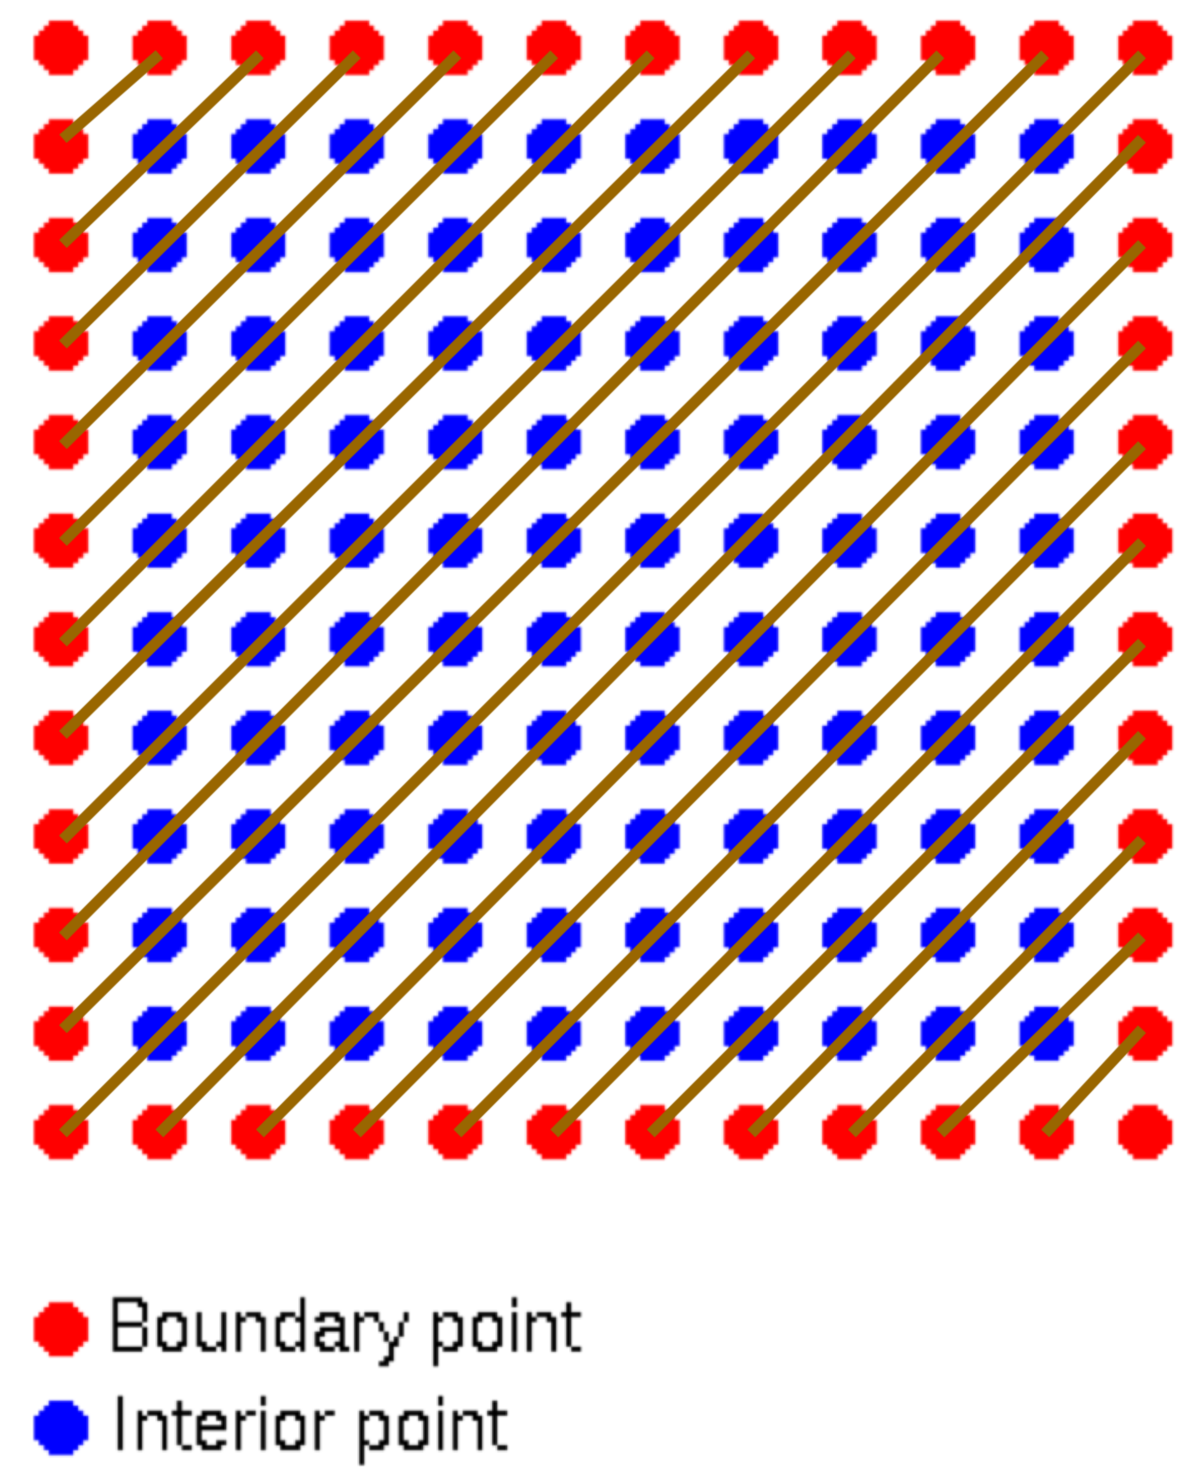
\includegraphics[width=0.5\linewidth]{images/Examp_anti2.png}
    \caption{Anti-diagonals}
    \label{fig:anti-diag_examp}
\end{figure}
    \vspace{5pt}
    Therefore, we can consider the tasks for the elements in the anti-diagonal and compute their values in parallel. This way, we can reduce the number of tasks to $2n - 1$ (for $n \times n$ elements in the grid). This is a better approach than the previous one, as the number of tasks is reduced and the tasks are independent of each other.

    \vspace{5pt}
    Note that for the diagonals at the ends, the number of elements will be smaller, and hence the parallelism will also be limited. This approach also incurs synchronization costs because the processes assigned to a particular diagonal cannot start executing until the earlier diagonals have finished executing. Thus, the parallelism is limited by the number of elements in the diagonal and the synchronization overhead.

    \item What we follow is block distribution of the data. Consider Figure~\ref{fig:block}, which shows the block distribution of the data.
    
    \begin{figure}[H]
        \centering
        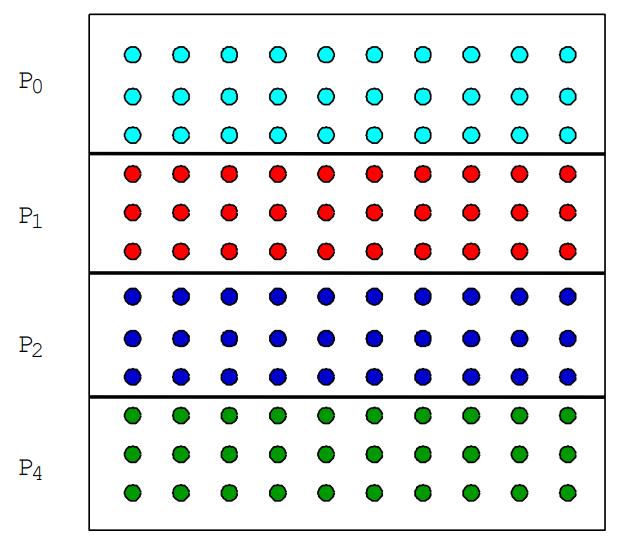
\includegraphics[width=0.6\textwidth]{images/block.png}
        \caption{Block Distribution}
        \label{fig:block}
    \end{figure}
    
    In this approach, we divide the 2D grid across the rows. The first set of rows is assigned to P0, the second set to P1, and so on. Each processor will be responsible for updating the values of the elements in the rows assigned to it.

    \vspace{5pt}
    For the orchestration step, we need to identify the synchronization and communication requirements. The goal is to ensure correctness while minimizing communication and synchronization calls. The implementation details depend on the underlying programming/model architecture—whether it is based on a shared memory model or a message-passing model.
\end{enumerate}


\subsubsection{Shared Address Space / Shared Memory Model}

Now we consider the Shared Address Space (SAS) version of the program, as shown in Listing~\ref{lst:shared}.

\begin{lstlisting}[style=cppstyle, caption={Shared Address Space Version}, captionpos=b, label={lst:shared}]
int n, nprocs; /* Matrix: (n+2) x (n+2) elements */
float **A, diff = 0;
LockDec(lock_diff);
BarrierDec(barrier1);

main()
begin
    read(n);           /* Read input parameter: matrix size */
    read(nprocs);      /* Read number of processors */
    
    A = malloc(a 2-D array of (n+2) x (n+2) floats);
    
    Create(nprocs - 1, Solve, A);  /* Spawn nprocs - 1 processes */
    
    initialize(A);     /* Initialize the matrix A */
    
    Solve(A);          /* Main process also solves */
    
    Wait_for_End(nprocs - 1);  /* Wait for other processes to finish */
end main
\end{lstlisting}

Note that we are using $(n+2)$ grid points to handle boundary conditions, but only \texttt{nprocs} processors. The array \texttt{A} is shared among all processes. The main process creates the other processes and then continues with solving. 

Let us now look at the pseudocode for the \texttt{Solve} function.

\begin{lstlisting}[style=cppstyle, caption={Solve Function}, captionpos=b, label={lst:solve}]
procedure Solve(A)  /* Solve the equation system */
float **A;
begin
    int i, j, pid, done = 0;
    float temp;

    mybegin = 1 + (n / nprocs) * pid;
    myend   = mybegin + (n / nprocs);

    while (!done) do  /* Outer loop over sweeps */
        diff = 0;  /* Initialize difference to 0 */

        Barrier(barrier1, nprocs);  /* Synchronize all processes */

        for (i = mybegin; i < myend; i++) do  /* Sweep over grid */
            for (j = 1; j <= n; j++) do
                temp = A[i][j];  /* Save old value */
                A[i][j] = 0.2 * (A[i][j] + A[i][j-1] + A[i-1][j] + A[i][j+1] + A[i+1][j]);  /* Compute average */
                diff += abs(A[i][j] - temp);
            end for
        end for

        if (diff / (n * n) < TOL) then
            done = 1;
    end while
end procedure
\end{lstlisting}



Now, this particular function is executed by all the processes. But depending on the process ID, different processes will handle different parts of the grid. This approach is called the \textbf{Single Program Multiple Data (SPMD)} model. The same program is executed by all processes, but each works on a different portion of the data.

The expressions 
\[
\texttt{mybegin} = 1 + \left(\frac{n}{\texttt{nprocs}}\right) \cdot \texttt{pid}, \quad \texttt{myend} = \texttt{mybegin} + \left(\frac{n}{\texttt{nprocs}}\right)
\]
determine the starting and ending rows of the grid that each process is responsible for. These are calculated using the process ID.

All the processes now enter the \texttt{while} loop. The matrix \texttt{A} and the variable \texttt{diff} are shared by all processes, making them global. At the beginning of each iteration, all processes synchronize using a \texttt{barrier}, as shown in the code.

Each process then executes the loop that updates a subset of the grid. Although every process runs the same code, they work on different rows depending on their \texttt{pid}. The elements in the grid are updated by computing an average, and the difference between the new and old values is added to \texttt{diff}.

Since \texttt{diff} is a shared variable, it gets updated by all the processes. At the end of the iteration, it is compared with a predefined tolerance to determine whether the loop should terminate.

This was just an overview of the program. To understand the benefits of parallel computing, it's important to appreciate synchronization primitives like the \texttt{barrier}.

A \texttt{barrier} is a synchronization point. When a process reaches a barrier, it waits there until all other processes have reached the same point. Only after that can any of the processes proceed. In the program above, this ensures that all processes finish their computation for one iteration before moving to the next. Without this, some processes might start the next iteration using stale values from neighboring processes that haven’t finished updating their part of the grid.

\begin{note}
    The matrix \texttt{A} is a global variable and is shared among all processes. During execution, each process updates its portion of the matrix. However, issues can arise at the boundaries between two adjacent processors.

    For example, if a process updates a boundary element before its neighboring process has finished updating its own value, inconsistent or stale values might be used. This can lead to incorrect results.

    One way to avoid this problem, especially in the Jacobi method, is to use a temporary array local to each process. This temporary array holds the updated values for the current iteration based on the global matrix values from the previous step. Once all processes have completed their local updates (ensured via a \texttt{barrier} call), the temporary arrays are copied back into the shared matrix \texttt{A}, and the next iteration begins.

    This ensures that all updates, especially at the boundaries, are synchronized. In our current discussion, we are ignoring this issue for simplicity and assuming that such synchronization is handled internally.
\end{note}
After solving the matrix \texttt{A}, the code in Listing~\ref{lst:shared} uses a \texttt{Wait\_for\_End} call. This makes the main process wait until all the other processes have finished. It can be implemented using an \textit{all-to-one} communication pattern, where each worker process sends a message to the main process to signal completion.

Note that the variable \texttt{diff} is a global (shared) variable. Since all processes read and write to it, it can lead to incorrect or garbage values due to race conditions. A race condition happens when multiple processes access and update a shared variable at the same time, leading to unpredictable results. This often arises because of context switching at the assembly level.

To solve this, we use \textbf{locks}. A lock is a mechanism that ensures only one process can access a shared resource at a time. When a process wants to update the shared variable, it first locks it, then accesses and modifies it, and finally unlocks it. This ensures exclusive access.

In computer science, a \textbf{lock} or \textbf{mutex} (short for mutual exclusion) is a synchronization primitive. It ensures that only one thread or process can acquire the lock at any given time. All other threads trying to acquire the lock are blocked until the lock is released. This ensures that shared resources are protected and accessed safely.

This concept is called \textbf{mutual exclusion} — processes exclude each other, allowing only one to enter the critical section (the part of the code accessing the shared variable). In our case, both \texttt{diff} and the matrix \texttt{A} are shared variables. So, care must also be taken when processes update boundary elements of the matrix. Those elements may be read and written by neighboring processes at the same time.

To avoid this, locks can also be used while updating matrix elements at the boundaries. However, another common and more efficient approach is to use a temporary matrix that is local to each process. Each process computes new values into its local matrix, based on the previous values in the global matrix. After all processes finish (synchronized using a \texttt{barrier}), they copy their local results into the global matrix. This approach is called \textbf{double buffering}.

Locks, while helpful, are expensive. If each grid point update needs to acquire a lock (especially for \texttt{diff}), it introduces a lot of waiting. Every process will have to wait for others to release the lock before updating \texttt{diff}. This adds overhead and reduces performance.

But here’s an observation: we only need \texttt{diff} at the end of each iteration — to check convergence. So, instead of updating the global \texttt{diff} every time, each process can maintain a \texttt{mydiff} variable locally. At the end of the iteration, all local \texttt{mydiff} values are added together to get the global \texttt{diff}. This is called a \textbf{reduction operation}. It significantly reduces locking overhead.

Previously, locks were required for each of the $\mathcal{O}(n^2)$ grid updates. Now, with local diffs and a single reduction step, we reduce the locking overhead to $\mathcal{O}(p)$, where $p$ is the number of processes — a huge improvement!

The updated \texttt{Solve} function with this idea is shown in Listing~\ref{lst:solve2}.

\begin{lstlisting}[style=cppstyle, caption={Updated Solve Function}, captionpos=b, label={lst:solve2}]
procedure Solve(A)  /* Solve the equation system */
float **A;
begin
    int i, j, pid, done = 0;
    float mydiff, temp;

    mybegin = 1 + (n / nprocs) * pid;
    myend   = mybegin + (n / nprocs);

    while (!done) do  /* Outer loop over sweeps */
        mydiff = diff = 0;  /* Initialize differences */

        Barrier(barrier1, nprocs);  /* Synchronize before sweep */

        for (i = mybegin; i < myend; i++) do  /* Grid sweep */
            for (j = 1; j <= n; j++) do
                temp = A[i][j];  /* Save old value */
                A[i][j] = 0.2 * (A[i][j] + A[i][j-1] + A[i-1][j] + A[i][j+1] + A[i+1][j]);
                mydiff += abs(A[i][j] - temp);
            end for
        end for

        lock(diff-lock);
            diff += mydiff;  /* Accumulate local diff to global diff */
        unlock(diff-lock);

        Barrier(barrier1, nprocs);  /* Synchronize before checking */

        if (diff / (n * n) < TOL) then
            done = 1;  /* Check convergence */
        
        Barrier(barrier1, nprocs);  /* Final barrier before next sweep */
    end while
end procedure
\end{lstlisting}
Note that in the updated pseudocode, a new local variable \texttt{mydiff} is introduced for each process. This variable is updated independently by each process during the iteration. At the end of the iteration, all local \texttt{mydiff} values are added together to get the global \texttt{diff} value, using the locking mechanism as shown in Listing~\ref{lst:solve2}.

The statements \texttt{lock(diff-lock)} and \texttt{unlock(diff-lock)} are used to acquire and release the lock on the shared \texttt{diff} variable. This reduces the contention for the lock, since it is needed only once per process per iteration, not for every grid point update.

A \texttt{barrier} call is placed after the accumulation step. This ensures that all processes have completed their computations and updated the global \texttt{diff} before any process checks the termination condition. Without this synchronization, some processes might check the condition before \texttt{diff} is fully updated, leading to incorrect results.

Another \texttt{barrier} is placed right after the termination condition check. This is important because if the condition is not met, one process might enter the next iteration and set \texttt{diff = 0} too early. Meanwhile, another process still evaluating the condition might see this incorrect zero value, which would be wrong. The second barrier ensures that all processes finish checking the correct value of \texttt{diff} before any of them proceed to the next iteration.

The assignment \texttt{done = 1} is done redundantly by all processes once convergence is reached. This is acceptable because the statement is identical to what appears in a sequential program.

This brings us to an important point. One of the advantages of shared memory programming is that the code structure remains close to the sequential version. Parallelism is introduced simply by adding constructs like \texttt{locks} and \texttt{barriers}. This makes shared memory programs easier to write and debug compared to message passing programs, where the entire structure is different and processes need to explicitly communicate using send and receive operations.


\subsubsection{Message Passing Version}

In the message passing model, we cannot assume that matrix \texttt{A} is a global shared array accessible to all processes. There is no concept of shared variables here. Each process must maintain its own local part of the matrix.

If a process needs values that were updated by another process, it must explicitly receive them through message passing. So, data has to be sent between processes.

We use \textit{domain decomposition} to divide the 2D domain among different processes. Each process follows the \textit{owner computes} rule, meaning the process responsible for a subdomain also computes values in that region.

Since there is no global data structure, each process maintains local data structures. This increases the need for communication. To handle this, we introduce something called \textbf{ghost rows}.

Ghost rows are explained in Figure~\ref{fig:ghost}.

\begin{figure}[H]
    \centering
    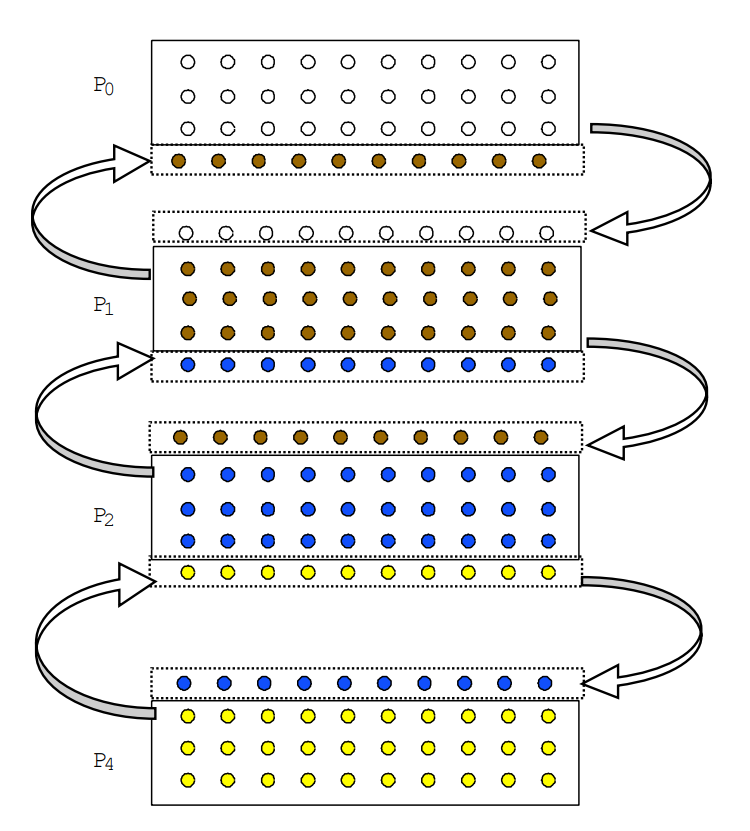
\includegraphics[width=0.6\textwidth]{images/ghost.png}
    \caption{Ghost Rows}
    \label{fig:ghost}
\end{figure}

In this figure~\ref{fig:ghost}, the 2D grid is divided among 4 processes, just like in the shared memory model. Each process is responsible for updating values in its assigned rows.

But unlike the shared memory model, each process now has its own local array to store these rows. In addition to this, each process has extra rows called \textbf{ghost rows}, as shown in the figure.

These ghost rows are used to store boundary values received from neighboring processes. For example:
\begin{itemize}
    \item Process 0 has a ghost row at the bottom to store the top boundary row from Process 1.
    \item Process 1 has a ghost row at the top for Process 0 and at the bottom for Process 2.
    \item And so on for the other processes.
\end{itemize}

Ghost rows are not updated by the process that holds them. Instead, they are updated by the neighboring processes that own the actual data. The purpose of ghost rows is to help compute local values at the boundaries using up-to-date data from neighbors.

Ghost rows are also called \textit{halo rows}, \textit{halo regions}, or \textit{ghost zone regions}.

Once each process receives the required ghost row data from its neighbors, it can simply perform local (sequential) computation using its local array.

Now consider the message passing version of the program shown in Listing~\ref{lst:mpi}.

\begin{lstlisting}[style=cppstyle,caption={Message Passing Version - Main Function},captionpos=b,label={lst:mpi}]
int n, nprocs; /* matrix: (n+2) x (n+2) elements */
float **myA;

main()
begin
    read(n);           /* read input parameter: matrix size */
    read(nprocs);      /* read number of processes */
    A = malloc(a 2-D array of (n+2) x (n+2) doubles);
    Create(nprocs-1, Solve, A);
    initialize(A);     /* initialize the matrix A somehow */
    Solve(A);
    Wait_for_End(nprocs-1);
end main
\end{lstlisting}


Now consider the \texttt{Solve} function for the message passing version, shown in Listing~\ref{lst:solve3}, which includes array allocation and ghost row communication.

\begin{lstlisting}[style=cppstyle,caption={MPI - Solve Function},captionpos=b,label={lst:solve3}]
procedure Solve(A) /* solve the equation system */
    float **A; /* A is a (n+2)-by-(n+2) array
begin
    int i, j, pid, done = 0;
    float mydiff, temp;
    myend = (n / nprocs);
    myA = malloc(array of (n / nprocs) x (n) floats);
    intialize(myA); /* Intialization myA locally*/
    
    while (!done) do /* outermost loop over sweeps */
        mydiff = 0; /* initialize local difference to 0 */

        if (pid != 0) then
            SEND(&myA[1,0], n * sizeof(float), (pid - 1), row);
        if (pid != nprocs - 1) then
            SEND(&myA[myend,0], n * sizeof(float), (pid + 1), row);
        if (pid != 0) then
            RECEIVE(&myA[0,0], n * sizeof(float), (pid - 1), row);
        if (pid != nprocs - 1) then
            RECEIVE(&myA[myend + 1,0], n * sizeof(float), (pid + 1), row);

        for (i = 1 to myend) do
            for (j = 1 to n) do
                temp = A[i,j]; /* save old value */
                A[i,j] = 0.2 * (A[i,j] + A[i,j-1] + A[i-1,j] + A[i,j+1] + A[i+1,j]); /* compute average */
                mydiff += abs(A[i,j] - temp);
            end for
        end for

        if (pid != 0) then
            SEND(mydiff, sizeof(float), 0, DIFF);
            RECEIVE(done, sizeof(int), 0, DONE);
        else
            for k = 1 to nprocs - 1 do
                RECEIVE(tempdiff, sizeof(float), k, DIFF);
                mydiff += tempdiff;
            end for
            if (mydiff / (n * n) < TOL) then done = 1;
            for k = 1 to nprocs - 1 do
                SEND(done, sizeof(int), k, DONE);
            end for
    end while
end procedure
\end{lstlisting}

In Listing~\ref{lst:solve3}, \texttt{myA} is the local array for each process. It stores the values of the grid elements corresponding to the domain allocated to the process—some subset of rows and all columns.

There are multiple ways to initialize these arrays: one option is to have each process read from a file; another is to let one process initialize the entire matrix and then distribute chunks to the others. For simplicity, we assume the processes are somehow able to initialize their local matrices.

Inside the \texttt{while} loop, each process maintains a local \texttt{mydiff} variable (note: no shared memory, so each process computes this separately).

At the start of each iteration, every process exchanges boundary rows with its neighboring processes:
\begin{itemize}
    \item If \texttt{pid} $\neq$ 0, the process sends its top row to \texttt{pid - 1}.
    \item If \texttt{pid} $\neq$ \texttt{nprocs - 1}, it sends its bottom row to \texttt{pid + 1}.
    \item Then, it receives the boundary rows from its neighbors and stores them in its \textbf{ghost rows}.
\end{itemize}

The ghost rows allow a process to compute its inner grid points using up-to-date boundary values received from neighbors. These ghost rows are only used for reading during the computation and are updated only via explicit communication (not by the owning process).

Once the ghost rows are updated, each process updates its portion of the grid just like in the sequential version. It also calculates its local difference \texttt{mydiff} during the update.

After computation:
\begin{itemize}
    \item Non-zero processes send their \texttt{mydiff} to process 0.
    \item Process 0 receives all \texttt{mydiff} values, aggregates them into a global \texttt{diff}, and checks the convergence condition.
    \item If convergence is met, it sends a \texttt{done} signal to all other processes.
    \item All processes exit the loop when \texttt{done = 1}.
\end{itemize}

This is how the message passing version of the program works using MPI-style pseudocode.


\subsection{Notes on Message Passing Version}

\begin{itemize}
    \item In the shared memory model, although there's no explicit communication, when one process writes to a variable and another reads it, this can still be seen as a form of communication. However, it is \textbf{receiver-initiated}, meaning the communication completes when the receiving process accesses the variable.

    \item In contrast, in the message passing model, communication is \textbf{sender-initiated}. A process must explicitly send data to another process using message-passing primitives like \texttt{SEND} and \texttt{RECEIVE}.

    \item Synchronization in the message passing model is \textbf{implicit}. Unlike in the shared memory model where synchronization is often done using explicit barriers, here it happens through communication operations. For instance, a \texttt{SEND} and \texttt{RECEIVE} pair naturally synchronizes two processes.

    \item This brings up a critical question: \textbf{can deadlocks occur in MPI communication?} Yes, they can. A deadlock may happen if all processes are stuck waiting for others to send data while none are sending anything.

    For example:
    \begin{itemize}
        \item All processes issue a \texttt{RECEIVE} before any \texttt{SEND}. Since no data is being sent, all processes block and wait indefinitely.
        \item Alternatively, all processes issue a blocking \texttt{SEND} that only completes when the data is received. But since no process is yet ready to receive, all \texttt{SEND}s block, leading again to a deadlock.
    \end{itemize}

    \item To avoid such situations, we can use \textbf{non-blocking communication} or design the program so that at least one process starts with a \texttt{SEND} and another with a \texttt{RECEIVE}.

    \item Such communication is called \textbf{synchronous communication}, where the \texttt{SEND} completes only after the matching \texttt{RECEIVE} starts. This ensures synchronization between processes.

    \item Communication is performed in entire rows at the beginning of each iteration — not point-by-point. This means an entire row is sent in one go instead of sending one grid point at a time, which is more efficient.

    \item Observe the communication pattern where each process sends its \texttt{mydiff} value to process 0, which aggregates all values to compute the global difference. This is an \textbf{All-to-One communication pattern}, known as a \textbf{reduction}.

    \item Reduction is a common pattern in parallel programming. Many parallel libraries provide built-in support for such operations. In this case, we add the local \texttt{mydiff} values using a reduction operation.

    \item After computing the global difference, the master process (process 0) broadcasts the \texttt{done} signal to all other processes. This is a \textbf{One-to-All communication}, also known as a \textbf{broadcast}.

    \item The original code using \texttt{SEND} and \texttt{RECEIVE} can be simplified using \texttt{REDUCE} and \texttt{BROADCAST} operations, as shown below:

\begin{lstlisting}[style=cppstyle]
/* Communicate local diff values and determine if done,
   using reduction and broadcast */
REDUCE(0, mydiff, sizeof(float), ADD);
if (pid == 0) then
    if (mydiff / (n * n) < TOL) then
        done = 1;
    endif
    BROADCAST(0, done, sizeof(int), DONE);
\end{lstlisting}

    \item The \texttt{REDUCE} operation collects the \texttt{mydiff} values from all processes at process 0 using an \texttt{ADD} operator to compute the global difference. Other operators like \texttt{MAX}, \texttt{MIN}, etc., can also be used depending on the need.

    \item After checking the termination condition, the master process uses \texttt{BROADCAST} to send the \texttt{done} signal to all other processes. This makes the communication more concise and efficient.
\end{itemize}


\subsection{Send and Receive Alternatives}

Recall that in the message-passing version, we used the \texttt{SEND} and \texttt{RECEIVE} operations to communicate data between processes. However, it may happen that the \texttt{SEND} operation causes the sending process to wait until the corresponding receiving process initiates its \texttt{RECEIVE} operation, and vice versa. This mutual waiting results in synchronous communication, where both sender and receiver are blocked until the message transfer is complete.

To avoid this blocking behavior, asynchronous communication can be used. Many MPI libraries support asynchronous \texttt{SEND} and \texttt{RECEIVE} operations, where a process does not need to wait for the corresponding operation on the other process to begin. In an asynchronous \texttt{SEND}, the sender proceeds without waiting for the receiver to initiate the \texttt{RECEIVE}. Similarly, in an asynchronous \texttt{RECEIVE}, the receiver does not block waiting for the sender to begin transmission.

Asynchronous operations can be further categorized into \textbf{blocking asynchronous} and \textbf{non-blocking asynchronous} variants. These will be discussed in detail in the MPI section.

\subsection{Summary}

\begin{itemize}
    \item \textbf{Shared Address Space (SAS)}: Shared and private data are explicitly separated. Communication occurs implicitly through shared memory access patterns. Synchronization is explicit, typically performed via atomic operations such as locks and barriers.
    
    \item \textbf{Message Passing}: There is no concept of shared memory; all data structures reside in local address spaces. Communication is explicit via \texttt{SEND} and \texttt{RECEIVE} operations. In the example discussed, synchronization is implicit—no explicit barrier is used—but explicit synchronization constructs also exist in message-passing models.
    
    \item While decomposition and assignment strategies were similar in both SAS and message-passing models, the key differences lie in orchestration and mapping. Table~\ref{tab:finsummary} summarizes the comparison:
\end{itemize}

\begin{table}[H]
    \centering
    \begin{tabular}{|p{0.5\textwidth}|c|c|}
        \hline
        & \textbf{Shared Address Space} & \textbf{Message Passing} \\
        \hline
        Explicit in global structure? & Yes & No \\
        Communication                 & Implicit & Explicit \\
        Synchronization               & Explicit & Implicit \\
        Explicit replication of border rows? & No & Yes \\
        \hline
    \end{tabular}
    \caption{Comparison between Shared Address Space and Message Passing Models}
    \label{tab:finsummary}
\end{table}
For more details on parallelization principles refer to sections 3.1 and 3.5 in~\cite{kumar1994introduction} and sections 2.2 and 2.3 in~\cite{culler1998parallel} for example.

\chapter{Shared Memory Parallelism - OpenMP}

Recall the term \textbf{processes} used in the context of shared memory address space models. In this setting, the term typically refers to \textbf{threads}. Threads are lightweight processes that share the same address space. Since multiple threads can access shared variables concurrently, synchronization mechanisms like barriers and locks are required to ensure data consistency and avoid race conditions.

The programmer must explicitly specify which variables are shared across threads and which are private to each thread. Because threads operate within the same address space, they can access common data structures and variables directly.

The most widely used programming interface for shared memory parallelism is OpenMP (Open Multi-Processing), a portable and scalable programming model. OpenMP provides a set of compiler directives, library routines, and environment variables to express parallelism at a high level in Fortran, C, and C++ programs.

So, what are compiler directives? These are special annotations or statements within the code that instruct the compiler to perform certain actions. For example, compilers support various optimization levels like \texttt{-O1}, \texttt{-O2}, etc. Through compiler directives, you can direct the compiler to optimize specific parts of the code selectively. In OpenMP, such directives are used to express shared-memory parallelism and are often referred to as \textbf{pragmas}.

One of the key advantages of OpenMP is that it makes parallel programming relatively simple. You can start with a serial program, then gradually insert OpenMP directives to indicate parallel regions, and finally compile and run the program with appropriate OpenMP flags to enable parallel execution.

The first version of OpenMP was released in 1997. As of now, the widely used version is OpenMP 6.0, released in 2024.


\section{Fork-Join Model}

OpenMP follows the \textbf{fork-join} execution model. The program begins with a single thread, known as the \textit{master thread}. When the program encounters a parallel construct, the master thread \textit{forks} a team of worker threads to execute the parallel region. Once the parallel region is completed, the worker threads \textit{join} back into the master thread, and execution resumes sequentially.

This behavior is illustrated in Figure~\ref{fig:forkjoin}.

\begin{figure}[H]
    \centering
    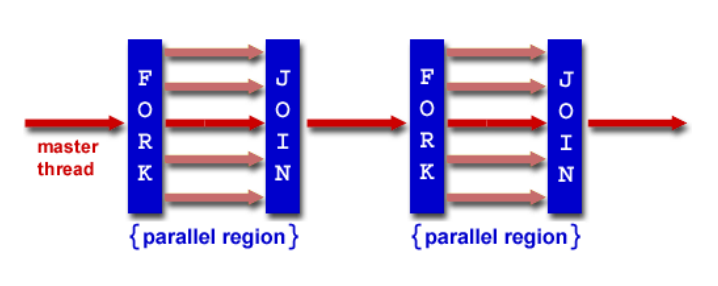
\includegraphics[width=0.6\textwidth]{images/forkjoin.png}
    \caption{Fork-Join Model}
    \label{fig:forkjoin}
\end{figure}

As seen in the figure, a single thread starts executing the program. Upon encountering a parallel region, a team of threads is spawned to execute that block in parallel. After completion, the threads synchronize and terminate, returning control to the master thread.

One of the major advantages of OpenMP is its support for \textbf{selective parallelism}—only specific regions of the code are parallelized based on need. This aligns well with \textbf{Amdahl's Law}, which highlights that only parts of a program are parallelizable while others must remain serial. OpenMP does not attempt to parallelize the entire program but instead allows the programmer to specify which regions benefit most from parallel execution.

OpenMP provides several key constructs to support parallel programming:
\begin{itemize}
    \item \textbf{Work-sharing constructs:} Specify how the work in a parallel region should be divided among the threads.
    \item \textbf{Synchronization constructs:} Ensure proper coordination and data consistency between threads.
    \item \textbf{Data environment constructs:} Define which variables are shared across threads and which are private to each thread.
    \item \textbf{Library routines and environment variables:} Provide utility functions and allow customization of the execution environment (e.g., setting the number of threads using environment variables before program execution).
\end{itemize}

A \textit{construct} in OpenMP refers to a compiler directive paired with the block of code (region) to which it applies.

OpenMP primarily supports \textbf{loop-level parallelism}, especially for \texttt{for}/\texttt{do} loops. If there are no loop-carried dependencies, iterations can be safely divided among threads. Each thread then executes a subset of the loop iterations. This offers \textbf{fine-grained parallelism}, giving the programmer detailed control over which specific regions of code are parallelized.

Additionally, OpenMP allows \textbf{dynamic parallelism}—the number of threads used in a parallel region can be varied based on computational load. Regions that benefit from greater parallelism can use more threads, while lighter regions may use fewer. This flexibility is useful for optimizing performance dynamically at runtime.

Alongside fine-grained parallelism, OpenMP also supports \textbf{coarse-grained parallelism}, where entirely different sections of the program are executed in parallel.

Modern versions of OpenMP include advanced features such as:
\begin{itemize}
    \item \textbf{Offloading to accelerators (e.g., GPUs):} Through target directives, specific regions of code can be executed on devices such as GPUs.
    \item \textbf{SIMD vectorization:} Enables automatic vectorized execution of operations across multiple data elements.
    \item \textbf{Task-core affinity:} Allows tasks to be pinned to specific cores, which can help reduce data movement and improve cache utilization.
\end{itemize}

These features make OpenMP not just a tool for simple parallelism, but a comprehensive framework suitable for modern multicore and heterogeneous architectures.


\section{Parallel Construct}

\texttt{\#pragma omp parallel} is the primary parallel construct in OpenMP.  
It is used to create a \textbf{team of threads}, where each thread executes the specified code block in parallel. The syntax is:

\begin{lstlisting}[style=cppstyle]
#pragma omp parallel
{
    /* parallel region */
}
\end{lstlisting}

This block of code is referred to as the \textbf{parallel region}. When the compiler encounters the \texttt{\#pragma omp parallel} directive, it forks a team of threads. Each thread in the team executes the code inside the braces.  
Before this directive is reached, the program executes sequentially on the \textbf{master thread}.

Thus, a \textbf{parallel construct} consists of the `parallel` directive and the corresponding code block that is executed concurrently by multiple threads.

\vspace{0.5em}
\noindent
\textbf{How many threads are created?}
This depends on how OpenMP is configured. There are several ways to control the number of threads:

\begin{itemize}
    \item Set the environment variable at runtime: \texttt{export OMP\_NUM\_THREADS=number}
    \item Use the function call: \texttt{omp\_set\_num\_threads(n);}
    \item Use the clause \texttt{num\_threads(n)} directly in the pragma directive.
\end{itemize}

\vspace{0.5em}
\noindent
OpenMP also provides various \textbf{clauses} to modify the behavior of the parallel region:

\begin{itemize}
    \item \texttt{if (condition)}: Executes the parallel region in parallel only if the condition evaluates to true; otherwise, it is executed serially by the master thread.
    \item \texttt{num\_threads(n)}: Specifies the exact number of threads to be used in the parallel region.
    \item \texttt{default(shared | none)}: Sets the default data-sharing attributes for variables—either shared or requiring explicit declaration.
    \item \texttt{private(list)}: Declares a list of variables that are private to each thread. Each thread gets its own uninitialized copy.
    \item \texttt{firstprivate(list)}: Like `private', but initializes each thread’s copy with the value of the variable outside the parallel region.
    \item \texttt{shared(list)}: Declares a list of variables to be shared across all threads.
    \item \texttt{copyin(list)}: For variables declared `threadprivate`, initializes the value of each thread’s copy with that of the master thread.
    \item \texttt{reduction(operator: list)}: Each thread gets a private copy of the listed variables, which are combined at the end of the parallel region using the specified operator (like `+', `*', `max', etc.).
    \item \texttt{proc\_bind(master | close | spread)}: Controls thread-to-core binding. `master' binds threads to the same core as the master thread; `close' places them on nearby cores; `spread' distributes them across cores.
\end{itemize}

\vspace{0.5em}
\noindent
Consider the following example, which prints the number of threads created inside a parallel region:

\begin{lstlisting}[style=cppstyle]
#include <omp.h>
#include <stdio.h>

int main()
{
    int nthreads;
    #pragma omp parallel
    {
        nthreads = omp_get_num_threads();
        printf("Number of threads = %d\n", nthreads);
    }
    return 0;
}
\end{lstlisting}

If, say, 4 threads were used, you’ll see the line "Number of threads = 4" printed 4 times—once by each thread.

\vspace{0.5em}
\noindent
Now consider a basic Hello World example in OpenMP:

\begin{lstlisting}[style=cppstyle]
#include <omp.h>
#include <stdio.h>

int main()
{
    int nthreads, tid;
    #pragma omp parallel private(nthreads, tid)
    {
        tid = omp_get_thread_num();
        printf(``Hello World from thread %d\n", tid);
    }
    return 0;
}
\end{lstlisting}

Here, each thread prints its own message. The `private' clause ensures that `tid' and `nthreads' are thread-local, preventing race conditions. Try running this code on your machine to see multiple "Hello World" messages printed in parallel.

\vspace{0.5em}
\noindent
OpenMP makes it straightforward to parallelize sequential programs incrementally. You can write the core logic sequentially and then wrap performance-critical sections with appropriate OpenMP constructs.

\section{Work Sharing Construct}
The work sharing construct in OpenMP is used to distribute work among multiple threads. Once multiple threads have been spawned using the \texttt{parallel} construct, the work sharing construct specifies how the workload should be divided among these threads.

There are three main types of work sharing constructs in OpenMP:
\begin{itemize}
    \item \textbf{loops} – used to distribute iterations of a loop among threads,
    \item \textbf{sections} – used to assign distinct code blocks to different threads,
    \item \textbf{single} – ensures that a particular block of code is executed by only one thread.
\end{itemize}


\subsection{for-loop}

The \texttt{for} construct is used to parallelize \texttt{for}-loops or \texttt{do}-loops in OpenMP using the syntax:
\begin{lstlisting}[style=cppstyle]
#pragma omp for [clause[, clause]...]
\end{lstlisting}

It is typically used inside a \texttt{parallel} region to distribute loop iterations among the threads. The following clauses can be used with the \texttt{for} construct:

\begin{itemize}
    \item \textbf{private(list)}: Specifies variables that are private to each thread.
    \item \textbf{firstprivate(list)}: Like \texttt{private}, but initializes each private copy with the value of the original variable.
    \item \textbf{lastprivate(list)}: The variable is made private, but its value from the last iteration is copied back after the loop.
    \item \textbf{linear(list)}: Specifies linear induction variables with a fixed step size.
    \item \textbf{reduction(operator:list)}: Performs a reduction on the specified variables using the given operator across threads.
    \item \textbf{schedule([modifier:]kind[,chunk])}: Controls how iterations are divided among threads.
    \item \textbf{collapse(n)}: Useful for nested loops—collapses \texttt{n} nested loops into a single loop with a larger iteration space for parallelization.
    \item \textbf{ordered(n)}: Enforces ordered execution for sections of code marked with \texttt{ordered}.
    \item \textbf{nowait}: Prevents implicit barrier synchronization at the end of the loop. Threads need not wait for others.
\end{itemize}

The \texttt{for} construct is one of the most commonly used and important constructs in OpenMP. It assumes that loop iterations are independent of one another, i.e., there are no dependencies between iterations. If such dependencies exist—e.g., an iteration relies on the result of a previous iteration—then the \texttt{for} construct should not be used.

\paragraph{Schedule Clause:}  
The \texttt{schedule} clause determines how loop iterations are assigned to threads. OpenMP supports several scheduling policies:

\begin{enumerate}
    \item \textbf{schedule(static, chunk)}: Divides the iteration space into equal-sized chunks (of size \texttt{chunk}) and assigns them to threads in round-robin fashion.
    
    For example, consider a loop with 20 iterations and a chunk size of 2. Ten chunks are created, and with four threads, chunks are assigned as:
    \[
    \text{Thread 0: } \text{chunk 0, 4, 8}; \quad \text{Thread 1: } \text{chunk 1, 5, 9}; \text{...}
    \]

    \item \textbf{schedule(dynamic, chunk)}: Also splits the loop into chunks, but assigns them to threads dynamically at runtime. Threads that finish early can grab the next available chunk.
    
    \item \textbf{schedule(runtime)}: Defers scheduling strategy selection to runtime based on environment variables or OpenMP runtime configuration.
\end{enumerate}

\paragraph{Example:} Consider the following program that performs element-wise addition of two arrays:

\begin{lstlisting}[style=cppstyle, caption={Addition of Two Arrays Using \texttt{for} Construct}, label={lst:for-example}]
#include <omp.h>
#define CHUNKSIZE 100
#define N 1000

int main(){
    int i, chunk;
    float a[N], b[N], c[N];

    // Initialization
    for (i = 0; i < N; i++)
        a[i] = b[i] = i * 1.0;

    chunk = CHUNKSIZE;

    #pragma omp parallel shared(a, b, c, chunk) private(i)
    {
        #pragma omp for schedule(dynamic, chunk) nowait
        for (i = 0; i < N; i++) {
            c[i] = a[i] + b[i];
        }
    }

    return 0;
}
\end{lstlisting}

In this example, we are adding arrays \texttt{a} and \texttt{b} to produce \texttt{c}. Since each element-wise addition is independent, this is a good candidate for parallelization.

We use \texttt{\#pragma omp parallel} to create threads. The variables \texttt{a}, \texttt{b}, \texttt{c}, and \texttt{chunk} are marked as \texttt{shared} because they need to be accessed by all threads, while \texttt{i} is marked as \texttt{private} since each thread should have its own loop counter to avoid conflicts.

The inner \texttt{for} loop is parallelized using the \texttt{for} construct with \texttt{schedule(dynamic, chunk)} to allow dynamic load balancing. The \texttt{nowait} clause prevents threads from waiting for others once their iterations are complete.

Note that the two pragmas can be combined into a single directive as follows:

\begin{lstlisting}[style=cppstyle]
#pragma omp parallel for shared(a, b, c, chunk) private(i) schedule(dynamic, chunk) nowait
\end{lstlisting}


\subsection{Coarse-Level Parallelism — Sections and Tasks}

In addition to fine-level parallelism (as seen in the \texttt{for} loop example), OpenMP supports \textbf{coarse-level parallelism}. 

While fine-level parallelism typically deals with distributing iterations of a loop among multiple threads, coarse-level parallelism involves executing \textbf{independent blocks of code}—like separate functions or computational phases—in parallel.

\paragraph{Sections Construct:}
If we want to execute two or more independent code blocks (e.g., different functions) concurrently, OpenMP provides the \texttt{sections} construct. This allows different threads to execute different code blocks in parallel, rather than all threads executing the same block of code as in \texttt{for} loops.

Consider the example shown in listing \ref{lst:sections}:

\begin{lstlisting}[style=cppstyle, caption={Sections Construct}, captionpos=b, label={lst:sections}]
#pragma omp parallel sections [clauses]
{
    #pragma omp section
    {
        // structure block i (e.g., function1());
    }

    #pragma omp section
    {
        // structure block j (e.g., function2());
    }
    ...
}
\end{lstlisting}

In this example, each \texttt{\#pragma omp section} defines a code block (or task) that can be executed by a separate thread. The enclosing \texttt{parallel sections} directive spawns a team of threads, and each section is assigned to one thread for execution. This is useful when you have multiple, independent tasks that can be run concurrently.

\paragraph{Tasks Construct:}

OpenMP also supports dynamic task creation using the \texttt{task} construct. This is useful in scenarios such as recursive algorithms, adaptive simulations, or when the number and structure of tasks are not known in advance.

Inside a parallel region, individual threads can create tasks using the \texttt{task} directive. These tasks are then dynamically assigned to available threads by the OpenMP runtime system. This enables load balancing and fine control over task execution.

Here’s a simplified example of the \texttt{task} construct, shown in listing \ref{lst:tasks}:

\begin{lstlisting}[style=cppstyle, caption={Tasks Construct}, captionpos=b, label={lst:tasks}]
#pragma omp parallel
{
    #pragma omp single
    {
        #pragma omp task
        {
            // Task 1 code
        }

        #pragma omp task depend(in: x)
        {
            // Task 2 depends on variable x from Task 1
        }
    }
}
\end{lstlisting}

In the above code:

- \texttt{\#pragma omp single} ensures only one thread in the team creates tasks (preventing all threads from redundantly spawning the same tasks).
- \texttt{\#pragma omp task} defines a task to be executed by any thread.
- The \texttt{depend} clause allows specifying task dependencies.

\paragraph{Task Dependencies and Task Graphs:}

OpenMP's \texttt{depend} clause enables you to define data dependencies between tasks. For instance, if Task 2 depends on a variable modified by Task 1, you can ensure that Task 2 will only execute once Task 1 has completed. This forms a \textbf{task dependency graph}, where:
\begin{itemize}
\item \textbf{Nodes} represent tasks.
\item \textbf{Edges} represent dependencies.
\end{itemize}
The OpenMP runtime builds and schedules this graph automatically, respecting the constraints provided. This powerful feature enables writing highly dynamic and dependency-aware parallel programs.

Thus, tasks enable \textbf{dynamic coarse-level parallelism} where the number and structure of tasks can evolve during runtime, while also maintaining control over execution order through explicit dependencies.


\section{Synchronization Directives}

Once the work is distributed among threads, there is always a possibility that multiple threads may access and update common variables simultaneously. This can lead to race conditions and inconsistent results. Therefore, we need to synchronize threads and protect shared data using appropriate locking or ordering mechanisms.

OpenMP provides several synchronization directives for this purpose. Note that all these constructs must be enclosed within a parallel region (created by a parallel construct):

\begin{itemize}
    \item \texttt{\#pragma omp master}: The block of code following this directive is executed only by the master thread. This is useful, for example, when only one thread (typically the master) should perform tasks like printing to the console to avoid cluttered output.

    \item \texttt{\#pragma omp critical}: Ensures that the enclosed block is executed by only one thread at a time. This is useful for updating shared variables, where concurrent access by multiple threads could lead to inconsistent or garbage values.

    \item \texttt{\#pragma omp barrier}: Forces all threads in the team to wait at this point until every thread has reached it. Useful for synchronization at intermediate stages of the parallel region.

    \item \texttt{\#pragma omp atomic}: Ensures that the specific memory operation (such as a simple update to a variable) following this directive is executed atomically—only one thread performs the update at a time, but with lower overhead than a full critical section.

    \item \texttt{\#pragma omp ordered}: Specifies that the block of code should be executed in the order of thread IDs. This is helpful when we need ordered output—for example, when printing parts of an array sequentially from multiple threads.

    \item \texttt{\#pragma omp flush}: Ensures memory consistency between threads by forcing a thread’s private view of memory to be synchronized with shared memory. This is particularly useful when a thread updates a shared variable, and other threads must see the updated value immediately.

    Consider the following example using the \texttt{flush} directive, shown in listing \ref{lst:flush}.

\begin{lstlisting}[style=cppstyle, caption={Flush Directive}, captionpos=b, label={lst:flush}]
int sync[NUMBER_OF_THREADS];
float work[NUMBER_OF_THREADS];

#pragma omp parallel private(iam, neighbor) shared(work, sync)
{
    iam = omp_get_thread_num();
    sync[iam] = 0;
    #pragma omp barrier

    // Perform computation and write result to shared array
    work[iam] = compute(iam);

    // Announce completion of work
    #pragma omp flush(work)      // Ensure work is visible to other threads
    sync[iam] = 1;
    #pragma omp flush(sync)      // Ensure sync is updated in shared memory

    // Wait for neighbor to complete its work
    neighbor = (iam > 0 ? iam : omp_get_num_threads()) - 1;
    while (sync[neighbor] == 0) {
        #pragma omp flush(sync)
    }

    // Read neighbor's result
    ... = work[neighbor];
}
\end{lstlisting}

In this example, each thread computes its result and writes it to the shared \texttt{work} array. Neighboring threads need access to this data, so we use the \texttt{flush} directive to ensure memory visibility.

- The first \texttt{flush(work)} guarantees that the result written by a thread is visible to other threads before it signals completion.
- The update \texttt{sync[iam] = 1} is used to notify others that the computation is complete.
- The second \texttt{flush(sync)} ensures that this flag is visible to all threads.
- The neighbor thread checks \texttt{sync[neighbor]} in a loop and repeatedly flushes it until the update is visible.
- Once visible, it safely accesses \texttt{work[neighbor]}.

This pattern provides a consistent memory view and safe inter-thread communication. The \texttt{flush} directive is essential when shared variables are updated by one thread and read by others soon after.

\end{itemize}


\section{Data Scope Attribute Clauses}

OpenMP provides several clauses to control the scope and visibility of variables in parallel regions. These are known as \textit{data scope attribute clauses}.

\begin{enumerate}
    \item \textbf{private(list):} Each thread gets its own uninitialized copy of the variable(s) in the list. These variables are not shared and are re-created per thread.

    \item \textbf{firstprivate(list):} Similar to \texttt{private}, but each thread's copy is initialized with the value the variable had in the master thread before entering the parallel region.

    \item \textbf{lastprivate(list):} Like \texttt{private}, but the value from the last iteration (or the last thread to execute the region) is copied back to the original variable after the region ends.

    \item \textbf{shared(list):} All threads share the same memory location for the listed variables. Any update by one thread is visible to all others.

    \item \textbf{default(shared/private/none):} Sets the default sharing behavior for all variables not explicitly listed in other clauses. \texttt{default(none)} forces all variables to be explicitly scoped.

    \item \textbf{reduction(operator:list):} A private copy is created for each thread. After the parallel region, the copies are combined using the specified operator and assigned to the original variable.

    \item \textbf{copyin(list):} Used with \texttt{threadprivate} variables. Copies the master thread's value of the variable(s) to all threads at the beginning of a parallel region.

    \item \textbf{copyprivate(list):} Used in a \texttt{single} construct to copy the value of a private variable from one thread to all others once the construct ends.
\end{enumerate}

\vspace{10pt}

Declaring large multidimensional arrays as \texttt{private} leads to significant overhead because each thread allocates a copy. Using \texttt{firstprivate} adds further overhead due to per-thread initialization.

\subsection{threadprivate}

The \texttt{threadprivate} directive makes a global variable behave like a private variable — each thread has its own copy — but with values preserved across multiple parallel regions.

\begin{lstlisting}[style=cppstyle, caption={threadprivate Directive}, captionpos=b, label={lst:threadprivate}]
#include <omp.h>
int alpha[10], beta[10], i;
#pragma omp threadprivate(alpha)

main() {
    omp_set_dynamic(0); // Disable dynamic threads

    // First parallel region
    #pragma omp parallel private(i, beta)
    for (i = 0; i < 10; i++)
        alpha[i] = beta[i] = i;

    // Second parallel region
    #pragma omp parallel
    printf("alpha[3] = %d and beta[3] = %d\n", alpha[3], beta[3]);
}
\end{lstlisting}

\texttt{alpha} retains its value in the second region due to \texttt{threadprivate}. \texttt{beta}, being merely \texttt{private}, does not preserve its value across regions.

To ensure thread consistency, the number of threads must be the same across regions. Hence, \texttt{omp\_set\_dynamic(0)} is used to disable dynamic thread allocation.

\subsection{default-example}

This example demonstrates the use of \texttt{default(none)}, along with \texttt{private}, \texttt{shared}, and \texttt{threadprivate} clauses.

\begin{lstlisting}[style=cppstyle, caption={default-Example}, captionpos=b, label={lst:default}]
int x, y, z[1000];
#pragma omp threadprivate(x)

void fun(int a) {
    const int c = 1;
    int i = 0;

    #pragma omp parallel default(none) private(a) shared(z)
    {
        int j = omp_get_num_thread(); // Thread-local variable
        a = z[j];     // OK: 'a' is private, 'z' is shared
        x = c;        // OK: 'x' is threadprivate, 'c' is const
        z[i] = y;     // ERROR: 'i' and 'y' not in any clause
    }
}
\end{lstlisting}

\begin{itemize}
    \item \texttt{x} is \texttt{threadprivate}, so assignment \texttt{x = c} is legal.
    \item \texttt{a} is declared \texttt{private}, and \texttt{z} is shared, so \texttt{a = z[j]} is valid.
    \item \texttt{z[i] = y} fails because \texttt{i} and \texttt{y} are not listed in any clause and \texttt{default(none)} prevents implicit sharing.
\end{itemize}


\section{Library Routines (API)}

In addition to compiler directives and data-sharing clauses, OpenMP provides a powerful set of runtime library routines that offer functionality such as:

\begin{itemize}
    \item Querying the OpenMP execution environment (e.g., number of threads, thread IDs).
    \item Managing locks and mutual exclusion.
    \item Configuring execution policies (e.g., dynamic threads, nested parallelism).
\end{itemize}

These functions are defined in the \texttt{omp.h} header file and can be categorized as follows:

\subsection{1. Query Functions}
\begin{itemize}
    \item \texttt{omp\_get\_num\_threads()}: Returns the number of threads in the current team.
    \item \texttt{omp\_get\_max\_threads()}: Returns the maximum number of threads available.
    \item \texttt{omp\_get\_thread\_num()}: Returns the thread ID of the calling thread (from 0 to \texttt{n-1}).
    \item \texttt{omp\_get\_num\_procs()}: Returns the number of processors available.
    \item \texttt{omp\_in\_parallel()}: Returns true (non-zero) if called inside a parallel region.
\end{itemize}

\subsection{2. Execution Environment Control}
\begin{itemize}
    \item \texttt{omp\_set\_num\_threads(int num)}: Requests that \texttt{num} threads be used in subsequent parallel regions.
    \item \texttt{omp\_set\_dynamic(int flag)}: Enables/disables dynamic adjustment of the number of threads.
    \item \texttt{omp\_get\_dynamic()}: Returns whether dynamic threads are enabled.
    \item \texttt{omp\_set\_nested(int flag)}: Enables/disables nested parallel regions.
    \item \texttt{omp\_get\_nested()}: Returns whether nested parallelism is enabled.
\end{itemize}

\subsection{3. Locking Routines}
OpenMP provides two types of locks: regular locks and nested locks. Nested locks allow reentrant locking by the same thread.

\begin{itemize}
    \item \texttt{omp\_lock\_t lock;} \quad \texttt{omp\_nest\_lock\_t nlock;} — Lock types.
    \item \texttt{omp\_init\_lock(\&lock)} / \texttt{omp\_init\_nest\_lock(\&nlock)} — Initialize a lock.
    \item \texttt{omp\_destroy\_lock(\&lock)} / \texttt{omp\_destroy\_nest\_lock(\&nlock)} — Destroy a lock.
    \item \texttt{omp\_set\_lock(\&lock)} / \texttt{omp\_set\_nest\_lock(\&nlock)} — Acquire a lock.
    \item \texttt{omp\_unset\_lock(\&lock)} / \texttt{omp\_unset\_nest\_lock(\&nlock)} — Release a lock.
    \item \texttt{omp\_test\_lock(\&lock)} / \texttt{omp\_test\_nest\_lock(\&nlock)} — Attempt to acquire lock without blocking.
\end{itemize}

\subsection{4. Timing Functions}
Used for profiling and benchmarking.

\begin{itemize}
    \item \texttt{omp\_get\_wtime()}: Returns elapsed wall-clock time (in seconds).
    \item \texttt{omp\_get\_wtick()}: Returns resolution (tick) of the timer used by \texttt{omp\_get\_wtime()}.
\end{itemize}

\vspace{0.5em}
These APIs give fine-grained control over OpenMP's runtime behavior, enabling programmers to build high-performance, scalable, and thread-safe applications.


\section{Locks}

OpenMP supports both \textbf{simple locks} and \textbf{nestable locks}. 

\paragraph{Simple Locks:} A simple lock can only be acquired once by a thread. If a thread that already holds a simple lock attempts to acquire it again (i.e., calls \texttt{omp\_set\_lock} twice in a row), a deadlock will occur. This is because only the thread that currently holds the lock can release it, and if it waits on itself, it will wait forever. Therefore, simple locks must never be nested.

\paragraph{Nestable Locks:} In contrast, \textbf{nestable locks} allow a thread to acquire the same lock multiple times without causing a deadlock. Internally, OpenMP maintains a counter for the number of times the lock has been acquired by the same thread. The lock is only released when the number of \texttt{omp\_unset\_nest\_lock()} calls matches the number of \texttt{omp\_set\_nest\_lock()} calls. 

Nestable locks are especially useful in complex software such as numerical libraries where multiple paths in a program may enter critical functions that need mutual exclusion.

\vspace{1em}
\noindent
The key distinctions between the two types of locks are:
\begin{itemize}
    \item \textbf{Simple lock:} Cannot be acquired recursively. Available only if currently unlocked.
    \item \textbf{Nestable lock:} Can be acquired recursively by the same thread. Considered available if either unlocked or already owned by the calling thread.
\end{itemize}

\subsubsection*{Example: Nested Lock Usage}

Consider the following example illustrating the need for nested locks, shown in Listing~\ref{lst:nested}:

\begin{lstlisting}[style=cppstyle, caption={Nested lock — Function design},captionpos=b,label={lst:nested}]
#include <omp.h>

typedef struct {
    int a, b;
    omp_nest_lock_t lck;
} pair;

void incr_a(pair *p, int a)
{
    // Called only from incr_pair, no need to lock
    p->a += a;
}

void incr_b(pair *p, int b)
{
    // Called both from incr_pair and elsewhere,
    // hence must be protected with a nested lock

    omp_set_nest_lock(&p->lck);
    p->b += b;
    omp_unset_nest_lock(&p->lck);
}
\end{lstlisting}

In this example:
\begin{itemize}
    \item The structure \texttt{pair} holds two integers \texttt{a}, \texttt{b} and a nested lock \texttt{lck}.
    \item \texttt{incr\_a()} is called only from \texttt{incr\_pair()}, hence no locking is required.
    \item \texttt{incr\_b()} is invoked from both \texttt{incr\_pair()} and elsewhere concurrently, so we must protect it with a nested lock.
\end{itemize}

\subsubsection*{Example Continued: Parallel Region with Nested Locks}

Now we illustrate a complete example using OpenMP sections to call both \texttt{incr\_pair()} and \texttt{incr\_b()} in parallel. This is shown in Listing~\ref{lst:nested2}:

\begin{lstlisting}[style=cppstyle, caption={Nested lock — Parallel sections},captionpos=b,label={lst:nested2}]
void incr_pair(pair *p, int a, int b)
{
    omp_set_nest_lock(&p->lck);
    incr_a(p, a);
    incr_b(p, b);
    omp_unset_nest_lock(&p->lck);
}

void f(pair *p)
{
    extern int work1(), work2(), work3();

    #pragma omp parallel sections
    {
        #pragma omp section
        incr_pair(p, work1(), work2());

        #pragma omp section
        incr_b(p, work3());
    }
}
\end{lstlisting}

\noindent
Explanation:
\begin{itemize}
    \item \texttt{f()} defines a parallel region with two sections.
    \item One thread executes \texttt{incr\_pair()} which internally calls both \texttt{incr\_a()} and \texttt{incr\_b()}.
    \item Another thread directly calls \texttt{incr\_b()}.
    \item Since \texttt{incr\_b()} may be accessed concurrently, and can be nested inside \texttt{incr\_pair()}, a \textbf{nested lock} is necessary to avoid race conditions and deadlocks.
\end{itemize}

This example clearly demonstrates how nested locks are essential when a function may be both independently and dependently called, and shared data must be safely modified under concurrent access patterns.



\subsection{Example 1: Jacobi Solver}

This example implements the Jacobi iterative method for solving discretized grid-based problems (such as Laplace's equation), except here we are parallelizing across \emph{iterations} (i.e., grid points) instead of just rows.

Consider the following code, shown in Listing~\ref{lst:jacobi}:

\begin{lstlisting}[style=cppstyle, caption={Jacobi solver using OpenMP}, captionpos=b, label={lst:jacobi}]
#include <omp.h>
#include <stdlib.h>

int main(int argc, char** argv){
    ...
    int rows, cols;
    int* grid;
    int chunk_size, threads = 16;
    int i, j;

    // Allocate and initialize the grid
    grid = malloc(sizeof(int) * rows * cols);
    for (i = 0; i < rows; i++) {
        for (j = 0; j < cols; j++) {
            grid[i * cols + j] = ...; // Some initialization
        }
    }

    chunk_size = rows / threads;

    #pragma omp parallel for num_threads(16) 
        private(i, j) shared(rows, cols, grid) 
        schedule(static, chunk_size) collapse(2)
    for (i = 1; i < rows - 1; i++) {
        for (j = 1; j < cols - 1; j++) {
            grid[i * cols + j] = 0.25 * (
                grid[i * cols + (j - 1)] + grid[i * cols + (j + 1)] +
                grid[(i - 1) * cols + j] + grid[(i + 1) * cols + j]
            );
        }
    }
    ...
    return 0;
}
\end{lstlisting}

As seen in the code, we initialize a 2D grid stored in a flattened 1D array. The Jacobi update computes each internal point as the average of its four neighbors (left, right, top, and bottom).

To parallelize the computation using OpenMP:
\begin{itemize}
    \item We define \texttt{chunk\_size} as \texttt{rows / threads}, which controls the number of iterations (in terms of row blocks) assigned per thread.
    \item The \texttt{\#pragma omp parallel for} directive initiates parallel execution of the nested loops using 16 threads.
    \item Variables \texttt{i} and \texttt{j} are declared as \texttt{private} to ensure each thread gets its own copy.
    \item \texttt{rows}, \texttt{cols}, and the pointer to \texttt{grid} are declared \texttt{shared} since all threads work on the same data array.
    \item \texttt{schedule(static, chunk\_size)} ensures iterations are distributed statically in contiguous blocks to the threads, which is efficient for load-balanced problems.
    \item The \texttt{collapse(2)} clause combines both loops into a single iteration space of size \texttt{(rows - 2) * (cols - 2)}. This allows better load balancing by distributing the total work across threads, rather than just distributing outer loop iterations.
\end{itemize}

Had we not used \texttt{collapse(2)}, only the outer loop (over \texttt{i}) would have been parallelized. In such a case, each thread would be responsible for all iterations of the inner loop (\texttt{j}), potentially causing load imbalance and underutilization of cores, especially for small \texttt{rows}.



\subsection{Breadth First Search (BFS) Algorithm}

The Breadth First Search (BFS) algorithm explores a graph level by level. Starting from a given source vertex at level $0$, BFS first visits all its immediate neighbors (level $1$), then the neighbors of those neighbors (level $2$), and so on, until all reachable vertices are visited. This traversal pattern makes BFS naturally parallelizable at each level of the graph.

We now present two parallel implementations of BFS: one using \textbf{nested parallelism}, and the other using \textbf{task-based parallelism}.

\subsubsection{Version 1: Nested Parallelism}

The following code snippet (Listing~\ref{lst:bfsv1}) illustrates a BFS implementation using nested \texttt{parallel for} constructs.

\begin{lstlisting}[style=cppstyle, caption={Parallel BFS using nested parallelism}, captionpos=b, label={lst:bfsv1}]
...
level[0] = {s};
curLevel = 0;
dist[s] = 0;
for (v != s) dist[v] = -1;

while (level[curLevel] != NULL) {
    #pragma omp parallel for ...
    for (i = 0; i < length(level[curLevel]); i++) {
        v = level[curLevel][i];
        neigh = neighbors(v);

        #pragma omp parallel for ...
        for (j = 0; j < length(neigh); j++) {
            w = neigh[j];
            if (dist[w] == -1) {
                level[curLevel + 1] = union(level[curLevel + 1], w);
                dist[w] = dist[v] + 1;
            }
        }
    }
}
\end{lstlisting}

In this approach:
\begin{itemize}
    \item We initialize the BFS by placing the source vertex $s$ at level $0$ and marking all other vertices as unvisited (distance = $-1$).
    \item For each level, we use the outer \texttt{\#pragma omp parallel for} to parallelize across the current level's vertices.
    \item For each vertex $v$ at this level, we obtain its neighbors and use an inner \texttt{parallel for} to visit all neighbors in parallel.
    \item If a neighbor $w$ has not yet been visited (i.e., \texttt{dist[w] == -1}), we add it to the next level and update its distance.
\end{itemize}

This is an example of \textbf{nested parallelism}: for each thread processing a vertex in the outer loop, additional threads are spawned to process its neighbors.

\subsubsection{Version 2: Task-Based Parallelism}

The next version (Listing~\ref{lst:bfsv2}) uses OpenMP tasks to dynamically create units of work for visiting each neighbor.

\begin{lstlisting}[style=cppstyle, caption={Parallel BFS using OpenMP tasks}, captionpos=b, label={lst:bfsv2}]
...
level[0] = {s};
curLevel = 0;
dist[s] = 0;
for (v != s) dist[v] = -1;

while (level[curLevel] != NULL) {
    #pragma omp parallel
    {
        #pragma omp single
        for (v in level[curLevel]) {
            for (w in neighbors(v)) {
                #pragma omp task
                {
                    if (dist[w] == -1) {
                        level[curLevel + 1] = union(level[curLevel + 1], w);
                        dist[w] = dist[v] + 1;
                    }
                }
            }
        }
    }
}
\end{lstlisting}

In this version:
\begin{itemize}
    \item We begin with a \texttt{parallel} region and enclose the main loop with a \texttt{single} directive to avoid redundant loop execution.
    \item For each neighbor of a vertex, we dynamically spawn an \texttt{omp task} to evaluate whether that neighbor should be added to the next level.
    \item Tasks are scheduled dynamically by OpenMP’s runtime system and assigned to available threads, improving efficiency in irregular graphs.
\end{itemize}

This method is more \textbf{adaptive} and \textbf{scalable}, especially in graphs with high variation in vertex degrees, since tasks can be scheduled independently and load-balanced across cores at runtime.

For further details on OpenMP, I would suggest the reader to refer to~\cite{llnlOpenMP} for tutorials on OpenMP or YouTube Lectures by Intel~\cite{openmpYoutube} and official website of OpenMP~\cite{openmpOfficial} to get a more indepth and broader understanding of OpenMP concepts. The ppt referred in the lectures can be found in the YouTube description and serves as an excellent guide for understanding the lectures as well as OpenMP overall in general.

\chapter{Message Passing Interface (MPI)}

MPI is a standardized and portable message-passing system designed to enable distributed-memory parallelism. Unlike shared memory paradigms such as OpenMP—where parallelism is achieved implicitly through directives—MPI requires explicit communication and synchronization between processes. This results in higher programming complexity, as each process must execute a specific program that communicates with others explicitly. For a gentler introduction refer to the last four YouTube lectures by Prof. Mathew Jacob on High performance Computing (HPC)~\cite{nptel-hpc-intro}.

Despite its complexity, MPI remains the dominant model for large-scale high-performance computing (HPC). This is because, although modern compute nodes may contain many cores and support shared-memory programming within a node, large-scale scientific and engineering problems often exceed the capacity of a single node. In such cases, multiple nodes must collaborate. Since nodes cannot directly access each other’s memory, communication between them must occur via message passing. This is where MPI becomes indispensable.

MPI is especially well-suited for:
\begin{itemize}
    \item Cluster computing, where each node has its own local memory.
    \item Large-scale simulations in scientific computing.
    \item Explicit control over data distribution and parallel execution.
\end{itemize}

In this chapter, we will explore:
\begin{itemize}
    \item The basic execution model of MPI.
    \item Communication primitives such as point-to-point and collective communication.
    \item Process topologies, communicators, and derived data types.
    \item Practical code examples to reinforce concepts.
\end{itemize}


\section{MPI Introduction}

The \textbf{Message Passing Interface (MPI)} is a standardized and portable communication protocol for explicit message passing in \textbf{MIMD} (Multiple Instruction, Multiple Data) architectures. One of the key strengths of MPI is its \textbf{portability}—a correctly written MPI program can run on any hardware that supports an MPI implementation, without requiring modification.

MPI is widely supported by hardware vendors and has become the de facto standard for distributed-memory parallel programming. The latest major version is \textbf{MPI-3}, released in 2012.

The MPI standard covers the following core components:

\begin{itemize}
    \item \textbf{Point-to-Point Communication:} Enables direct communication between pairs of processes using \texttt{send} and \texttt{receive} primitives.

    \item \textbf{Collective Communication:} Provides communication operations involving groups of processes, such as broadcast, scatter, gather, and reduction.

    \item \textbf{Communication Contexts:} Define the scope and isolation of communications. This helps prevent interference between distinct communication domains in large applications.

    \item \textbf{Process Topologies:} MPI allows the specification of logical communication patterns between processes (e.g., Cartesian grids or graphs), analogous to physical network topologies like meshes, buses, or rings. While hardware-level topologies refer to physical connections, process topologies in MPI refer to how processes logically exchange information in a structured manner.

    \item \textbf{Profiling Interface:} MPI provides hooks for performance profiling by allowing users to wrap or intercept MPI function calls. This facilitates custom instrumentation and performance monitoring tools.

    \item \textbf{Parallel I/O (MPI I/O):} Introduced in \textbf{MPI-2}, this supports coordinated reading and writing of files by multiple processes. It helps improve I/O performance and scalability for large data sets.

    \item \textbf{Dynamic Process Management:} Also part of \textbf{MPI-2}, it allows spawning new processes at runtime and managing groups of communicating processes dynamically, a useful feature in adaptive or interactive applications.

    \item \textbf{One-sided Communication (Remote Memory Access - RMA):} Allows a process to access the memory of another process without that process explicitly participating in the communication. It enables operations like \texttt{put}, \texttt{get}, and \texttt{accumulate} to be performed without a matching receive on the target.

    \item \textbf{Extended Collectives:} Introduced in later versions, these provide more optimized and scalable collective communication routines, with additional features such as non-blocking collectives.
\end{itemize}

MPI offers a rich set of functions to build parallel programs over distributed memory architectures. These include initialization routines, communication functions, synchronization primitives, topological mapping utilities, and environment management tools. We will explore each of these components in the subsequent sections through examples and explanations.


\section{Communication Primitives}
\subsection{Point-to-Point Communication}

MPI supports \textbf{point-to-point communication} through the functions \texttt{MPI\_Send} and \texttt{MPI\_Recv}, which allow direct message exchange between pairs of processes.

\begin{lstlisting}[style=cppstyle]
MPI_Send(buf, count, datatype, dest, tag, comm)
MPI_Recv(buf, count, datatype, source, tag, comm, status)
MPI_Get_count(status, datatype, count)
\end{lstlisting}

The communication is initiated by one process using \texttt{MPI\_Send}, and completed when the destination process calls \texttt{MPI\_Recv}. Let's break down the parameters:

\paragraph{MPI\_Send}
\begin{itemize}
    \item \texttt{buf}: Pointer to the data buffer containing the message to be sent.
    \item \texttt{count}: Number of elements in the buffer.
    \item \texttt{datatype}: MPI predefined datatype of the buffer elements (e.g., \texttt{MPI\_INT}, \texttt{MPI\_FLOAT}).
    \item \texttt{dest}: The rank of the receiving process within the given communicator. MPI assigns each process a \textbf{rank} from \texttt{0} to \texttt{p-1}, where \texttt{p} is the number of processes.
    \item \texttt{tag}: An integer label to identify the message. This is useful when multiple messages are exchanged between the same sender and receiver.
    \item \texttt{comm}: The \textbf{communicator}, which defines the communication context or group of processes involved. The default communicator is \texttt{MPI\_COMM\_WORLD}, which includes all spawned processes.
\end{itemize}

\paragraph{MPI\_Recv}
\begin{itemize}
    \item \texttt{buf}: Buffer to store the incoming message.
    \item \texttt{count}: Maximum number of elements that can be received in the buffer.
    \item \texttt{datatype}: Datatype of the expected incoming elements.
    \item \texttt{source}: Rank of the sending process.
    \item \texttt{tag}: Tag used to identify the message. Should match the tag used in \texttt{MPI\_Send}.
    \item \texttt{comm}: Communicator specifying the communication domain.
    \item \texttt{status}: A pointer to an \texttt{MPI\_Status} structure. It contains information about the received message such as the source, tag, and actual number of received elements.
\end{itemize}

To retrieve the actual number of received items, the function \texttt{MPI\_Get\_count} is used:
\begin{lstlisting}[style=cppstyle]
MPI_Get_count(&status, datatype, &recv_count);
\end{lstlisting}

\subsubsection*{Communicator and Rank Context}

When an MPI program is launched, all processes are part of a global communication group referenced by the communicator \texttt{MPI\_COMM\_WORLD}. Each process is assigned a \textbf{unique rank} within this communicator. However, MPI supports creation of subgroups (possibly overlapping), and a process can have different ranks within different subgroups.

For example, a process may have rank 4 in the global communicator but rank 0 within a smaller subgroup. This introduces ambiguity: referring to a rank alone is insufficient unless the associated communicator is also specified. This is why all MPI communication routines require both a rank and a communicator.

Thus, MPI functions identify processes by the \textit{(communicator, rank)} pair. The communicator ensures that message passing occurs in the correct scope and group, avoiding interference between unrelated communication domains.



\subsection{Point-to-Point Communication Example}

Consider the following simple SPMD-style MPI program executed by two processes. It demonstrates basic point-to-point communication using \texttt{MPI\_Send} and \texttt{MPI\_Recv}.

\begin{lstlisting}[style=cppstyle, caption={Simple MPI Point-to-Point Example}, captionpos=b, label={lst:mpi-simple}]
comm = MPI_COMM_WORLD;
MPI_Comm_rank(comm, &rank);

for (i = 0; i < n; i++) a[i] = 0;

if (rank == 0) {
    MPI_Send(a + n / 2, n / 2, MPI_INT, 1, tag, comm);
} else {
    MPI_Recv(b, n / 2, MPI_INT, 0, tag, comm, &status);
}

/* Process local arrays a or b */

/* Perform reverse communication here if needed */
\end{lstlisting}

Assume that there are only two processes in the world communicator \texttt{MPI\_COMM\_WORLD}, with no subgroups.

\paragraph{Explanation:}
\begin{itemize}
    \item \texttt{MPI\_Comm\_rank(comm, \&rank)}: Retrieves the rank (ID) of the calling process within the communicator \texttt{comm}.
    \item \texttt{MPI\_INT}, \texttt{MPI\_DOUBLE}, etc., are MPI datatypes, also referred to as \textbf{type specifiers}.
    \item The array \texttt{a[]} is initialized with zeros. Then, process 0 sends the second half of array \texttt{a} (i.e., from index \texttt{n/2}) to process 1 using \texttt{MPI\_Send}.
    \item Process 1 receives this data into its own array \texttt{b[]} using \texttt{MPI\_Recv}.
    \item Both processes then perform computation on their local data independently.
\end{itemize}

\paragraph{Tags and Communication Scope:}
\begin{itemize}
    \item \texttt{tag} is a user-defined integer used to distinguish between messages (e.g., set to \texttt{5} in this case).
    \item \texttt{comm} refers to the communicator scope (here, \texttt{MPI\_COMM\_WORLD}).
\end{itemize}

\paragraph{Wildcards:}
MPI allows wildcard values in \texttt{MPI\_Recv} for flexible message matching:
\begin{itemize}
    \item \texttt{MPI\_ANY\_SOURCE}: Allows receiving from any source process, regardless of rank.
    \item \texttt{MPI\_ANY\_TAG}: Allows receiving messages of any tag, useful when message ordering is not important.
\end{itemize}

\paragraph{Common MPI Utility Functions:}
\begin{itemize}
    \item \texttt{MPI\_Init}: Initializes the MPI environment. Must be called before any MPI function.
    \item \texttt{MPI\_Finalize}: Cleans up and shuts down the MPI environment. Must be called at the end.
    \item \texttt{MPI\_Comm\_size(comm, \&size)}: Determines the number of processes in the communicator \texttt{comm}.
    \item \texttt{MPI\_Comm\_rank(comm, \&rank)}: Retrieves the rank of the calling process in the communicator.
    \item \texttt{MPI\_Wtime()}: Returns an elapsed wall-clock time in seconds. Useful for performance timing.
\end{itemize}


\subsection{Example 1: Finding Maximum Using Two Processes}

Consider the following C program that finds the maximum element in an array using two MPI processes.

\begin{lstlisting}[style=cppstyle, caption={MPI Maximum Element Using Two Processes}, captionpos=b, label={lst:mpi-max}]
#include "mpi.h"
#include <stdio.h>
#include <stdlib.h>

int main(int argc, char** argv) {
    int N;
    int *A, *local_array;
    int max, local_max, rank1_max, i;
    MPI_Comm comm;
    MPI_Status status;
    int rank, size;
    int LARGE_NEGATIVE_NUMBER = -999999;

    MPI_Init(&argc, &argv);

    comm = MPI_COMM_WORLD;
    MPI_Comm_size(comm, &size);
    MPI_Comm_rank(comm, &rank);

    if (size != 2) {
        printf("This program works with only two processes.\n");
        exit(0);
    }

    if (rank == 0) {
        /* Read N from console */
        scanf("%d", &N);
        MPI_Send(&N, 1, MPI_INT, 1, 5, comm);

        A = (int*)malloc(N * sizeof(int));
        /* Initialize the array A */
        for (i = 0; i < N; i++) A[i] = rand() % 100;

        local_array = (int*)malloc((N / 2) * sizeof(int));
        for (i = 0; i < N / 2; i++) {
            local_array[i] = A[i];
        }

        MPI_Send(A + N / 2, N / 2, MPI_INT, 1, 10, comm);
    } else {
        MPI_Recv(&N, 1, MPI_INT, 0, 5, comm, &status);

        local_array = (int*)malloc((N / 2) * sizeof(int));
        MPI_Recv(local_array, N / 2, MPI_INT, 0, 10, comm, &status);
    }

    local_max = LARGE_NEGATIVE_NUMBER;
    for (i = 0; i < N / 2; i++) {
        if (local_array[i] > local_max) {
            local_max = local_array[i];
        }
    }

    if (rank == 1) {
        MPI_Send(&local_max, 1, MPI_INT, 0, 15, comm);
    } else {
        max = local_max;
        MPI_Recv(&rank1_max, 1, MPI_INT, 1, 15, comm, &status);
        if (rank1_max > max) {
            max = rank1_max;
        }
        printf("Maximum number is %d\n", max);
    }

    MPI_Finalize();
}
\end{lstlisting}

\paragraph{Explanation:}
\begin{itemize}
    \item The program is written in the SPMD style: all processes execute the same code but operate on different data.
    \item \texttt{MPI\_Init} initializes the MPI environment.
    \item \texttt{MPI\_COMM\_WORLD} is the default communicator including all spawned processes.
    \item Each process determines its \textbf{rank} and the \textbf{size} of the communicator using \texttt{MPI\_Comm\_rank} and \texttt{MPI\_Comm\_size}, respectively.
\end{itemize}

\paragraph{Program Flow:}
\begin{itemize}
    \item If the number of processes is not 2, the program terminates.
    \item Rank 0:
        \begin{itemize}
            \item Reads the array size \texttt{N} from the console and sends it to rank 1.
            \item Dynamically allocates and initializes the full array \texttt{A} of size \texttt{N}.
            \item Copies the first half into \texttt{local\_array}, and sends the second half to rank 1.
        \end{itemize}
    \item Rank 1:
        \begin{itemize}
            \item Receives \texttt{N} and then receives the second half of the array into its own \texttt{local\_array}.
        \end{itemize}
    \item Both ranks compute the local maximum of their respective halves.
    \item Rank 1 sends its local maximum to rank 0.
    \item Rank 0 compares both values and prints the final global maximum.
\end{itemize}

\paragraph{MPI Functions Used:}
\begin{itemize}
    \item \texttt{MPI\_Init}, \texttt{MPI\_Finalize}: To initialize and finalize MPI.
    \item \texttt{MPI\_Comm\_rank}, \texttt{MPI\_Comm\_size}: To get the rank and number of processes.
    \item \texttt{MPI\_Send}, \texttt{MPI\_Recv}: For point-to-point communication.
\end{itemize}

\paragraph{Note:} Use of consistent message tags (e.g., 5, 10, 15) helps prevent mismatches in sender–receiver logic. In real-world practice, error handling should also be included.


\section{Buffering and Safety}

\subsection{Blocking Communications}

One of the important aspects of point-to-point communication in MPI is the use of send and receive buffers. To understand this better, consider the following sequence:

Suppose a user program invokes \texttt{MPI\_Send(user\_buf, ...)}. Here, \texttt{user\_buf} refers to the memory buffer from which data is to be sent. This call is internally handled by the MPI library linked to the user program. The MPI library is responsible for managing the hardware-level communication and typically interacts with the underlying system through functions such as \texttt{tcp\_send()} using TCP/IP protocols.

At the receiver’s end, there is a corresponding call to \texttt{MPI\_Recv}, which is also handled internally by the MPI library using a lower-level receive mechanism. MPI libraries maintain internal buffers like \texttt{send\_buf} and \texttt{recv\_buf}. The data in \texttt{user\_buf} is first copied into the MPI library’s \texttt{send\_buf}, and then sent to the destination. At the receiving side, the incoming data is first stored in the \texttt{recv\_buf}, and later copied to the user-defined \texttt{user\_buf}.

The \texttt{MPI\_Send} function spawns internal threads within the MPI library that handle additional responsibilities such as inserting message headers, acknowledgments, and invoking the lower-level network send. These internal threads allow the main thread (that called \texttt{MPI\_Send}) to return immediately after the user buffer is safely copied to the MPI library buffer, thereby allowing the user program to continue its execution.

Similarly, \texttt{MPI\_Recv} is called blocking because it returns only after the data from the internal receive buffer has been safely copied into the user-provided buffer.

\subsubsection*{Case Analysis:}

\paragraph{Case 1: Safe Communication Pattern}

\begin{itemize}
    \item \textbf{Process 0:} \texttt{MPI\_Send} followed by \texttt{MPI\_Recv}
    \item \textbf{Process 1:} \texttt{MPI\_Recv} followed by \texttt{MPI\_Send}
\end{itemize}

This is a well-structured program where each \texttt{MPI\_Send} has a matching \texttt{MPI\_Recv}. This pattern works safely and deterministically, avoiding any deadlocks.

\paragraph{Case 2: Deadlock Situation}

\begin{itemize}
    \item \textbf{Process 0:} \texttt{MPI\_Recv} followed by \texttt{MPI\_Send}
    \item \textbf{Process 1:} \texttt{MPI\_Recv} followed by \texttt{MPI\_Send}
\end{itemize}

Here, both processes start by attempting to receive from the other. Since neither process sends data initially, both are blocked, waiting for data that never arrives. This results in a classic \textbf{deadlock}.

\paragraph{Case 3: Unsafe Pattern (May Work or May Deadlock)}

\begin{itemize}
    \item \textbf{Process 0:} \texttt{MPI\_Send} followed by \texttt{MPI\_Recv}
    \item \textbf{Process 1:} \texttt{MPI\_Send} followed by \texttt{MPI\_Recv}
\end{itemize}

This situation can potentially work. When \texttt{MPI\_Send} is invoked by Process 0, it immediately copies data from the user buffer to the internal \texttt{send\_buf} and returns. While the data is being transmitted in the background, Process 0 continues execution and invokes \texttt{MPI\_Recv}. If Process 1 performs similar steps, the system may make progress.

However, whether this actually works depends on the size of the message and the available space in the MPI library's internal \texttt{send\_buf}. If the internal buffer is large enough to accommodate the entire user message, the function call completes and the program proceeds.

On the other hand, if the message is too large to fit into the internal buffer, then only part of it is copied. To make space, the MPI library needs to first send the copied part, which can only happen if the receiver is ready. But since the receiver itself is trying to send, neither process proceeds—resulting again in a \textbf{deadlock}.

Therefore, this is considered an \textbf{unsafe communication pattern} and should be avoided in practice.

\subsubsection*{Summary:}

\begin{itemize}
    \item \textbf{Blocking Communication} implies that the user buffer must be safely copied to the internal buffer (for \texttt{MPI\_Send}) or vice versa (for \texttt{MPI\_Recv}) before the function returns.
    \item Communication safety depends on the order of send and receive calls and the available space in the MPI internal buffers.
    \item \textbf{Deadlocks} occur when processes are mutually waiting on each other to receive messages, especially when both use blocking receives before sends.
    \item \textbf{Best Practice:} Always write send-receive pairs such that at least one side is guaranteed to post a receive before the corresponding send can block due to buffer capacity limits.
\end{itemize}


\subsection{Non-Blocking Communications}

MPI also supports \textbf{non-blocking communication} primitives. In non-blocking functions, the control returns to the user program \textit{immediately}, without waiting for the communication (send or receive) to complete. Specifically, these functions do not even wait for the data to be copied into the internal send/receive buffers of the MPI library. Instead, MPI spawns background threads that handle the communication, and the program continues executing subsequent instructions.

This implies a key restriction: after issuing a non-blocking communication call, the programmer must not reuse or modify the send or receive buffer until the communication has been explicitly completed. Doing so may result in undefined behavior because the communication may still be in progress.

Recall that in \textbf{blocking} communication:
\begin{itemize}
    \item For \texttt{MPI\_Send}, the function returns only after the user buffer has been safely copied to the internal \texttt{send\_buf}.
    \item For \texttt{MPI\_Recv}, the function returns only after the data has been received from the internal \texttt{recv\_buf} into the user-provided buffer.
\end{itemize}

In contrast, in non-blocking communication:
\begin{itemize}
    \item \texttt{MPI\_Isend} spawns a background thread immediately and returns, even before the user buffer is copied.
    \item \texttt{MPI\_Irecv} returns before any data is received.
\end{itemize}

This early return allows the programmer to perform other computations that do not depend on the communication—thereby overlapping communication with computation and improving performance.

\paragraph{Non-Blocking Functions:}
\begin{itemize}
    \item \texttt{MPI\_Isend(buf, count, datatype, dest, tag, comm, request)}
    \item \texttt{MPI\_Irecv(buf, count, datatype, source, tag, comm, request)}
    \item \texttt{MPI\_Wait(request, status)}
    \item \texttt{MPI\_Test(request, flag, status)}
    \item \texttt{MPI\_Request\_free(request)}
\end{itemize}

When \texttt{MPI\_Isend} or \texttt{MPI\_Irecv} is called, a \textbf{request handle} is returned. This handle must be passed to the \texttt{MPI\_Wait} function to ensure completion of the operation. The user may perform independent computations between the posting (\texttt{MPI\_Isend}/\texttt{MPI\_Irecv}) and the completion (\texttt{MPI\_Wait}) of the communication.

This approach enables \textbf{asynchronous communication}, promoting better resource utilization and concurrency. The combination of \texttt{Isend}/\texttt{Irecv} with \texttt{Wait} is often referred to as \textbf{posting} and \textbf{completion}.

\paragraph{Other Non-Blocking Collective Utilities:}

When a process posts multiple non-blocking operations, the following utility functions can be used to monitor and complete them:

\begin{itemize}
    \item \texttt{MPI\_Waitany(count, array\_of\_requests, index, status)}
    \item \texttt{MPI\_Testany(count, array\_of\_requests, index, flag, status)}
    \item \texttt{MPI\_Waitall(count, array\_of\_requests, array\_of\_statuses)}
    \item \texttt{MPI\_Testall(count, array\_of\_requests, flag, array\_of\_statuses)}
    \item \texttt{MPI\_Waitsome(incount, array\_of\_requests, outcount, array\_of\_indices, array\_of\_statuses)}
    \item \texttt{MPI\_Testsome(incount, array\_of\_requests, outcount, array\_of\_indices, array\_of\_statuses)}
\end{itemize}

These functions allow the programmer to determine the completion status of any, all, or some non-blocking requests. For example:
\begin{itemize}
    \item \texttt{MPI\_Testany} checks if any one of the non-blocking operations is complete.
    \item \texttt{MPI\_Testall} checks if all posted operations are complete.
    \item \texttt{MPI\_Waitsome} waits for at least one of them to complete.
\end{itemize}

This granularity is useful when managing multiple communications simultaneously.

\paragraph{Illustrative Cases:}

\begin{itemize}
    \item \textbf{Case 1:} Consider the scenario where
    \begin{itemize}
        \item Process 0: \texttt{MPI\_Send}(msg1), \texttt{MPI\_Send}(msg2)
        \item Process 1: \texttt{MPI\_Irecv}(msg2), \texttt{MPI\_Irecv}(msg1)
    \end{itemize}
    
    Here, the ordering mismatch is resolved by the use of non-blocking receives. Although Process 0 performs blocking sends, the non-blocking receives allow Process 1 to proceed immediately and post both receives. The messages will eventually match correctly. This program will execute safely regardless of buffer sizes.

    \item \textbf{Case 2:} Now consider:
    \begin{itemize}
        \item Process 0: \texttt{MPI\_Isend}, \texttt{MPI\_Recv}
        \item Process 1: \texttt{MPI\_Isend}, \texttt{MPI\_Recv}
    \end{itemize}
    
    This scenario is safe because both sends are non-blocking. The programs will post their sends and then proceed to blocking receives. Since the sends are non-blocking, no deadlock occurs and the \texttt{Recv} calls will eventually succeed. This shows that many unsafe blocking communication patterns can be converted to safe versions using non-blocking functions.
\end{itemize}

\paragraph{Summary:}
\begin{itemize}
    \item Non-blocking communication enables overlapping communication with computation.
    \item Buffers used in non-blocking operations must not be accessed until completion via \texttt{MPI\_Wait} or \texttt{MPI\_Test}.
    \item It improves performance but requires careful handling to ensure correctness.
    \item Complex communication patterns involving multiple messages can be effectively managed using \texttt{Waitany}, \texttt{Waitall}, and their variants.
\end{itemize}

\subsection{Example: Finding a Particular Element in an Array}

Consider the problem of searching for a particular element in a large array, similar to a database search. Assume that all elements in the array are unique and that only two processes are available. The array is divided equally: the first half remains with process 0, and the second half is sent to process 1. The key element to search for is also sent to process 1. Both processes then search independently in parallel. If any process finds the element, it immediately informs the other and the program terminates.

This is a typical example of an \textbf{SPMD} (Single Program, Multiple Data) program. The communication pattern is inherently non-deterministic because only one of the two processes will find the element, and we cannot predict which one. Therefore, non-blocking communication is ideal in this case.

\begin{lstlisting}[style=cppstyle]
#include "mpi.h"
int main(int argc,char** argv){
    ...
    int other_i, other_rank, flag;
    MPI_Request request;
    ...
    other_rank = (rank == 0) ? 1 : 0;

    // Post non-blocking receive
    MPI_Irecv(&other_i, 1, MPI_INT, other_rank, 10, comm, &request);

    for(i = 0; i < N/2; i++) {
        if(A[i] == elem) {
            // Element found: inform the other process
            MPI_Send(&i, 1, MPI_INT, other_rank, 10, comm);
            if(rank == 0) {
                global_pos = i;
            }
            // Cancel the posted receive
            MPI_Cancel(&request);
            break;
        } else {
            // Check if other process has found it
            MPI_Test(&request, &flag, &status);
            if(flag == 1) {
                MPI_Wait(&request, &status);
                if(rank == 0) {
                    global_pos = other_i + N/2;
                }
                break;
            }
        }
    }

    if(rank == 0) {
        printf("Found the element %d in position %d\n", elem, global_pos);
    }

    MPI_Finalize();
}
\end{lstlisting}

\paragraph{Explanation:}

\begin{itemize}
    \item Each process computes the rank of the other using \texttt{(rank == 0) ? 1 : 0} and stores it in \texttt{other\_rank}.
    
    \item A non-blocking receive (\texttt{MPI\_Irecv}) is posted to receive the index from the other process if it finds the element.

    \item Each process begins searching through its half of the array. If a match is found:
    \begin{itemize}
        \item It sends the index to the other process using a blocking \texttt{MPI\_Send}.
        \item Updates the global position (if it is rank 0).
        \item Cancels the posted non-blocking receive using \texttt{MPI\_Cancel}, since no message will be received.
    \end{itemize}
    
    \item If the current process does not find the element, it periodically tests using \texttt{MPI\_Test} whether a message has been received from the other process. If so:
    \begin{itemize}
        \item The message is awaited with \texttt{MPI\_Wait} to ensure completion.
        \item The global position is updated accordingly.
    \end{itemize}
\end{itemize}

\paragraph{Why Non-Blocking is Better Here:}

Using \texttt{MPI\_Irecv} instead of a blocking \texttt{MPI\_Recv} allows each process to continue searching independently without waiting. If we had used blocking receives:
\begin{itemize}
    \item The process would be forced to wait at the \texttt{Recv} call, even if no message was ever going to be sent.
    \item We would have to move the \texttt{MPI\_Recv} to the end of the loop and communicate at every iteration, even if the element was not found—leading to excessive communication.
\end{itemize}

Thus, \textbf{non-blocking communication is highly useful in non-deterministic scenarios}, where a process may or may not send a message. It enables each process to continue working independently while remaining responsive to updates from others, avoiding deadlock and unnecessary message overhead.

\section{Communication Modes}

MPI supports multiple communication modes, each offering a different trade-off between performance, safety, and synchronization semantics. So far, we have primarily discussed the standard communication mode, where a \texttt{MPI\_Send} may complete either before or after the corresponding \texttt{MPI\_Recv} is executed on the receiving side, depending on buffer availability.

\subsection*{Standard Mode}

In \textbf{standard mode} (\texttt{MPI\_Send}), the send can be initiated before or after the corresponding receive. If the MPI implementation has sufficient internal buffer space, the send may complete even before the receive is posted. However, if the message size exceeds the available buffer, then the send operation blocks until the matching receive is called and starts consuming the data.

\subsection*{Buffered Send}

MPI provides support for \textbf{buffered communication} through the \texttt{MPI\_Bsend} function. Here, the user explicitly allocates a buffer of sufficient size and attaches it to MPI using \texttt{MPI\_Buffer\_attach}. This user-provided buffer is then used by the MPI library for send operations. Because of this, the send operation can always complete immediately after copying data to the attached buffer, regardless of whether the receive has been posted. This ensures communication safety and eliminates dependency on internal MPI buffers.

\subsection*{Synchronous Send}

In \textbf{synchronous mode} (\texttt{MPI\_Ssend}), the send can also be initiated before or after the receive is posted. However, the key difference is that the send completes only when the matching receive has started and has begun consuming the message. This provides a stronger synchronization guarantee. If \texttt{MPI\_Ssend} returns, you can be certain that the corresponding \texttt{MPI\_Recv} has been initiated, making it particularly useful when strict coordination between processes is required.

\subsection*{Ready Send}

The \textbf{ready mode} (\texttt{MPI\_Rsend}) offers a highly efficient communication path but must be used with caution. It assumes that the corresponding receive has already been posted. If this assumption is violated (i.e., the send is executed before the matching receive), the program results in undefined behavior and may even crash. This mode is especially suitable for large messages, where bypassing internal buffering and transferring directly from sender to receiver is more efficient.

\begin{table}[H]
    \centering
    \renewcommand{\arraystretch}{1.3}
    \begin{tabular}{|p{0.32\textwidth}|p{0.25\textwidth}|p{0.35\textwidth}|}
        \hline
        \textbf{Mode} & \textbf{Start Condition} & \textbf{Completion Condition} \\
        \hline
        \texttt{Standard (MPI\_Send)} & Before or after \texttt{Recv} & Completes before \texttt{Recv} (if buffer exists), or after \texttt{Recv} otherwise \\
        \hline
        \texttt{Buffered (MPI\_Bsend)} & Before or after \texttt{Recv} & Always completes before \texttt{Recv} (as buffer is attached by user) \\
        \hline
        \texttt{Synchronous (MPI\_Ssend)} & Before or after \texttt{Recv} & Completes only when \texttt{Recv} starts consuming the message \\
        \hline
        \texttt{Ready (MPI\_Rsend)} & \textbf{Only after} \texttt{Recv} is posted & Completes after \texttt{Recv} has started \\
        \hline
    \end{tabular}
    \caption{Summary of MPI Communication Modes}
    \label{tab:comm_modes}
\end{table}

Table~\ref{tab:comm_modes} summarizes the differences between the four communication modes supported by MPI. The choice of mode can significantly impact program correctness, safety, and performance. Buffered and ready sends are typically used for performance-critical applications with strict control over program flow, while standard and synchronous sends offer safer defaults.

For a complete reference guide on MPI refer~\cite{snir1998mpi}.

\chapter{CUDA}

For details refer to~\cite{nvidia2011nvidia}.



\bibliographystyle{plainnat}
\bibliography{references}

\end{document}